% =================================================================================================
% File:			content_files.tex
% Description:	Defiinisce i capitoli presenti nel documento
% Created:		2015-02-23
% Author:		Tesser Paolo
% Email:		tesser.paolo@mashup-unipd.it
% =================================================================================================
% Modification History:
% Version		Modifier Date		Change											Author
% 0.0.1 		2015-02-23 			sistemato header								Tesser Paolo
% =================================================================================================
%
% =================================================================================================
%

% DEFINIZIONE DEI CONTENUTI DEL DOCUMENTO

% =================================================================================================
% File:			nome_del_capitolo.tex
% Description:	Defiinisce la sezione relativa a ...
% Created:		2014/12/05
% Author:		Santacatterina Luca
% Email:		s88.luca@gmail.com
% =================================================================================================
% Modification History:
% Version		Modifier Date		Change											Author
% 0.0.1 		2014/12/05 			iniziata stesura documento di prova				Luca S.
% =================================================================================================
%

% CONTENUTO DEL CAPITOLO

\section{Introduzione}
	\subsection{Scopo del documento}
	Questo documento ha lo scopo di definire la strategia e descrivere le modalità di verifica e validazione che il gruppo MashUp intende adottare per lo sviluppo del progetto al fine di raggiungere gli obbiettivi qualitativi prefissati. Per perseguire questi obbiettivi è necessaria una costante attività di verifica in modo da permettere rilevare e risolvere eventuali anomalie.

	\subsection{Scopo del prodotto}
	Lo scopo del progetto denominato BDSMApp è di sviluppare un'applicazione cloud che permetta il monitoraggio dei big data nei social network al fine di offrire un sistema che consenta all'utente finale di accedere ai contenuti dei social network in maniera più fruibile possibile. L'obbiettivo principale è, quindi, quello di creare una applicazione composta da un'interfaccia web che permetta di consultare e interrogare i dati e da dei servizi REST interrogabili.

	\subsection{Glossario}
	Al fine di permettere una migliore comprensione del documento, i termini tecnici e gli acronimi utilizzati sono riportati nel documento glossario1.0.0 che contiene una descrizione dettagliata di tutti i termini utilizzati. In questo documento, i termini tecnici presente nel glossario saranno riportati in corsivo e avranno una 'g' corsiva come pedice.

	\subsection{Riferimenti}
		\subsubsection{Normativi}
			\begin{itemize}
  				\item \textbf{Norme di progetto:} \textit{NormediProgetto1.0.0}
  				\item \textbf{Capitolato d'appalto C1:} \textit{BDSMApp: Big Data Social Monitoring App} \url{http://www.math.unipd.it/~tullio/IS-1/2014/Progetto/C1.pdf}
  				\item \textbf{Standard ISO/IEC 9126:} \url{http://en.wikipedia.org/wiki/ISO/IEC_9126}
  				\item \textbf{Standard ISO/IEC 15504:} \url{http://en.wikipedia.org/wiki/ISO/IEC_15504}
			\end{itemize}

		\subsubsection{Informativi}
			\begin{itemize}
  				\item \textbf{Piano di progetto:} \textit{PianodiProgetto1.0.0}
  				\item \textbf{Slides di Ingegneria del Software modulo A:} \url{http://www.math.unipd.it/~tullio/IS-1/2014/}
  				\item \textbf{SWEBOK 2004:} \textit{Chapter 11 - Software Quality} \url{http://www.computer.org/portal/web/swebok/html/ch11}
  				\item \textbf{Software Engineering 9th Edition Ian Sommerville:} \textit{Chapters 8, 24, 26}
			\end{itemize}
			\pagebreak \clearpage \newpage
% =================================================================================================
% File:			tecnologie_utilizzate.tex
% Description:	Defiinisce la sezione relativa a ...
% Created:		2015-02-23
% Author:		Tesser Paolo
% Email:		tesser.paolo@mashup-unipd.it
% =================================================================================================
% Modification History:
% Version		Modifier Date		Change											Author
% 0.0.1 		2015-02-23 			sistemato header								Tesser Paolo
% =================================================================================================
% 0.0.2			2015-03-05			iniziata impostazione contenuto e stesura		Tesser Paolo
% =================================================================================================
% 0.0.3			2015-03-09			aggiunta librerie e sistemata formattazione		Tesser Paolo
% =================================================================================================
%

% CONTENUTO DEL CAPITOLO

\section{Tecnologie utilizzate} % (fold)
\label{sec:tecnologie_utilizzate}
In questa sezione verranno descritte le tecnologie su cui si basa lo sviluppo del progetto. Per ognuna di esse, verrà indicato l’ambito di utilizzo della tecnologia ed i vantaggi/svantaggi che ne derivano.

	\subsection{Linguaggi} % (fold)
	\label{sub:linguaggi}
		\subsubsection{CSS} % (fold)
		\label{ssub:css}
		CSS (Cascading Style Sheets) è il linguaggio che verrà utilizzato per la formattazione delle pagine web offerte dal sistema. \newline
		\textbf{Pro}:
			\begin{itemize}
				\item permette una buona separazione dal contenuto della pagina rispetto a come verrà visualizzata. Questo garantisce un maggiore controllo sull'aspetto grafico e una più facile manutenzione.
			\end{itemize}

		% subsubsection css (end)

		\subsubsection{HTML5} % (fold)
		\label{ssub:html}
		HTML5 è il linguaggio di markup che verrà utilizzato per la strutturazione delle pagine web che l'applicazione andrà ad offrire sia per gli utenti che per gli amministratori del sistema. \newline
		\textbf{Pro}:
			\begin{itemize}
				\item permette di definire in maniera semplice la struttura delle pagine web;
				\item permette una maggiore semantica della pagina web, garantendo così una migliore indicizzazione da parte dei motori di ricerca;
				\item presenza di una vasta documentazione a supporto per i membri del team.
			\end{itemize}
			\noindent
		% subsubsection html (end)

		\subsubsection{Javascript} % (fold)
		\label{ssub:javascript}
		Javascript è il linguaggio di scripting che verrà utilizzato lato client per la creazione e l'interazione con l'interfaccia utente. \newline
		\textbf{Pro}:
			\begin{itemize}
				\item 
			\end{itemize}
		\noindent
		\newline
		\textbf{Contro}:
			\begin{itemize}
				\item il codice è visibile e può essere letto da chiunque.
			\end{itemize}
			\noindent
		% subsubsection javascript (end)

		\subsubsection{JSON} % (fold)
		\label{ssub:json}
		TO DO \newline
		\textbf{Pro}:
			\begin{itemize}
				\item utilizzo semplice tramite Javascript;
				\item formato utilizzato anche dai Google Endpoints che si andranno a sviluppare. (TO DO - da rivedere)
			\end{itemize}
			\noindent
		% subsubsection json (end)

		\subsubsection{Python} % (fold)
		\label{sub:python}
		TO DO \newline
		\textbf{Pro}:
			\begin{itemize}
				\item 
			\end{itemize}
		\noindent
		\newline
		\textbf{Contro}:
			\begin{itemize}
				\item 
			\end{itemize}
			\noindent
		% subsubsection python (end)

		\subsubsection{YAML} % (fold)
		\label{ssub:yaml}
		TO DO \newline
		\textbf{Pro}:
			\begin{itemize}
				\item 
			\end{itemize}
		\noindent
		\newline
		\textbf{Contro}:
			\begin{itemize}
				\item 
			\end{itemize}
			\noindent
		% subsubsection yaml (end)

	% subsection linguaggi (end)

	\subsection{Framework} % (fold)
	\label{sub:framework}
		\subsubsection{AngularJS} % (fold)
		\label{ssub:angularjs}
		TO DO \newline
		\textbf{Pro}:
			\begin{itemize}
				\item 
			\end{itemize}
		\noindent
		\newline
		\textbf{Contro}:
			\begin{itemize}
				\item 
			\end{itemize}
			\noindent
		% subsubsection angularjs (end)

		\subsubsection{JINJA} % (fold)
		\label{ssub:jinja}
		TO DO (da decidere)
		% subsubsection jinja (end)

	% subsection framework (end)

	\subsection{Librerie} % (fold)
	\label{sub:librerie}
		\subsubsection{Chart.js} % (fold)
		\label{ssub:chartsjs}
		TO DO \newline
		\textbf{Pro}:
			\begin{itemize}
				\item
			\end{itemize}
		\noindent
		\newline
		\textbf{Contro}:
			\begin{itemize}
				\item
			\end{itemize}
			\noindent
		% subsubsection chartsjs (end)
		
		\subsubsection{facebook-sdk} % (fold)
		\label{ssub:facebook_sdk}
		TO DO \newline
		\textbf{Pro}:
			\begin{itemize}
				\item
			\end{itemize}
		\noindent
		\newline
		% subsubsection facebook_sdk (end)

	% subsection librerie (end)

	\subsection{Database} % (fold)
	\label{sub:database}

		\subsubsection{Google Cloud Datastore} % (fold)
		\label{ssub:datastore}
		TO DO \newline
		\textbf{Pro}:
			\begin{itemize}
				\item
			\end{itemize}
		\noindent
		\newline
		\textbf{Contro}:
			\begin{itemize}
				\item
			\end{itemize}
			\noindent
		% subsubsection datastore (end)
	% subsection database (end)


% section tecnologie_utilizzate (end) \clearpage \newpage
% =================================================================================================
% File:			archietettura.tex
% Description:	Defiinisce la sezione relativa a ...
% Created:		2015-02-23
% Author:		Tesser Paolo
% Email:		tesser.paolo@mashup-unipd.it
% =================================================================================================
% Modification History:
% Version		Modifier Date		Change											Author
% 0.0.1 		2015-02-23 			sistemato header								Tesser Paolo
% =================================================================================================
%
% =================================================================================================
%

% CONTENUTO DEL CAPITOLO

\section{Descrizione Architettura} % (fold)
\label{sec:descrizione_architettura}
TO DO
% section descrizione_architettura (end) \clearpage \newpage
% =================================================================================================
% File:			componenti_e_classi.tex
% Description:	Defiinisce la sezione relativa a ...
% Created:		2015-02-23
% Author:		Tesser Paolo
% Email:		tesser.paolo@mashup-unipd.it
% =================================================================================================
% Modification History:
% Version		Modifier Date		Change											Author
% 0.0.1 		2015-02-23 			creato scheltro									Tesser Paolo
% =================================================================================================
%
% =================================================================================================
%

% CONTENUTO DEL CAPITOLO

\section{Componenti e Classi} % (fold)
\label{sec:componenti_e_classi}
	% =================================================================================================
% File:			server_tier.tex
% Description:	Defiinisce la sezione relativa al back-end dell'applicazione
% Created:		2015-03-27
% Author:		Tesser Paolo
% Email:		tesser.paolo@mashup-unipd.it
% =================================================================================================
% Modification History:
% Version		Modifier Date		Change											Author
% 0.0.1 		2015-03-27 			creato scheletro								Tesser Paolo
% =================================================================================================
% Version		Modifier Date		Change											Author
% 0.0.2		2015-04-04 				iniziata stesura classi							Nicola F. Lorenzo C.
% =================================================================================================
% Version		Modifier Date		Change											Author
% 0.0.3		2015-04-07 				continuata stesura classi						Nicola F. Luca S.
% =================================================================================================


% CONTENUTO DEL CAPITOLO

\subsection{Server (Back-end)} % (fold)
\label{sub:server}

  \subsubsection{bdsm\_app::server} % (fold)
  [TO DO] (diagramma) \newline \newline

  \begin{itemize}
    \item \textbf{Descrizione}: è il package che racchiude tutte le parti del back-end. \'E quindi l'insieme dei componenti che si occupa di soddifare le richieste provenienti dal front-end, interagire col database, raccogliere i dati provenienti dai social networks, elaborarli ed esporli attraverso servizi REST.
    \item \textbf{Package contenuti}:
      \begin{itemize}
        \item *::server::processor
        \item *::server::db
        \item *::server::miner
        \item *::server::endpoints
      \end{itemize}
    \item \textbf{Interazione con altri componenti}: interagisce con il client definito nella sezione \ref{sub:client} tramite i servizi REST offerti dal modulo in questione;
  \end{itemize}
  % subsubsection bdsm_app_client (end)

  \pagebreak

  % PACKAGE DELLA DB
  % =================================================================================================
% File:			server_tier/db.tex
% Description:	Definisce la sezione relativa al back-end dell'applicazione
% Created:		2015-04-07
% Author:		Cusinato Giacomo
% Email:		cusinato.giacomo@mashup-unipd.it
% =================================================================================================
% Modification History:
% Version		Modifier Date		Change											Author
% 0.0.1			2015-04-18			Modifica grafici e relative descrizioni			Luca Santacatterina
% 0.0.2			2015-05-20			Inserim. descrizione attributi e sist. grafici	Luca Santacatterina
% =================================================================================================

% CONTENUTO DEL CAPITOLO

\subsubsection{server::db} % (fold)
\label{ssub:bdsm_app_server_db}
	\begin{figure}[htbp]
		\centering
		\centerline{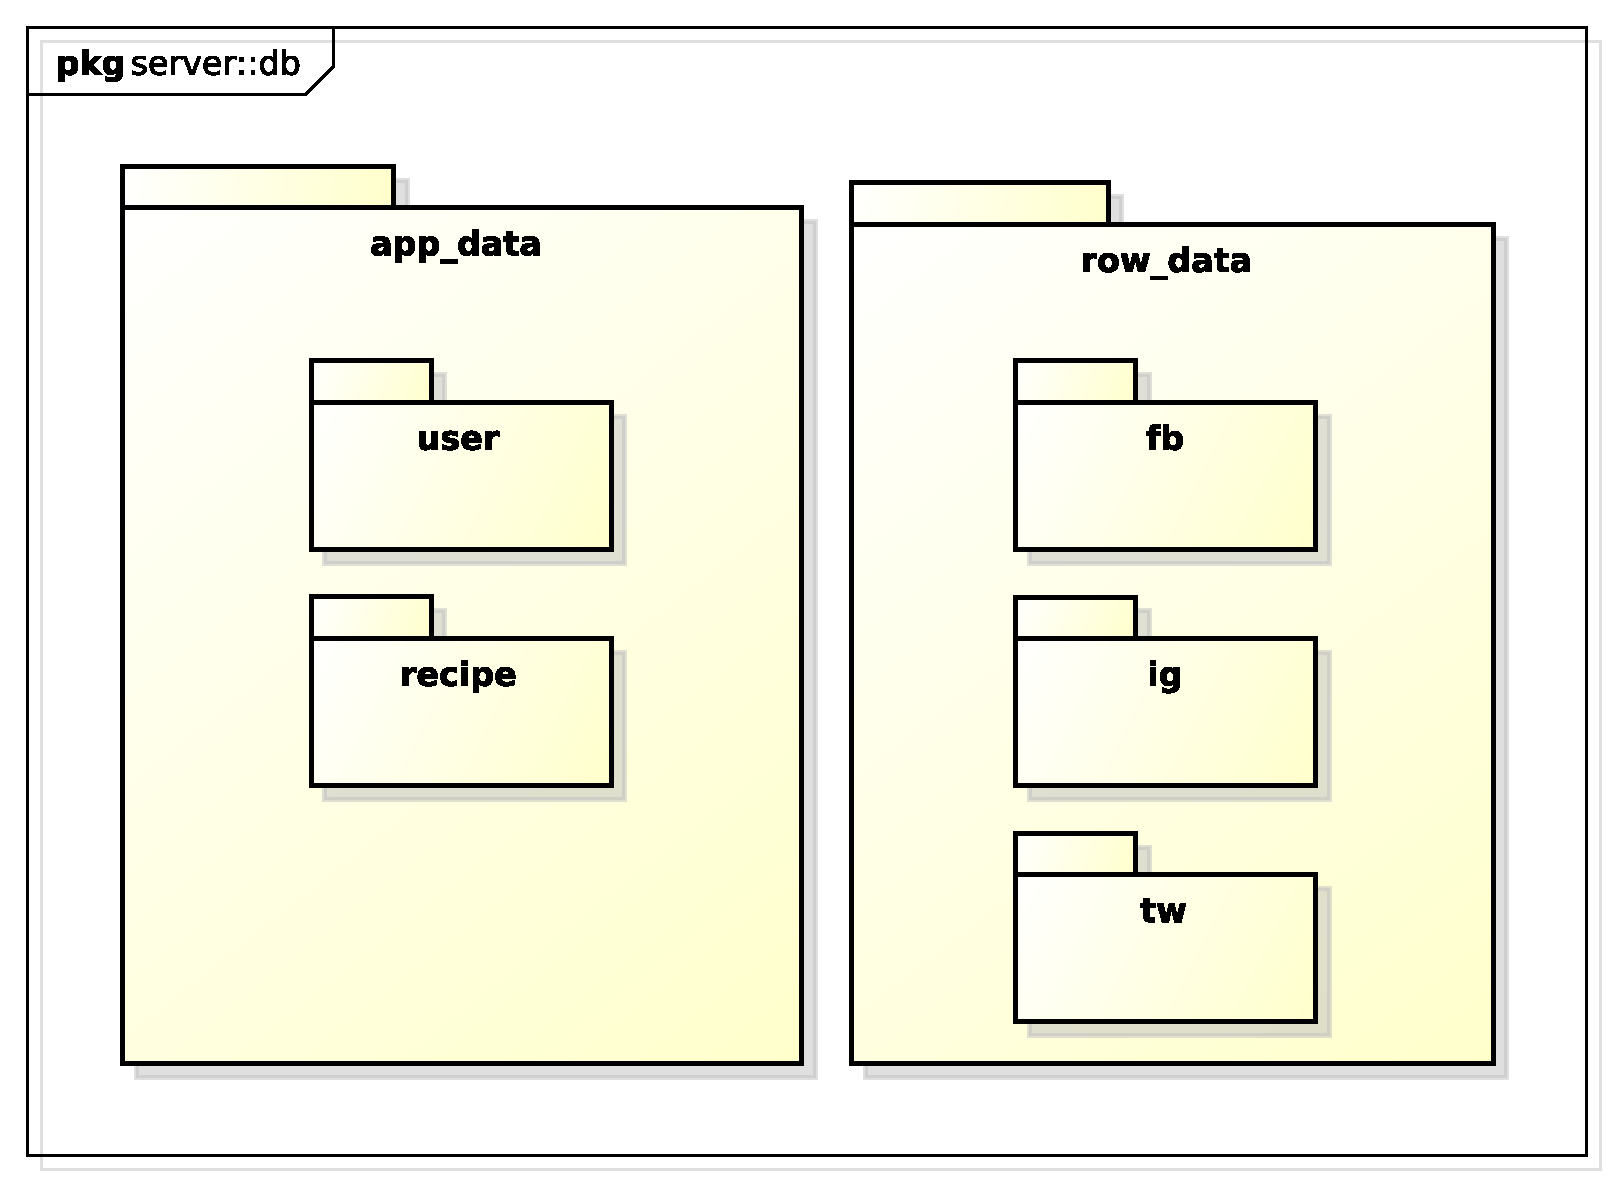
\includegraphics[scale=0.5]{./images/server/db.pdf}}
		\caption{Package - server::db}
	\end{figure}
	\begin{itemize}
		\item \textbf{Descrizione}: è il package che contiene le componenti che gestiscono e mantengono coerente la base di dati. Esse utilizzano standard proprietari Google per la loro implementazione. Sono suddivise in due package: uno atto a rappresentare il modello dei dati grezzi, l'altro per parametri del software e degli utenti;
		\item \textbf{Padre}: server;
		\item \textbf{Package contenuti}:
			\begin{itemize}
				\item server::app\_data.
				\item server::raw\_data;
			\end{itemize}
	\end{itemize}

% subsubsection RAW_DATA
\subsubsection{server::db::raw\_data} % (fold)
\label{ssub:bdsm_app_server_raw_data}
	\begin{figure}[htbp]
		\centering
		\centerline{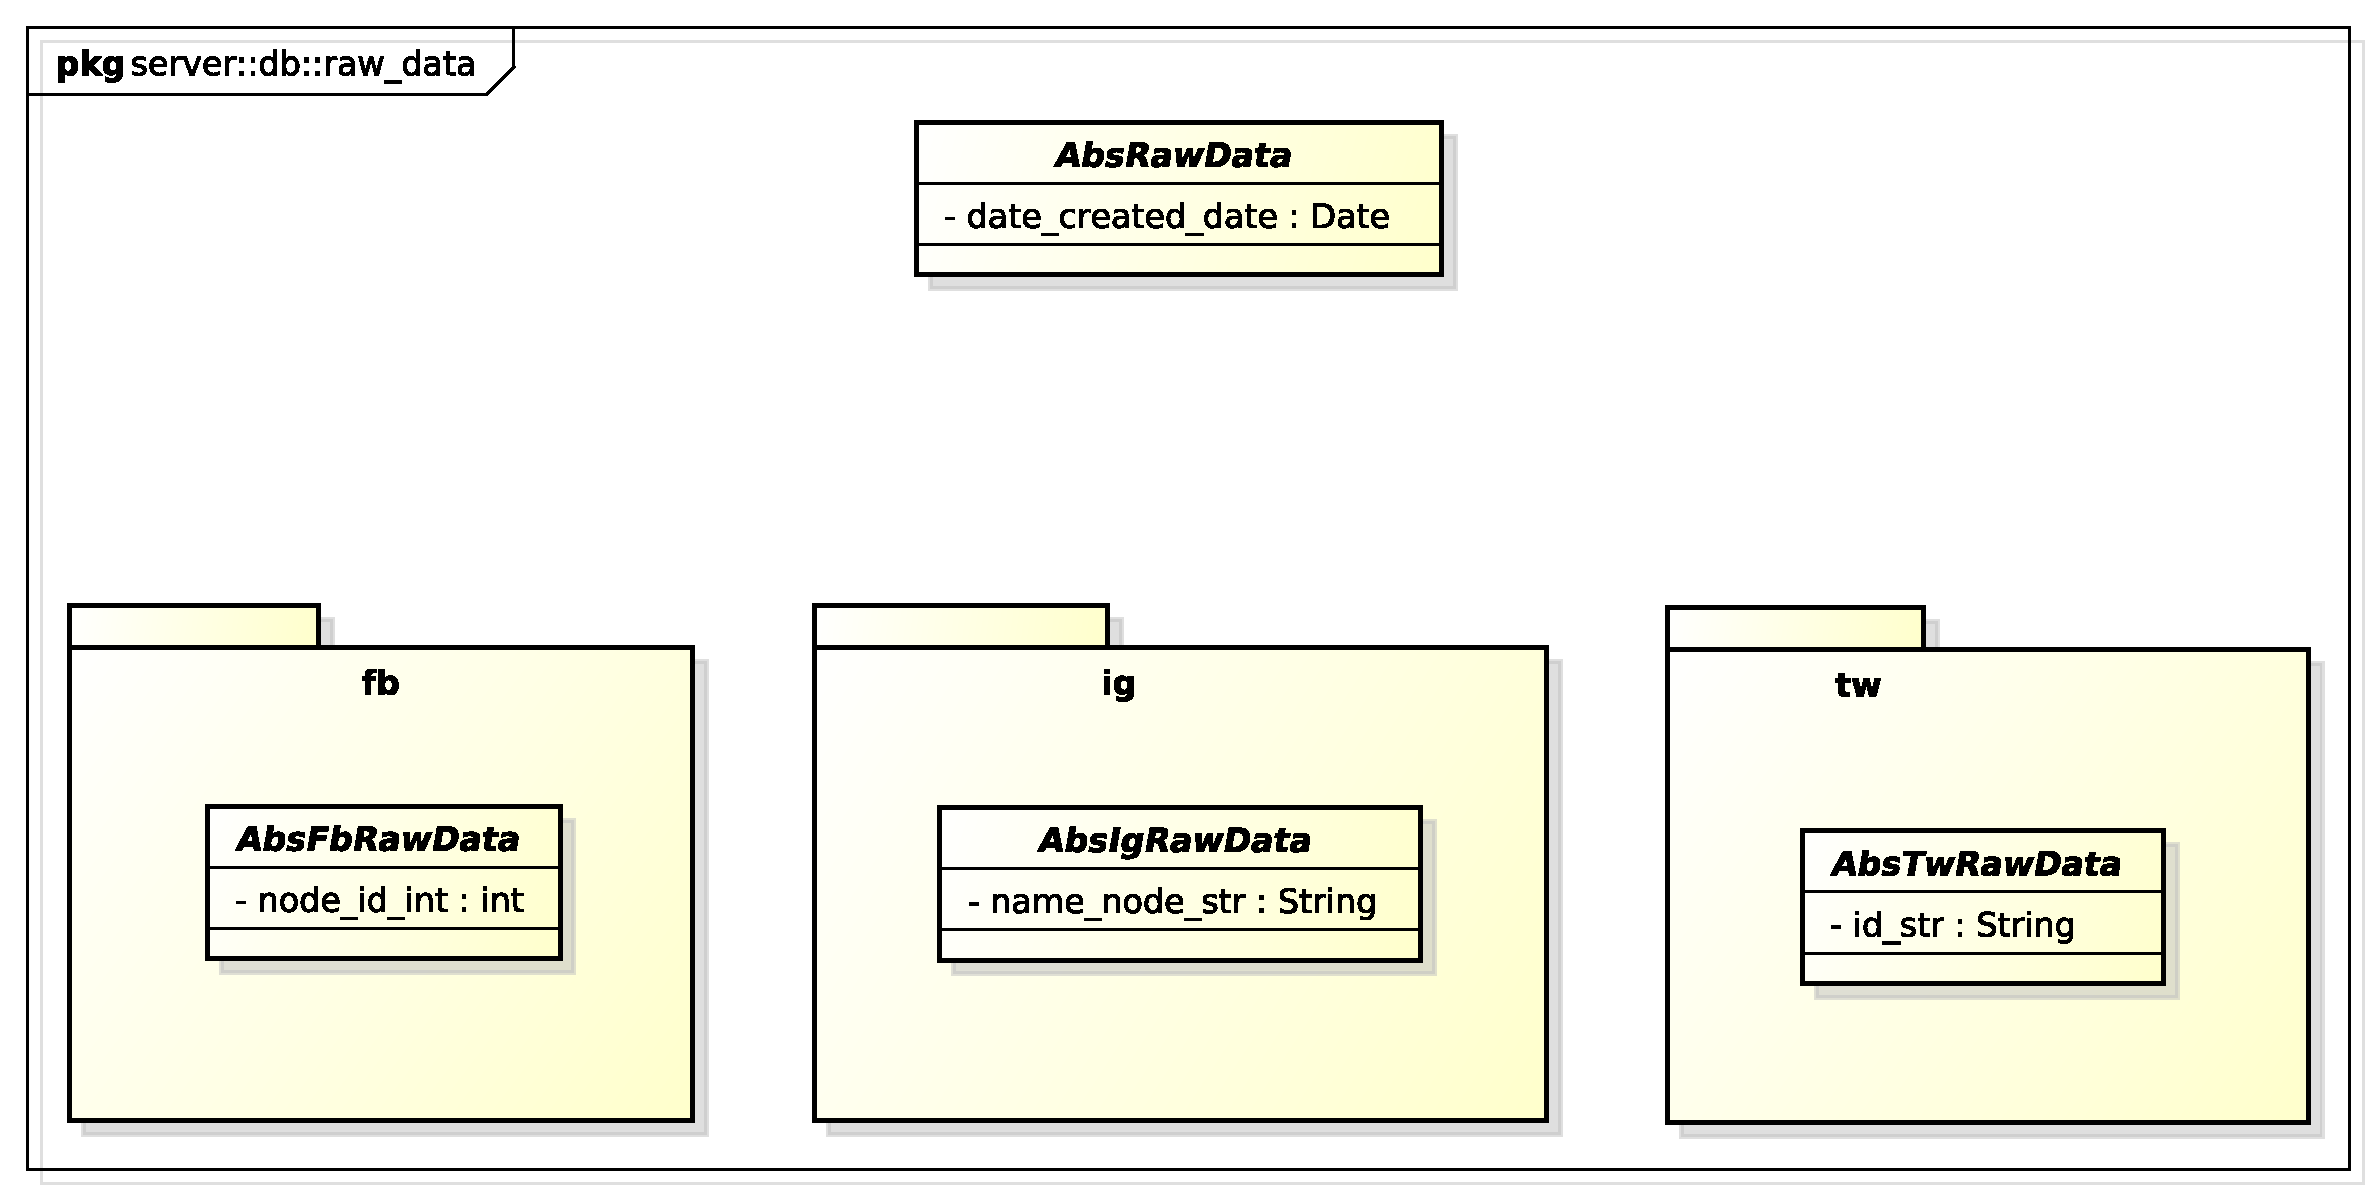
\includegraphics[scale=0.4]{./images/server/raw_data.pdf}}
		\caption{Package - server::db::raw\_data}
	\end{figure}
	\begin{itemize}
	\item \textbf{Descrizione}: package che definisce il modello dei dati grezzi ricavati dai vari social network;
		\item \textbf{Padre}: server::db;
		\item \textbf{Package contenuti}:
			\begin{itemize}
				\item server::db::raw\_data::fb
				\item server::db::raw\_data::tw
				\item server::db::raw\_data::ig
		\end{itemize}
	\end{itemize}

	\paragraph{Classi} % (fold)
		\subparagraph{server::db::raw\_data::AbsRawData} % (fold)
		\label{subp:bdsm_app_server_raw_data_absrawdata}
			\begin{itemize}
				\item \textbf{Descrizione}: classe astratta che definisce il modello di un dato grezzo;
				\item \textbf{Utilizzo}: la classe funge da padre per tutte le classi rappresentanti un dato grezzo;
				\item \textbf{Relazioni con altre classi}:
					\begin{itemize}
						\item server::db::raw\_data::fb::AbsFbRawData
						\item server::db::raw\_data::tw::AbsTwRawData
						\item server::db::raw\_data::ig::AbsIgRawData
						\item server::db::raw\_data::fb::RawFbPageTrend
						\item server::db::raw\_data::fb::RawFbEventTrend
						\item server::db::raw\_data::fb::RawFbPostTrendTrend
						\item server::db::raw\_data::tw::RawTwUserTrend
						\item server::db::raw\_data::tw::RawTwUserTweet
						\item server::db::raw\_data::ig::RawIgUserTrend
						\item server::db::raw\_data::ig::RawIgHashtagTrend
						\item server::db::raw\_data::ig::RawIgMedia
					\end{itemize}
				\item \textbf{Attributi}:
					\begin{itemize}
						\item \textcolor{forestgreen}{\texttt{+ date\_created\_date : Date}}
						\begin{description}
							\item \textbf{Descrizione}: data acquisizione dati grezzi
						\end{description}
					\end{itemize}
				\item \textbf{Metodi}: N/A
			\end{itemize}

		% subsubsection FACEBOOK
		\subsubsection{server::db::raw\_data::fb} % (fold)
		\label{ssub:bdsm_app_server_db_raw_data_fb}
		\begin{figure}[htbp]
			\centering
			\centerline{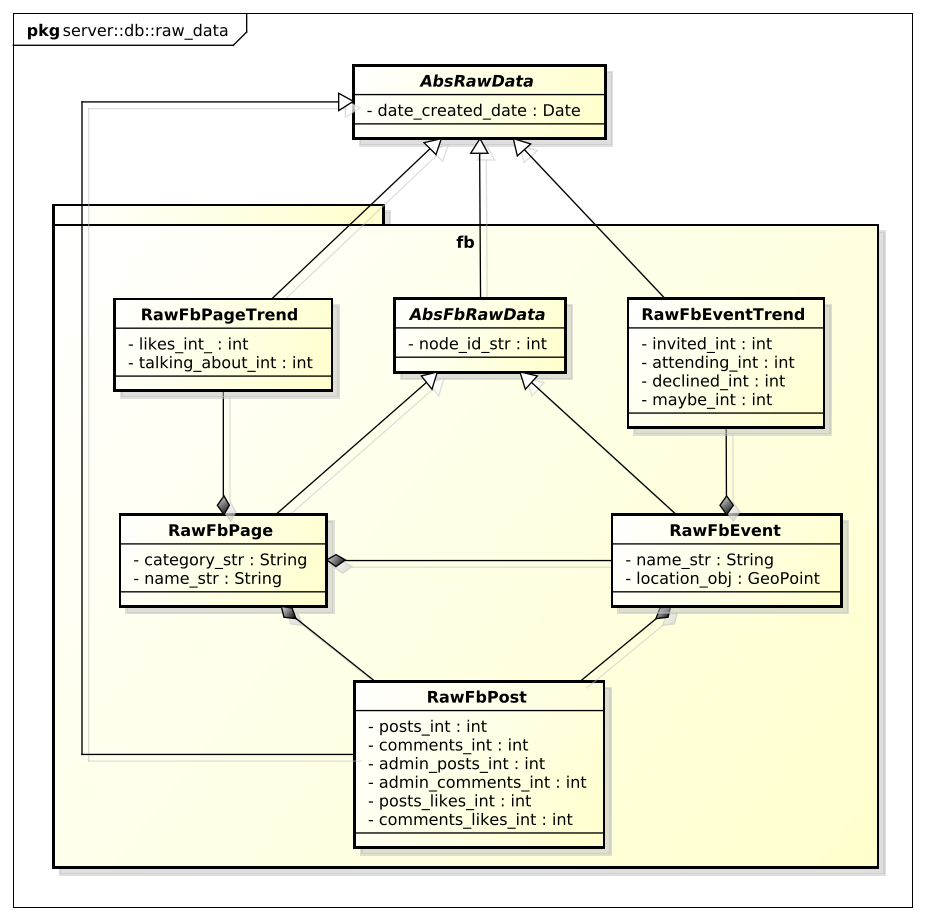
\includegraphics[scale=0.5]{./images/server/raw_data_fb.pdf}}
			\caption{Package - server::db::raw\_data::fb}
		\end{figure}
		\begin{itemize}
		  \item \textbf{Descrizione}:  è il package contenente le classi che definiscono i modelli dei dati grezzi relativi a Facebook;
		  \item \textbf{Padre}: server::db::raw\_data
		  \item \textbf{Interazione con altri componenti}:
		  	\begin{itemize}
		  		\item server::db
			\end{itemize}
		\end{itemize}
		% subsubsection

		\paragraph{Classi} % (fold)
			\subparagraph{server::db::raw\_data::fb::AbsFbRawData} % (fold)
			\label{subp:server_db_raw_data_fb_absfbrawdata}
				\begin{figure}[htbp]
					\centering
					\centerline{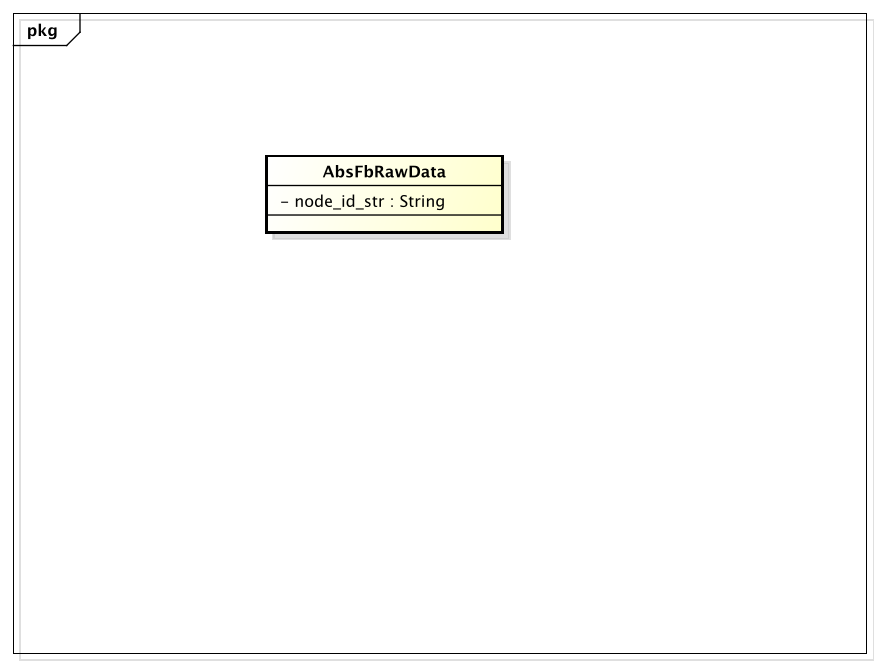
\includegraphics[scale=0.75]{./images/server/classes/db/abs_fb_raw_data.pdf}}
					\caption{Classe - server::db::raw\_data::fb::AbsFbRawData}
				\end{figure}
				\begin{itemize}
					\item \textbf{Descrizione}: classe astratta che definisce il modello dati grezzi relativi a Facebook;
					\item \textbf{Utilizzo}: la classe contiene l'id fornito dall'utente il quale permette di identificare univocamente la risorsa nel social media;
					\item \textbf{Classi ereditate}: server::db::raw\_data::AbsRawData
					\item \textbf{Attributi}:
					\begin{itemize}
						\item \textcolor{forestgreen}{\texttt{+ node\_id\_str : String}}
						\begin{description}
							\item \textbf{Descrizione}: codice identificativo di un evento o di una pagina Facebook.
						\end{description}
					\end{itemize}
					\item \textbf{Metodi}: N/A
				\end{itemize}
			% subparagraph server_db_raw_data_fb_absfbrawdata [end]


			\subparagraph{server::db::raw\_data::fb::RawFbPage} % (fold)
			\label{subp:server_db_raw_data_fb_rawfbpage}
				\begin{figure}[htbp]
					\centering
					\centerline{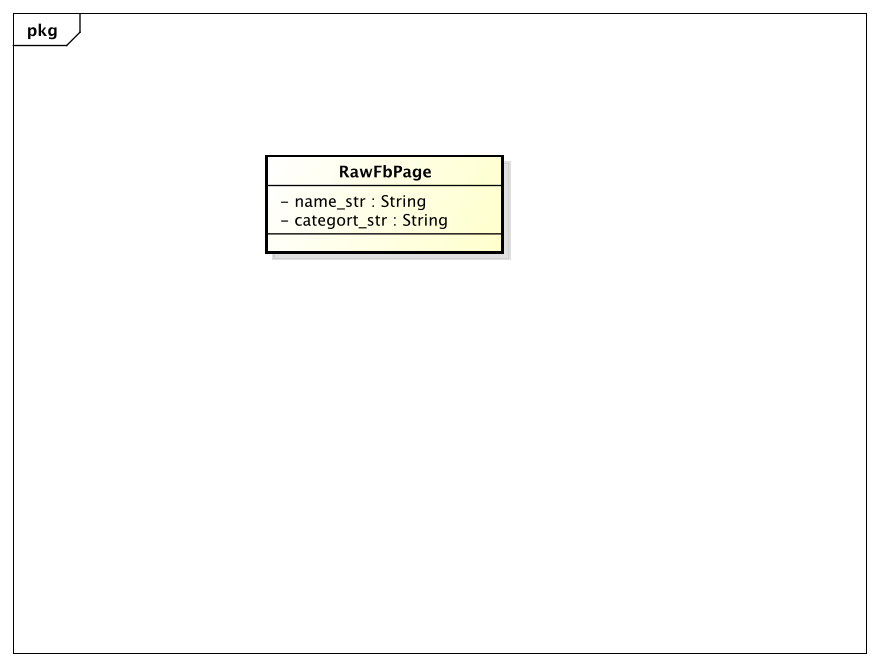
\includegraphics[scale=0.75]{./images/server/classes/db/raw_fb_page.pdf}}
					\caption{Classe - server::db::raw\_data::fb::RawFbPage}
				\end{figure}
				\begin{itemize}
					\item \textbf{Descrizione}: classe che rappresenta il modello di una pagina Facebook;
					\item \textbf{Utilizzo}: la classe fornisce metodi per memorizzare i dati statici di una pagina Facebook;
					\item \textbf{Classi ereditate}: server::db::raw\_data::AbsFbRawData
					\item \textbf{Relazioni con altre classi}:
						\begin{itemize}
							\item server::db::raw\_data::fb::RawFbEvent
							\item server::db::raw\_data::fb::RawFbPageTrend
							\item server::db::raw\_data::fb::RawFbPostTrend
						\end{itemize}
					\item \textbf{Attributi}:
					\begin{itemize}
						\item \textcolor{forestgreen}{\texttt{+ name\_str : String}}
						\begin{description}
							\item \textbf{Descrizione}: nome della pagina Facebook.
						\end{description}
						\item \textcolor{forestgreen}{\texttt{+ category\_str : String}}
						\begin{description}
							\item \textbf{Descrizione}: categoria della pagina Facebook.
						\end{description}
					\end{itemize}
					\item \textbf{Metodi}: N/A
				\end{itemize}
			% subparagraph server_db_raw_data_fb_rawfbpage [end]

			\subparagraph{server::db::raw\_data::fb::RawFbPageTrend} % (fold)
			\label{subp:server_db_raw_data_fb_rowfbpagetrend}
				\begin{figure}[htbp]
					\centering
					\centerline{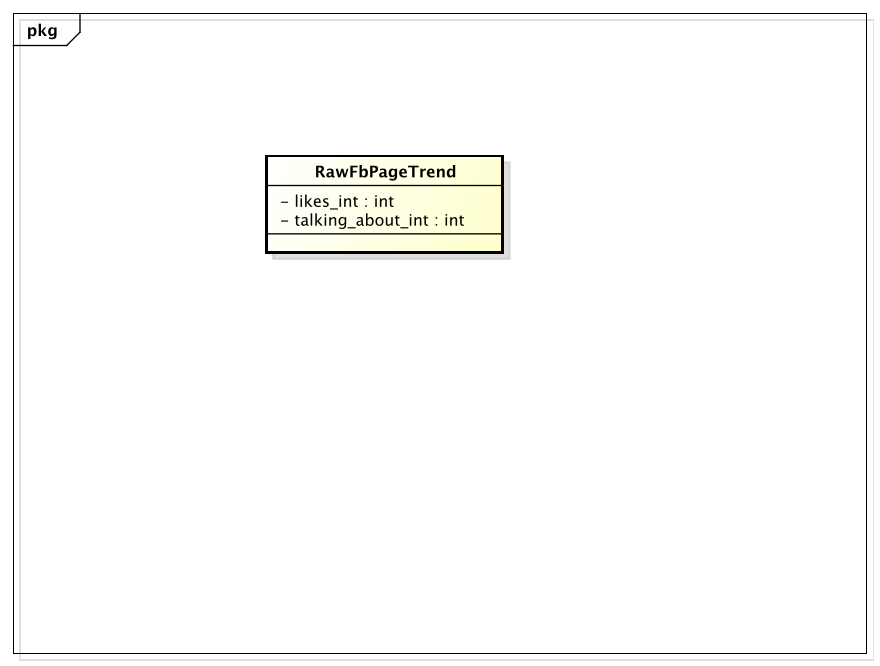
\includegraphics[scale=0.75]{./images/server/classes/db/raw_fb_page_trend.pdf}}
					\caption{Classe - server::db::raw\_data::fb::RawFbPageTrend}
				\end{figure}
				\begin{itemize}
					\item \textbf{Descrizione}: classe che rappresenta il modello del trend dei dati una pagina Facebook;
					\item \textbf{Utilizzo}: la classe viene utilizzata per memorizzare e il numero di like e di talking about di ogni singola pagina. Come per tutti gli oggetti di tipo trend, vengono ricavati i dati fino a 3 giorni prima della creazione dell'oggetto;
					\item \textbf{Classi ereditate}: server::db::raw\_data::AbsRawData
					\item \textbf{Attributi}:
					\begin{itemize}
						\item \textcolor{forestgreen}{\texttt{+ likes\_int : int}}
						\begin{description}
							\item \textbf{Descrizione}: numero dei likes di una determinata pagina Facebook,
						\end{description}
						\item \textcolor{forestgreen}{\texttt{+ talking\_about\_int : int}}
						\begin{description}
							\item \textbf{Descrizione}: numero di talking about di una determinata pagina Facebook.
						\end{description}
					\end{itemize}
					\item \textbf{Metodi}: N/A
				\end{itemize}
			% subparagraph server_db_raw_data_fb_rowfbpagetrend [end]


			\subparagraph{server::db::raw\_data::fb::RawFbEvent} % (fold)
			\label{subp:server_db_raw_data_fb_rawfbevent}
				\begin{figure}[htbp]
					\centering
					\centerline{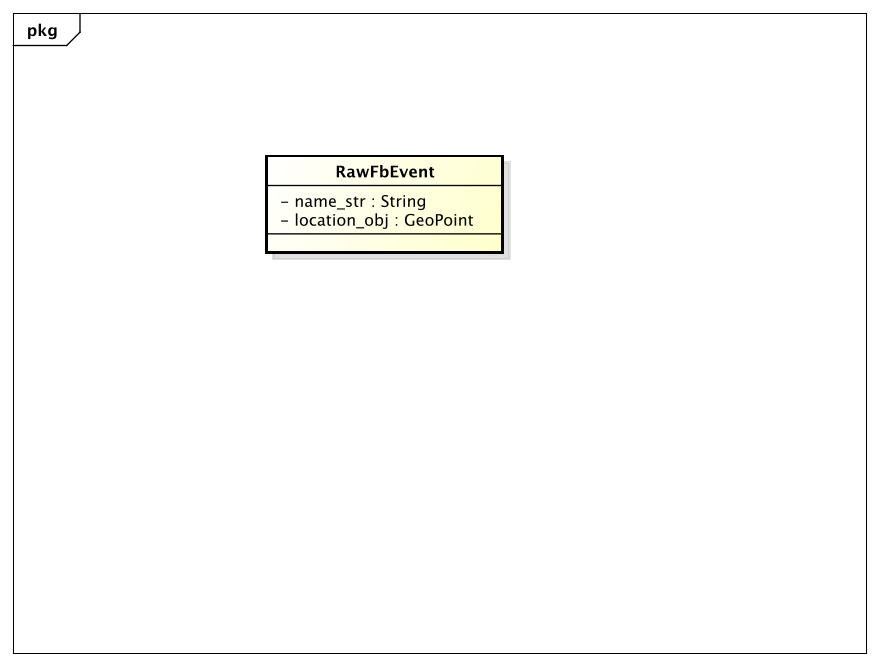
\includegraphics[scale=0.75]{./images/server/classes/db/raw_fb_event.pdf}}
					\caption{Classe - server::db::raw\_data::fb::RawFbEvent}
				\end{figure}
				\begin{itemize}
					\item \textbf{Descrizione}: classe che rappresenta il modello di un evento Facebook;
					\item \textbf{Utilizzo}: la classe fornisce metodi per memorizzare i dati statici di un evento Facebook;
					\item \textbf{Classi ereditate}: server::db::raw\_data::AbsFbRawData
					\item \textbf{Relazioni con altre classi}:
						\begin{itemize}
							\item server::db::raw\_data::fb::RawFbEventTrend
							\item server::db::raw\_data::fb::RawFbPostTrend
						\end{itemize}
					\item \textbf{Attributi}:
					\begin{itemize}
						\item \textcolor{forestgreen}{\texttt{+ name\_str : String}}
						\begin{description}
							\item \textbf{Descrizione}: nome dell'evento Facebook.
						\end{description}
						\item \textcolor{forestgreen}{\texttt{+ location\_obj : GeoPoint}}
						\begin{description}
							\item \textbf{Descrizione}: location dell'evento espressa in latitudine e longitudine.
						\end{description}
					\end{itemize}
					\item \textbf{Metodi}: N/A
				\end{itemize}
			% subparagraph server_db_raw_data_fb_rawfbevent [end]

			\subparagraph{server::db::raw\_data::fb::RawFbEventTrend} % (fold)
			\label{subp:server_db_raw_data_fb_rowfbeventtrend}
				\begin{figure}[htbp]
					\centering
					\centerline{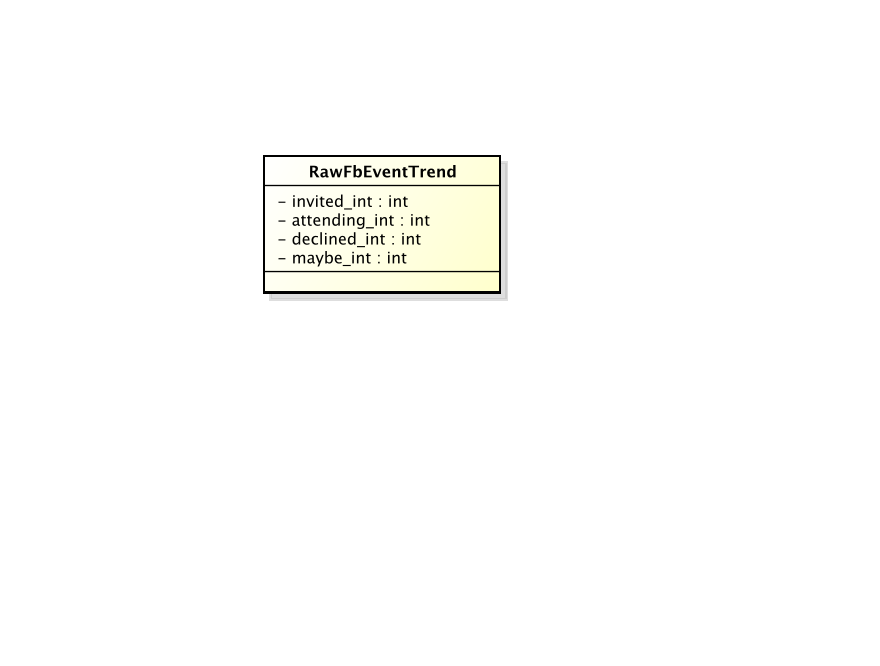
\includegraphics[scale=0.75]{./images/server/classes/db/raw_fb_event_trend.pdf}}
					\caption{Classe - server::db::raw\_data::fb::RawFbEventTrend}
				\end{figure}
				\begin{itemize}
					\item \textbf{Descrizione}: classe che rappresenta il modello del trend di un evento su Facebook;
					\item \textbf{Utilizzo}: la classe viene utilizzata per memorizzare il numero di utenti invitati, partecipanti e non di un evento. Come per tutti gli oggetti di tipo trend, vengono ricavati i dati fino a 3 giorni prima della creazione dell'oggetto;
					\item \textbf{Classi ereditate}: server::db::raw\_data::AbsRawData
					\item \textbf{Attributi}:
					\begin{itemize}
						\item \textcolor{forestgreen}{\texttt{+ invited\_int : int}}
						\begin{description}
							\item \textbf{Descrizione}: numero delle persone invitate all'evento Facebook.
						\end{description}
						\item \textcolor{forestgreen}{\texttt{+ attending\_int : int}}
						\begin{description}
							\item \textbf{Descrizione}: numero persone partecipanti all'evento Facebook
						\end{description}
						\item \textcolor{forestgreen}{\texttt{+ declined\_int : int}}
						\begin{description}
							\item \textbf{Descrizione}: numero persone che hanno rifiutato la partecipazione all'evento Facebook.
						\end{description}
						\item \textcolor{forestgreen}{\texttt{+ maybe\_int : int}}
						\begin{description}
							\item \textbf{Descrizione}: numero persone incerte se partecipare all'evento Facebook.
						\end{description}
					\end{itemize}
					\item \textbf{Metodi}: N/A
				\end{itemize}
			% subparagraph server_db_raw_data_fb_rowfbeventtrend [end]


			\subparagraph{server::db::raw\_data::fb::RawFbPostTrend} % (fold)
			\label{subp:server_db_raw_data_fb_RawFbPostTrend}
				\begin{figure}[htbp]
					\centering
					\centerline{\includegraphics[scale=0.75]{./images/server/classes/db/raw_fb_post_trend.pdf}}
					\caption{Classe - server::db::raw\_data::fb::RawFbPostTrend}
				\end{figure}
				\begin{itemize}
					\item \textbf{Descrizione}: classe che rappresenta il modello del trend dei post di una pagina o di un evento su Facebook;
					\item \textbf{Utilizzo}: viene utilizzata per memorizzare i dati relativi al trend dei post di una pagina o un pagina o evento Facebook. Come per tutti gli oggetti di tipo trend, vengono ricavati i dati fino a 3 giorni prima della creazione dell'oggetto;
					\item \textbf{Attributi}:
					\begin{itemize}
						\item \textcolor{forestgreen}{\texttt{+ posts\_int : int}}
						\begin{description}
							\item \textbf{Descrizione}: numero dei post presenti nella pagina o nell'evento.
						\end{description}
						\item \textcolor{forestgreen}{\texttt{+ comments\_int : int}}
						\begin{description}
							\item \textbf{Descrizione}: numero totale di commenti ai post della pagina o dell'evento.
						\end{description}
						\item \textcolor{forestgreen}{\texttt{+ admin\_posts\_int : int}}
						\begin{description}
							\item \textbf{Descrizione}: numero dei post effettuati esclusivamente da una pagina Facebook e non da terzi.
						\end{description}
						\item \textcolor{forestgreen}{\texttt{+ admin\_comments\_int : int}}
						\begin{description}
							\item \textbf{Descrizione}: numero dei commenti effettuati esclusivamente da una pagina Facebook e non da terzi.
						\end{description}
						\item \textcolor{forestgreen}{\texttt{+ posts\_like\_int : int}}
						\begin{description}
							\item \textbf{Descrizione}: numero totale dei likes ai post di una pagina o evento Facebook.
						\end{description}
						\item \textcolor{forestgreen}{\texttt{+ comments\_like\_int : int}}
						\begin{description}
							\item \textbf{Descrizione}: numero totale ai likes dei commenti presenti nei post di una pagina o evento Facebook.
						\end{description}
					\end{itemize}
					\item \textbf{Metodi}: N/A
				\end{itemize}
			% subparagraph server_db_raw_data_fb_RawFbPostTrend [end]


		% subsubsection TWITTER
		\subsubsection{server::db::raw\_data::tw} % (fold)
		\label{ssub:bdsm_app_server_db_raw_data_tw}
		\begin{figure}[htbp]
			\centering
			\centerline{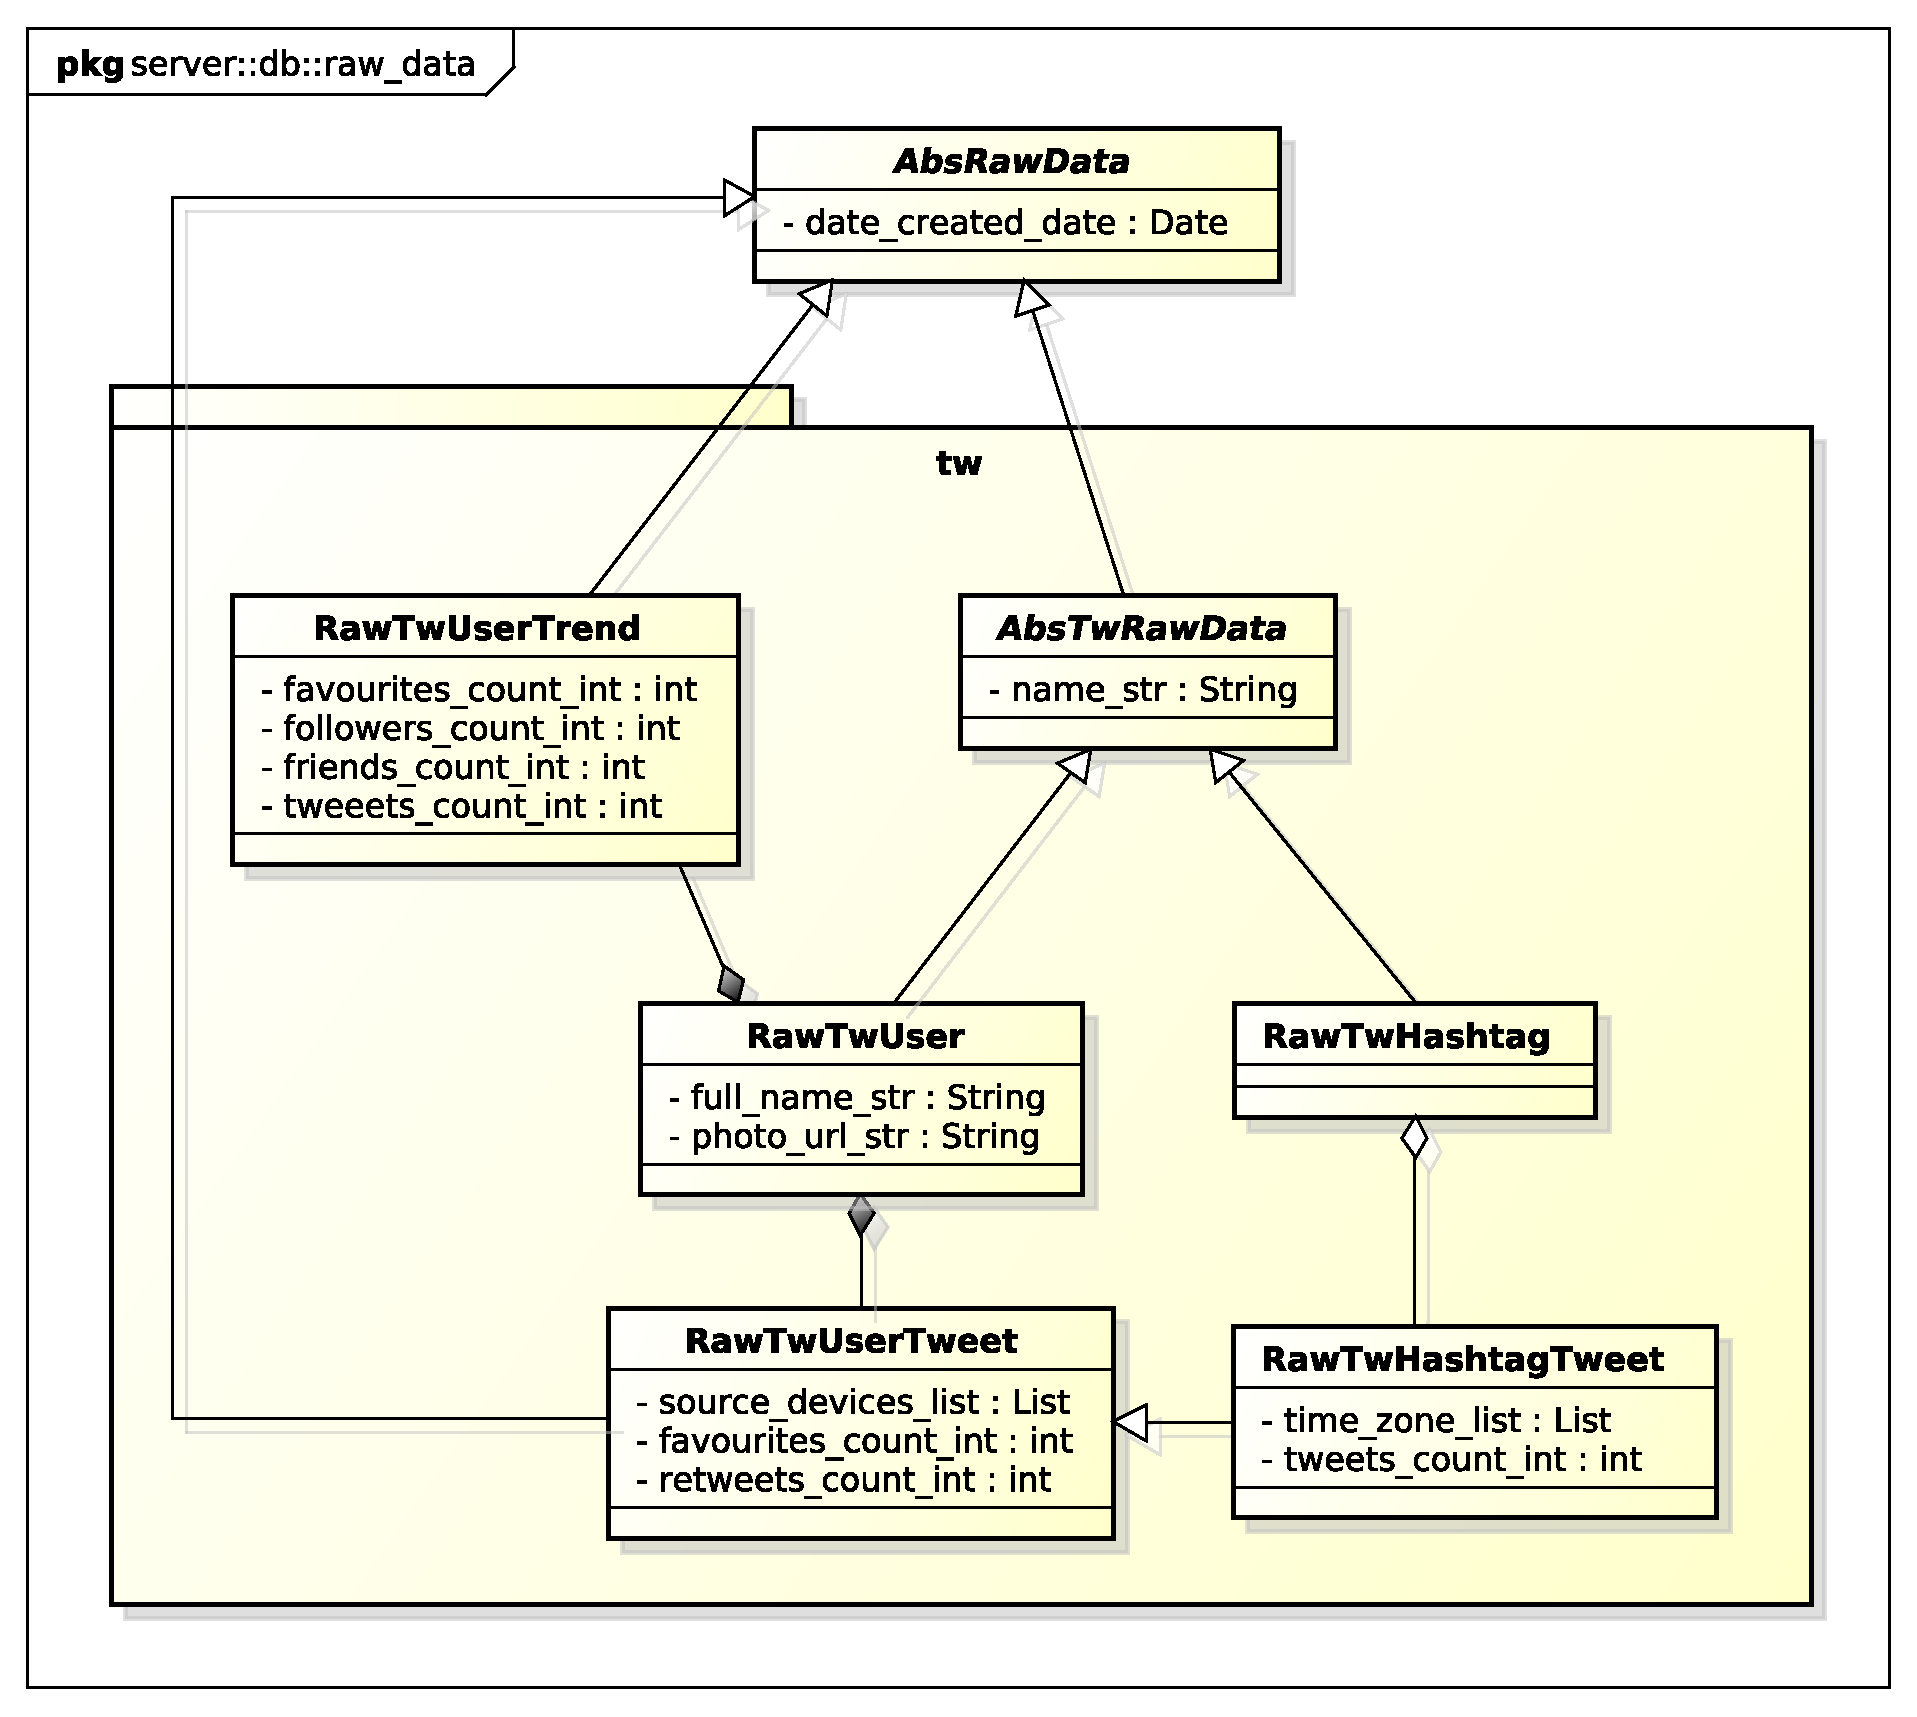
\includegraphics[scale=0.45]{./images/server/raw_data_tw.pdf}}
			\caption{Package - server::db::raw\_data::tw}
		\end{figure}

		\begin{itemize}
		  \item \textbf{Descrizione}: è il package contenente le classi che definiscono i modelli dei dati grezzi relativi a Twitter;
		  \item \textbf{Padre}: server::db::raw\_data
		  \item \textbf{Interazione con altri componenti}:
		  	\begin{itemize}
		  		\item server::db
			\end{itemize}
		\end{itemize}
		% subsubsection

		\paragraph{Classi} % (fold)


		\subparagraph{server::db::raw\_data::tw::AbsTwRawData} % (fold)
		\label{subp:server_db_raw_data_tw_abstwrawdata}
			\begin{figure}[htbp]
				\centering
				\centerline{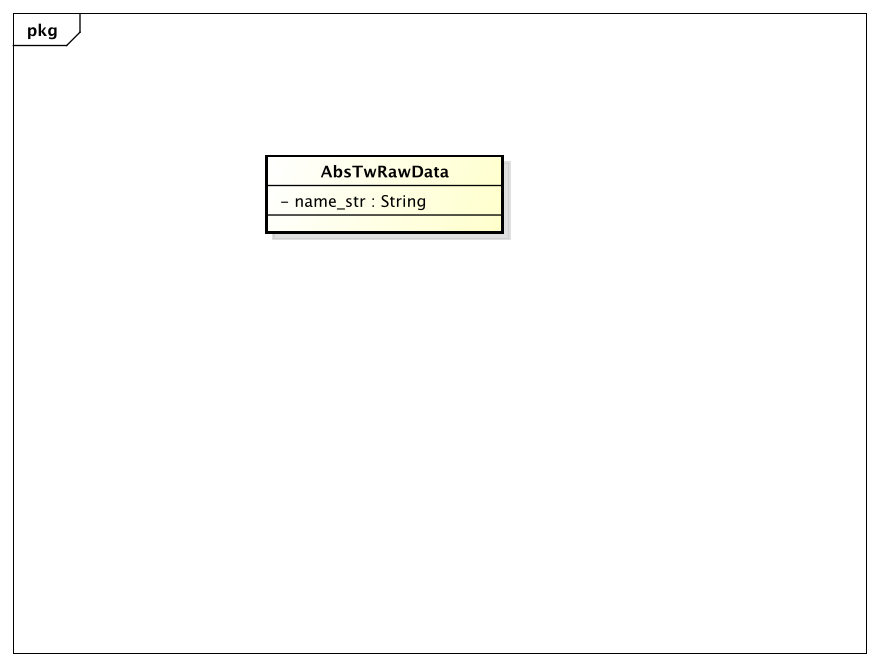
\includegraphics[scale=0.75]{./images/server/classes/db/abs_tw_raw_data.pdf}}
				\caption{Classe - server::db::raw\_data::tw::AbsTwRawData}
			\end{figure}
			\begin{itemize}
				\item \textbf{Descrizione}: classe astratta che definisce il modello dati grezzi relativi a Twitter;
				\item \textbf{Utilizzo}: la classe contiene l'id fornito dall'utente il quale permette di identificare univocamente la risorsa nel social media;
				\item \textbf{Classi ereditate}: server::db::raw\_data::AbsRawData
				\item \textbf{Attributi}:
					\begin{itemize}
						\item \textcolor{forestgreen}{\texttt{+ name\_str : String}}
						\begin{description}
							\item \textbf{Descrizione}: nome identificativo della pagina o dell'hashtag Twitter.
						\end{description}
					\end{itemize}
				\item \textbf{Metodi}: N/A
			\end{itemize}
		% subparagraph server_db_raw_data_tw_abstwrawdata [end]


		\subparagraph{server::db::raw\_data::tw::RawTwUser} % (fold)
		\label{subp:server_db_raw_data_tw_rawtwuser}
			\begin{figure}[htbp]
				\centering
				\centerline{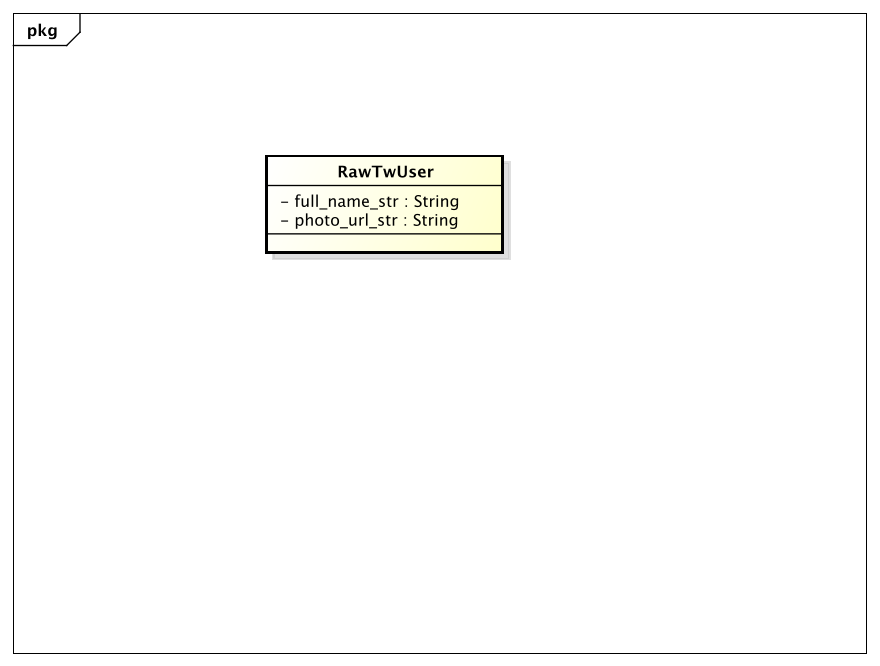
\includegraphics[scale=0.75]{./images/server/classes/db/raw_tw_user.pdf}}
				\caption{Classe - server::db::raw\_data::tw::RawTwUser}
			\end{figure}
			\begin{itemize}
				\item \textbf{Descrizione}: classe che definisce il modello dei dati di un utente Twitter;
				\item \textbf{Utilizzo}: la classe viene utilizzata per fornire una descrizione completa dell'utente Twitter. Vengono forniti metodi automatici per il conteggio dei parametri che verranno utilizzati per seguire un trend;;
				\item \textbf{Classi ereditate}: server::db::raw\_data::AbsTwRawData
				\item \textbf{Relazioni con altre classi}:
					\begin{itemize}
						\item server::db::raw\_data::tw::RawTwUserTrend
						\item server::db::raw\_data::tw::RawTwUserTweet
					\end{itemize}
				\item \textbf{Attributi}:
					\begin{itemize}
						\item \textcolor{forestgreen}{\texttt{+ full\_name\_str : String}}
						\begin{description}
							\item \textbf{Descrizione}: nome completo dell'utente Twitter.
						\end{description}
						\item \textcolor{forestgreen}{\texttt{+ photo\_url\_str : String}}
						\begin{description}
							\item \textbf{Descrizione}: indirizzo url della foto profilo dell'utente Twitter.
						\end{description}
					\end{itemize}
				\item \textbf{Metodi}: N/A
			\end{itemize}
		% subparagraph server_db_raw_data_tw_rawtwuser [end]


		\subparagraph{server::db::raw\_data::tw::RawTwUserTrend} % (fold)
		\label{subp:server_db_raw_data_tw_rawtwusertrend}
			\begin{figure}[htbp]
				\centering
				\centerline{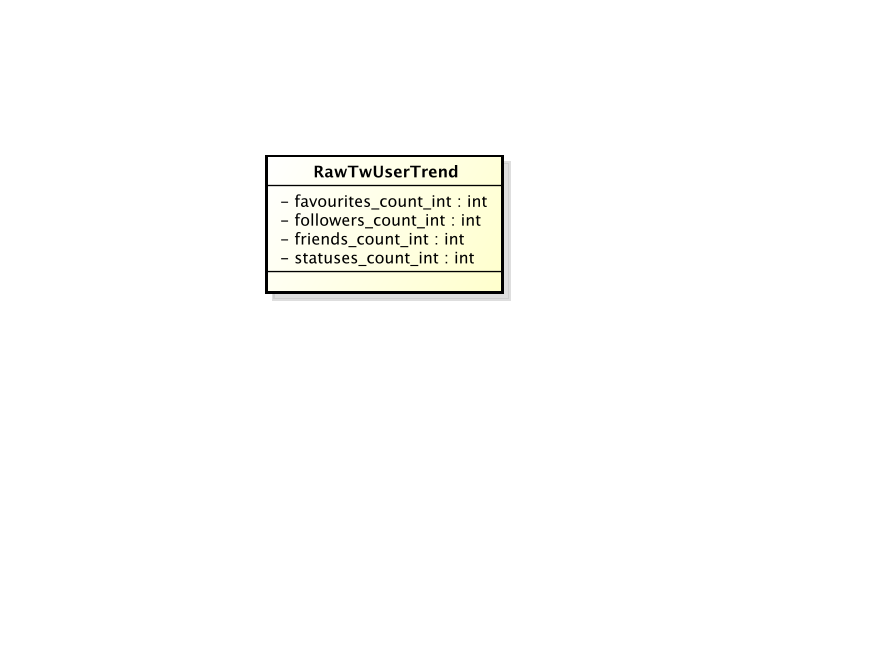
\includegraphics[scale=0.75]{./images/server/classes/db/raw_tw_user_trend.pdf}}
				\caption{Classe - server::db::raw\_data::tw::RawTwUserTrend}
			\end{figure}
			\begin{itemize}
				\item \textbf{Descrizione}: classe che definisce il modello dei dati del trend di un utente Twitter;
				\item \textbf{Utilizzo}: la classe viene utilizzata per memorizzare il numero di favoriti, di followers, di friends e statuses di un determinato utente Twitter. Come per tutti gli oggetti di tipo trend, vengono ricavati i dati fino a 3 giorni prima della creazione dell'oggetto;
				\item \textbf{Classi ereditate}: server::db::raw\_data::AbsTwRawData
				\item \textbf{Attributi}:
					\begin{itemize}
						\item \textcolor{forestgreen}{\texttt{+ favourites\_count\_int : int}}
						\begin{description}
							\item \textbf{Descrizione}: numero totale dei preferiti assegnati dall'utente.
						\end{description}
						\item \textcolor{forestgreen}{\texttt{+ followers\_count\_int : int}}
						\begin{description}
							\item \textbf{Descrizione}: numero dei followers di un utente Twitter.
						\end{description}
						\item \textcolor{forestgreen}{\texttt{+ friends\_count\_int : int}}
						\begin{description}
							\item \textbf{Descrizione}: numero dei following di un utente Twitter.
						\end{description}
						\item \textcolor{forestgreen}{\texttt{+ tweets\_count\_int : int}}
						\begin{description}
							\item \textbf{Descrizione}: numero di tweets di un utente Twitter.
						\end{description}
					\end{itemize}
				\item \textbf{Metodi}: N/A
			\end{itemize}
		% subparagraph server_db_raw_data_tw_rawigusertrend [end]


		\subparagraph{server::db::raw\_data::tw::RawTwUserTweet} % (fold)
		\label{subp:server_db_raw_data_tw_rawtwusertweet}
			\begin{figure}[htbp]
				\centering
				\centerline{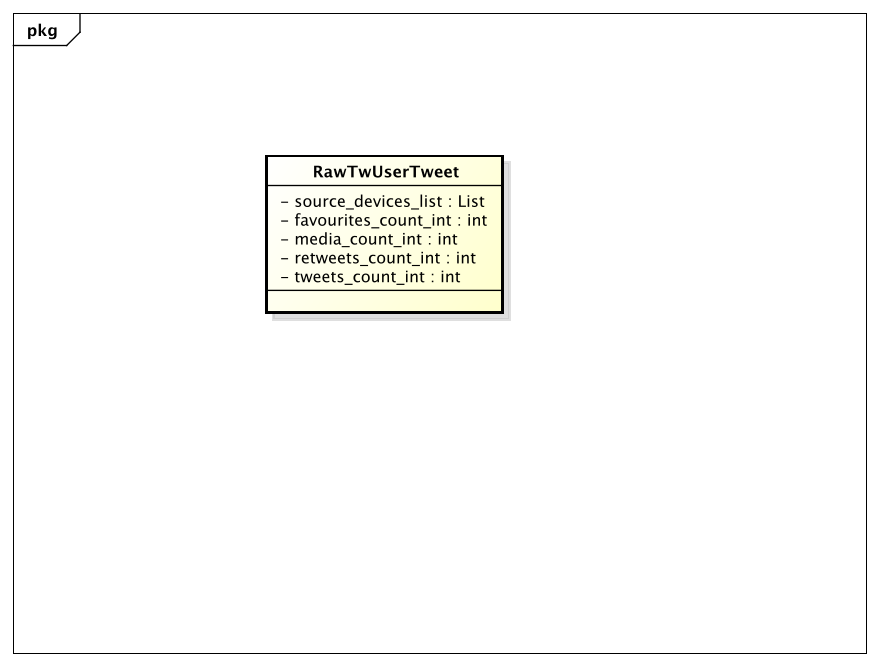
\includegraphics[scale=0.75]{./images/server/classes/db/raw_tw_user_tweet.pdf}}
				\caption{Classe - server::db::raw\_data::tw::RawTwUserTweet}
			\end{figure}
			\begin{itemize}
				\item \textbf{Descrizione}: classe che definisce il modello dei dati del trend dei tweet relativi ad un utente Twitter;
				\item \textbf{Utilizzo}: la classe viene utilizzata per fornire una descrizione dettagliata di un tweet creato da un utente specifico su Twitter;
				\item \textbf{Classi ereditate}: server::db::raw\_data::AbsRawData
				\item \textbf{Attributi}:
					\begin{itemize}
						\item \textcolor{forestgreen}{\texttt{+ source\_devices\_list : List}}
						\begin{description}
							\item \textbf{Descrizione}: lista composta da quantità e tipo dispositivi utilizzati in relazione ai tweet di un utente Twitter.
						\end{description}
						\item \textcolor{forestgreen}{\texttt{+ favourites\_count\_int : int}}
						\begin{description}
							\item \textbf{Descrizione}: totale dei preferiti aggiunti ai tweet di un utente.
						\end{description}
						\item \textcolor{forestgreen}{\texttt{+ retweets\_count\_int : int}}
						\begin{description}
							\item \textbf{Descrizione}: numero totale dei retweet ai tweets di utente Twitter.
						\end{description}
					\end{itemize}
				\item \textbf{Metodi}: N/A
			\end{itemize}
		% subparagraph server_db_raw_data_tw_rawtwusertweet [end]


		\subparagraph{server::db::raw\_data::tw::RawTwHashtag} % (fold)
		\label{subp:server_db_raw_data_tw_rawtwhashtag}
			\begin{itemize}
				\item \textbf{Descrizione}: classe che definisce il modello dei dati di un hashtag su Twitter;
				\item \textbf{Utilizzo}: la classe viene utilizzata per fornire una descrizione minimale di un hashtag su Twitter. Sebbene tale classe non presenti metodi o attributi, risulta molto utile per distinguere un hashtag Twitter da un'altra metrica effettuando un type checking;
				\item \textbf{Classi ereditate}: server::db::raw\_data::AbsTwRawData
				\item \textbf{Relazioni con altre classi}:
					\begin{itemize}
						\item server::db::raw\_data::tw::RawTwHashtagTweet
					\end{itemize}
				\item \textbf{Attributi}: N/A
				\item \textbf{Metodi}: N/A
			\end{itemize}
		% subparagraph server_db_raw_data_tw_rawtwhashtag [end]


		\subparagraph{server::db::raw\_data::tw::RawTwHashtagTweet} % (fold)
		\label{subp:server_db_raw_data_tw_rawtwhashtagtweet}
			\begin{figure}[htbp]
				\centering
				\centerline{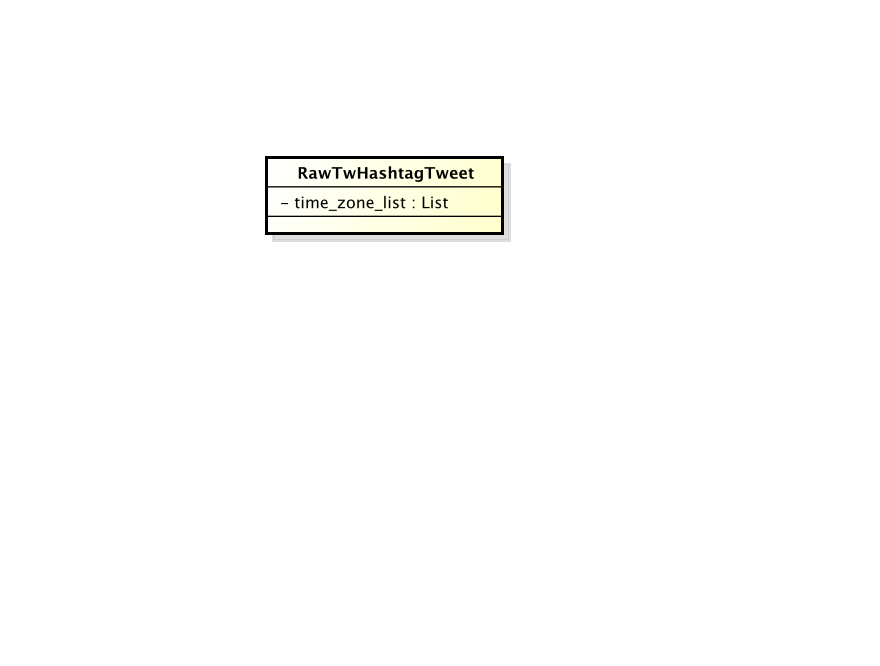
\includegraphics[scale=0.75]{./images/server/classes/db/raw_tw_hashtag_tweet.pdf}}
				\caption{Classe - server::db::raw\_data::tw::RawTwHashtagTweet}
			\end{figure}
			\begin{itemize}
				\item \textbf{Descrizione}: classe che definisce il modello dei dati del trend dei tweet relativi ad un hashtag Twitter;
				\item \textbf{Utilizzo}: la classe viene utilizzata per fornire una descrizione della locazione spaziale di un tweet relativo all'hashtag su Twitter. Come per tutti gli oggetti di tipo trend, vengono ricavati i dati fino a 3 giorni prima della creazione dell'oggetto;
				\item \textbf{Classi ereditate}: server::db::raw\_data::RawTwUserTweet
				\item \textbf{Attributi}:
					\begin{itemize}
						\item \textcolor{forestgreen}{\texttt{+ time\_zone\_list : List}}
						\begin{description}
							\item \textbf{Descrizione}: contiene informazioni sulle timezone ricavate dai vari tweet contenenti un determinato hashtag Twitter e dalle occorrenze delle stesse.
						\end{description}
						\item \textcolor{forestgreen}{\texttt{+ tweets\_count\_int : int}}
						\begin{description}
							\item \textbf{Descrizione}: totale dei tweet contenenti un determinato hashtag.
						\end{description}
					\end{itemize}
				\item \textbf{Metodi}: N/A
			\end{itemize}
		% subparagraph server_db_raw_data_tw_rawtwhashtagtweet [end]


		% subsubsection INSTAGRAM
		\subsubsection{server::db::raw\_data::ig} % (fold)
		\label{ssub:bdsm_app_server_db_raw_data_ig}
		\begin{figure}[htbp]
			\centering
			\centerline{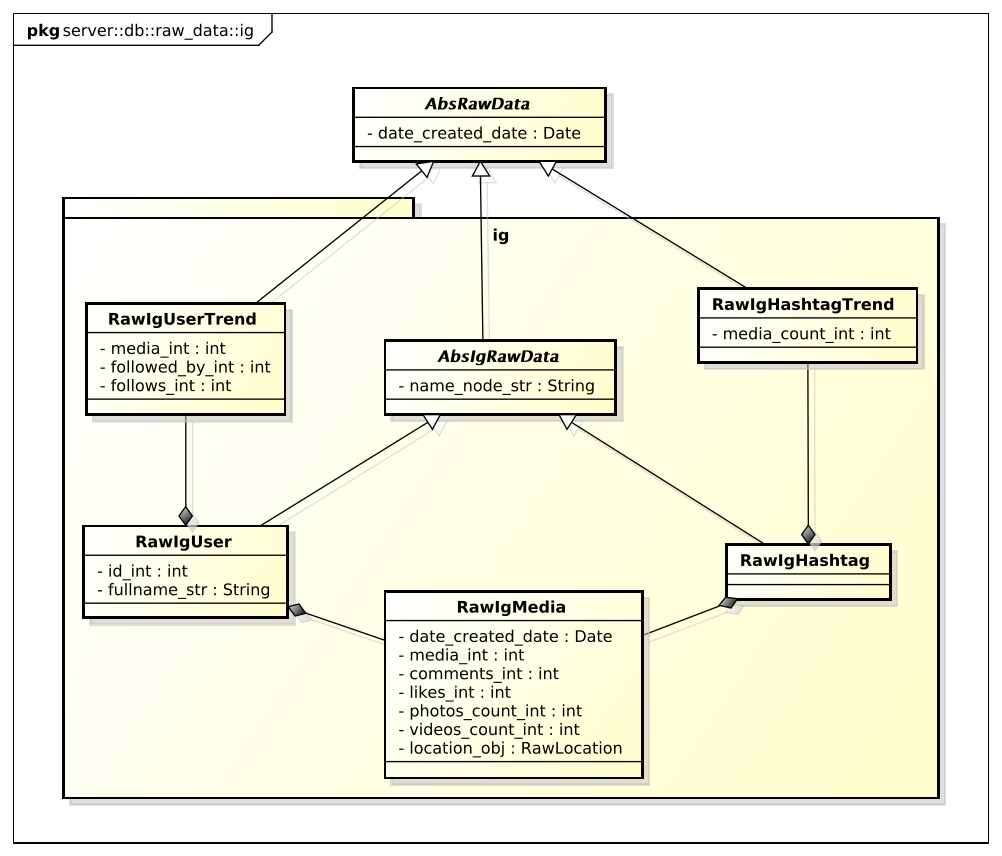
\includegraphics[scale=0.5]{./images/server/raw_data_ig.pdf}}
			\caption{Package - server::db::raw\_data::ig}
		\end{figure}

		\begin{itemize}
		  \item \textbf{Descrizione}: è il package contenente le classi che definiscono i modelli dei dati grezzi relativi a Instagram;
		  \item \textbf{Padre}: server::db::raw\_data
		  \item \textbf{Interazione con altri componenti}:
		  	\begin{itemize}
		  		\item server::db
				\end{itemize}
		\end{itemize}
		% subsubsection

		\paragraph{Classi} % (fold)


		\subparagraph{server::db::raw\_data::ig::AbsIgRawData} % (fold)
		\label{subp:server_db_raw_data_ig_absigrawdata}
			\begin{figure}[htbp]
				\centering
				\centerline{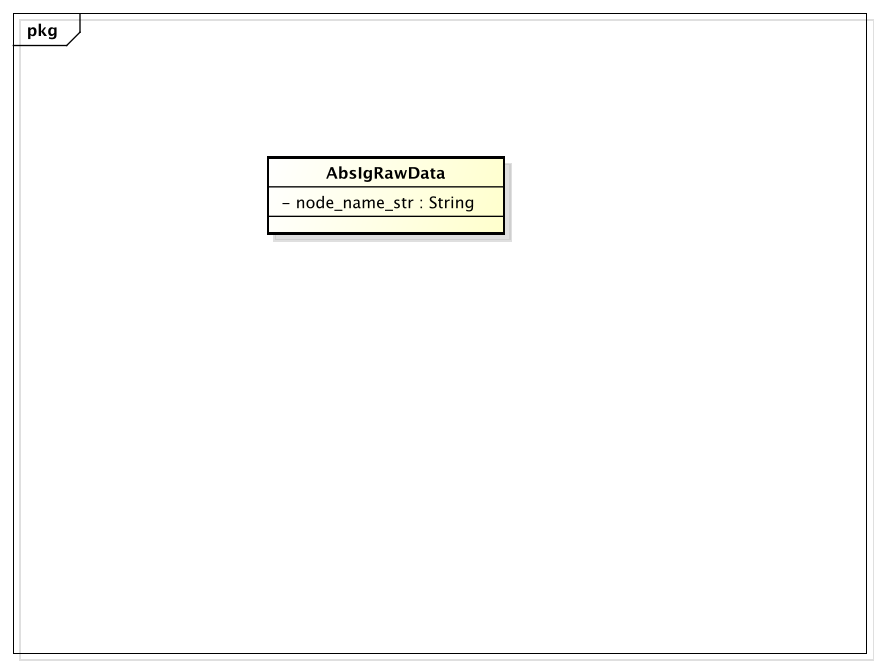
\includegraphics[scale=0.75]{./images/server/classes/db/abs_ig_raw_data.pdf}}
				\caption{Classe - server::db::raw\_data::ig::AbsIgRawData}
			\end{figure}
			\begin{itemize}
				\item \textbf{Descrizione}: classe astratta che definisce il modello dei dati grezzi relativi ad Instagram;
				\item \textbf{Utilizzo}: la classe contiene l'id fornito dall'utente il quale permette di identificare univocamente la risorsa nel social media;
				\item \textbf{Classi ereditate}: server::db::raw\_data::AbsRawData
				\item \textbf{Attributi}:
					\begin{itemize}
						\item \textcolor{forestgreen}{\texttt{+ node\_name\_str : String}}
						\begin{description}
							\item \textbf{Descrizione}: nome identificativo di un utente o di un hashtag Instagram.
						\end{description}
					\end{itemize}
				\item \textbf{Metodi}: N/A
			\end{itemize}
		% subparagraph server_db_raw_data_ig_absigrawdata [end]


		\subparagraph{server::db::raw\_data::ig::RawIgUser} % (fold)
		\label{subp:server_db_raw_data_ig_rawiguser}
			\begin{figure}[htbp]
				\centering
				\centerline{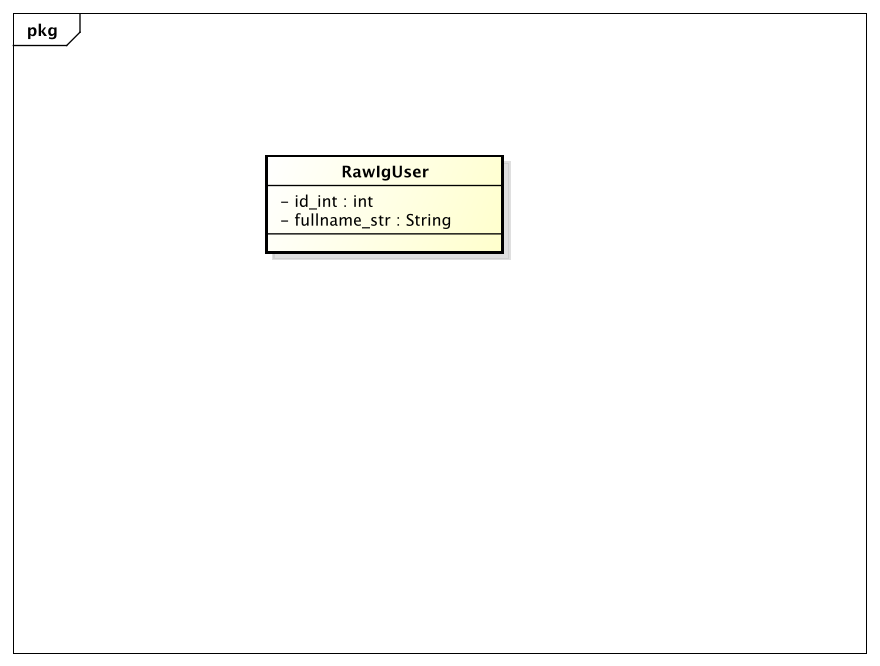
\includegraphics[scale=0.75]{./images/server/classes/db/raw_ig_user.pdf}}
				\caption{Classe - server::db::raw\_data::ig::RawIgUser}
			\end{figure}
			\begin{itemize}
				\item \textbf{Descrizione}: classe che definisce il modello dei dati di un utente Instagram;
				\item \textbf{Utilizzo}:  la classe viene utilizzata per memorizzare i dettagli di un utente Instagram;
				\item \textbf{Classi ereditate}: server::db::raw\_data::AbsIgRawData
				\item \textbf{Relazioni con altre classi}:
					\begin{itemize}
						\item server::db::raw\_data::ig::RawIgUserTrend
						\item server::db::raw\_data::ig::RawIgMedia
					\end{itemize}
				\item \textbf{Attributi}:
					\begin{itemize}
						\item \textcolor{forestgreen}{\texttt{+ id\_int : int}}
						\begin{description}
							\item \textbf{Descrizione}: numero identificativo di utente Instagram.
						\end{description}
						\item \textcolor{forestgreen}{\texttt{+ fullname\_str : String}}
						\begin{description}
							\item \textbf{Descrizione}: nome completo di utente Instagram.
						\end{description}
					\end{itemize}
				\item \textbf{Metodi}: N/A
			\end{itemize}
		% subparagraph server_db_raw_data_ig_rawiguser [end]


		\subparagraph{server::db::raw\_data::ig::RawIgUserTrend} % (fold)
		\label{subp:server_db_raw_data_ig_rawigusertrend}
			\begin{figure}[htbp]
				\centering
				\centerline{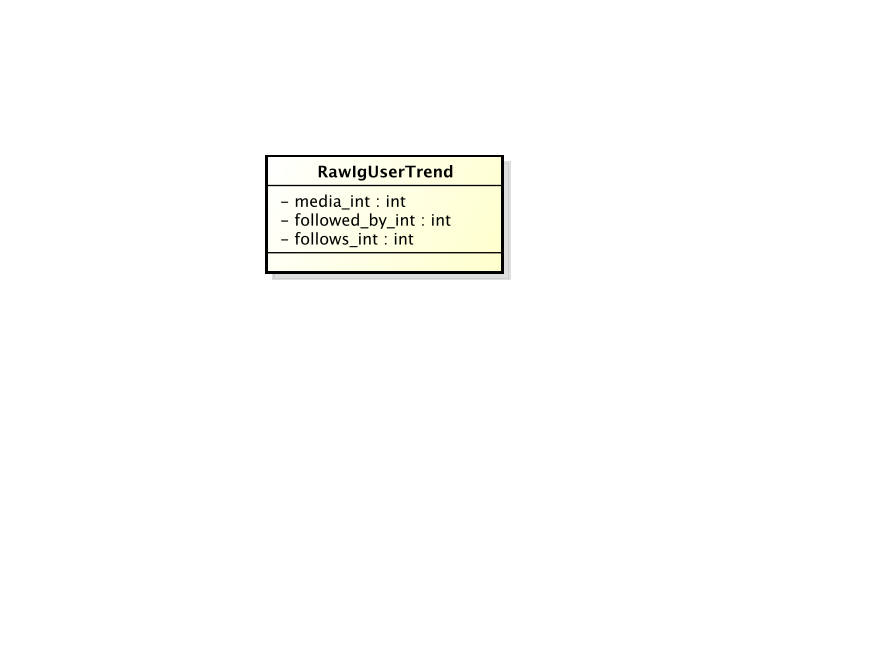
\includegraphics[scale=0.75]{./images/server/classes/db/raw_ig_user_trend.pdf}}
				\caption{Classe - server::db::raw\_data::ig::RawIgUserTrend}
			\end{figure}
			\begin{itemize}
				\item \textbf{Descrizione}: classe che definisce il modello dei dati del trend di un utente Instagram;
				\item \textbf{Utilizzo}: la classe viene utilizzata per memorizzare il numero di media, di followed e follows di una determinata persona. Come per tutti gli oggetti di tipo trend, vengono ricavati i dati fino a 3 giorni prima della creazione dell'oggetto;
				\item \textbf{Classi ereditate}: server::db::raw\_data::AbsRawData
				\item \textbf{Attributi}:
					\begin{itemize}
						\item \textcolor{forestgreen}{\texttt{+ media\_int : int}}
						\begin{description}
							\item \textbf{Descrizione}: numero di media caricati dall'utente su Instagram.
						\end{description}
						\item \textcolor{forestgreen}{\texttt{+ followed\_by\_int : int}}
						\begin{description}
							\item \textbf{Descrizione}: numero di followed dell'utente su Instagram.
						\end{description}
						\item \textcolor{forestgreen}{\texttt{+ follows\_int : int}}
						\begin{description}
							\item \textbf{Descrizione}: numero di following dell'utente su Instagram.
						\end{description}
					\end{itemize}
				\item \textbf{Metodi}: N/A
			\end{itemize}
		% subparagraph server_db_raw_data_ig_rawigusertrend [end]


		\subparagraph{server::db::raw\_data::ig::RawIgHashtag} % (fold)
		\label{subp:server_db_raw_data_ig_rawighashtag}
			\begin{itemize}
				\item \textbf{Descrizione}: classe che definisce il modello dei dati di un hashtag Instagram;
				\item \textbf{Utilizzo}: la classe viene utilizzata per fornire una descrizione minimale dell'hashtag su Instagram. Sebbene tale classe non fornisca metodi o campi dati, risulta molto utile per distinguere un hashtag Instagram da un'altra metrica tramite type checking;
				\item \textbf{Classi ereditate}: server::db::raw\_data::AbsIgRawData
				\item \textbf{Relazioni con altre classi}:
					\begin{itemize}
						\item server::db::raw\_data::ig::RawIgHashtagTrend
						\item server::db::raw\_data::ig::RawIgMedia
					\end{itemize}
				\item \textbf{Attributi}: N/A
				\item \textbf{Metodi}: N/A
			\end{itemize}
		% subparagraph server_db_raw_data_ig_rawighashtag [end]


		\subparagraph{server::db::raw\_data::ig::RawIgHashtagTrend} % (fold)
		\label{subp:server_db_raw_data_ig_rawighashtagtrend}
			\begin{figure}[htbp]
				\centering
				\centerline{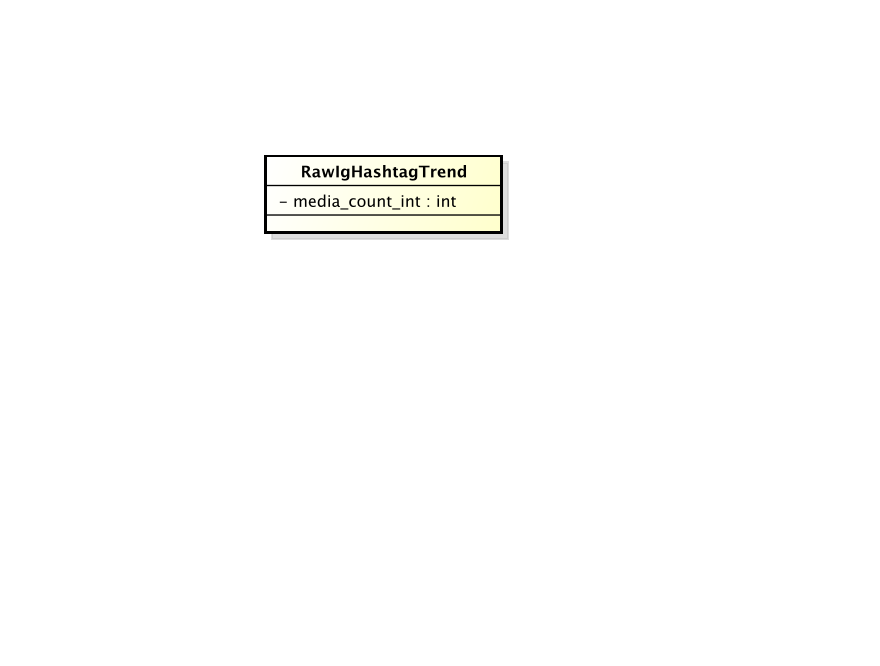
\includegraphics[scale=0.75]{./images/server/classes/db/raw_ig_hashtag_trend.pdf}}
				\caption{Classe - server::db::raw\_data::ig::RawIgHashtagTrend}
			\end{figure}
			\begin{itemize}
				\item \textbf{Descrizione}: classe che definisce il modello dei dati del trend di un hashtag Instagram;
				\item \textbf{Utilizzo}: la classe viene utilizzata per memorizzare il numero di media caricati di un determinato hashtag. Come per tutti gli oggetti di tipo trend, vengono ricavati i dati fino a 3 giorni prima della creazione dell'oggetto;
				\item \textbf{Classi ereditate}: server::db::raw\_data::AbsRawData
				\item \textbf{Attributi}:
					\begin{itemize}
						\item \textcolor{forestgreen}{\texttt{+ media\_count\_int : int}}
						\begin{description}
							\item \textbf{Descrizione}: numero totale di media relativi ad un hashtag su Instagram.
						\end{description}
					\end{itemize}
				\item \textbf{Metodi}: N/A
			\end{itemize}
		% subparagraph server_db_raw_data_ig_rawighashtagtrend [end]


		\subparagraph{server::db::raw\_data::ig::RawIgMedia} % (fold)
		\label{subp:server_db_raw_data_ig_rawigmedia}
			\begin{figure}[htbp]
				\centering
				\centerline{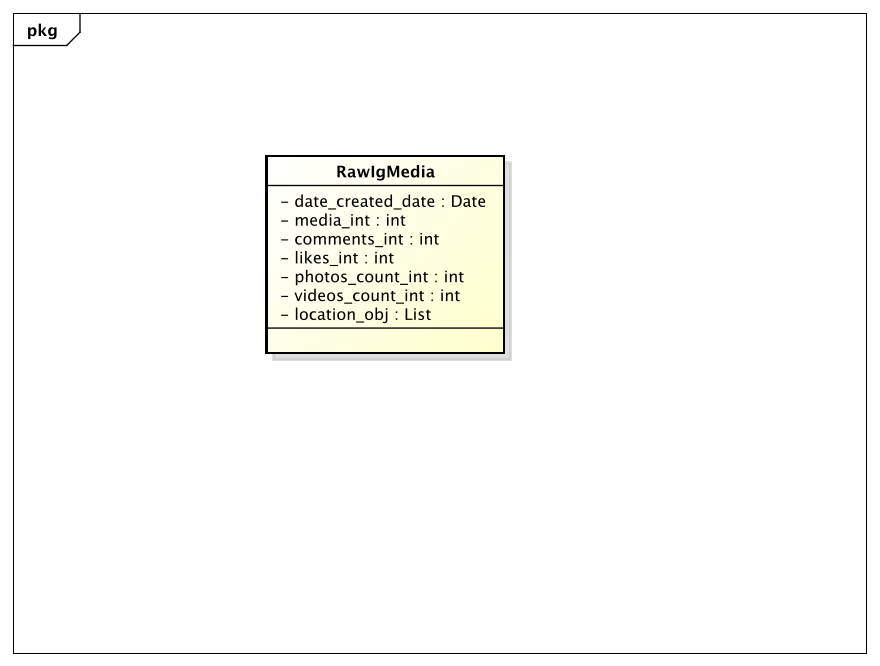
\includegraphics[scale=0.75]{./images/server/classes/db/raw_ig_media.pdf}}
				\caption{Classe - server::db::raw\_data::ig::RawIgMedia}
			\end{figure}
			\begin{itemize}
				\item \textbf{Descrizione}: classe che definisce il modello dei dati di un media relativo ad Instagram;
				\item \textbf{Utilizzo}: la classe viene utilizzata per fornire una descrizione dettagliata del trend dei media relativi ad un utente o un hashtag specifico su Instagram. Come per tutti gli oggetti di tipo trend, vengono ricavati i dati fino a 3 giorni prima della creazione dell'oggetto;
				\item \textbf{Classi ereditate}: server::db::raw\_data::AbsRawData
				\item \textbf{Attributi}:
					\begin{itemize}
						\item \textcolor{forestgreen}{\texttt{+ media\_int : int}}
						\begin{description}
							\item \textbf{Descrizione}: numero di media ricavati.
						\end{description}
						\item \textcolor{forestgreen}{\texttt{+ comments\_int : int}}
						\begin{description}
							\item \textbf{Descrizione}: numero totale dei commenti presenti in tutti i media ricavati.
						\end{description}
						\item \textcolor{forestgreen}{\texttt{+ likes\_int : int}}
						\begin{description}
							\item \textbf{Descrizione}: numero totale dei likes presenti in tutti i media ricavati.
						\end{description}
						\item \textcolor{forestgreen}{\texttt{+ photos\_count\_int : int}}
						\begin{description}
							\item \textbf{Descrizione}: numero totale di media di tipo foto.
						\end{description}
						\item \textcolor{forestgreen}{\texttt{+ videos\_count\_int : int}}
						\begin{description}
							\item \textbf{Descrizione}: numero totale di media di tipo video.
						\end{description}
						\item \textcolor{forestgreen}{\texttt{+ location\_obj : GeoPoint}}
						\begin{description}
							\item \textbf{Descrizione}: localizzazione tramite latitudine e longitudine di un media su Instagram.
						\end{description}
					\end{itemize}
				\item \textbf{Metodi}: N/A
			\end{itemize}
		% subparagraph server_db_raw_data_ig_rawigmedia [end]

\subsubsection{server::db::app\_data} % (fold)
\label{ssub:bdsm_app_server_app_data}


	\begin{figure}[htbp]
		\centering
		\centerline{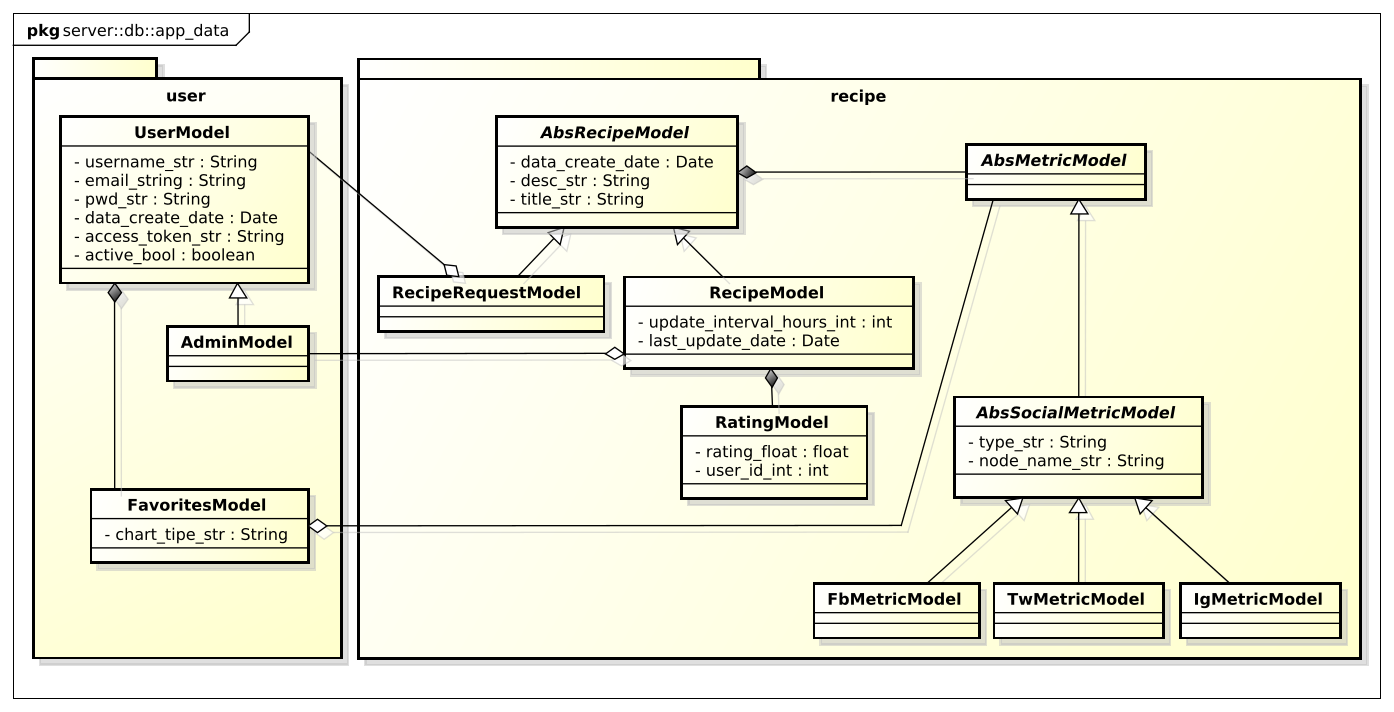
\includegraphics[scale=0.38]{./images/server/app_data.pdf}}
		\caption{Package - server::db::app\_data}
	\end{figure}


	\begin{itemize}
		\item \textbf{Descrizione}: è il package che contiene la definizione dei modelli degli utenti registrati e le loro preferenze. Contiene inoltre il modello delle Recipe che l'amministratore decide di creare;
		\item \textbf{Padre}: server::db
		\item \textbf{Package contenuti}
			\begin{itemize}
				\item server::db::app\_data::user
				\item server::db::app\_data::recipe
			\end{itemize}
	\end{itemize}
	% subsubsection bdsm_app_server_app_data [end]


\subsubsection{server::db::app\_data::user} % (fold)
\label{ssub:bdsm_app_server_app_data_user}

	\begin{itemize}
		\item \textbf{Descrizione}: è il package che contiene la definizione dei modelli degli utenti registrati e le loro preferenze;
		\item \textbf{Padre}: server::db::app\_data
		\item \textbf{Interazione con altri componenti}:
			\begin{itemize}
				\item server::db::app\_data::recipe
			\end{itemize}
	\end{itemize}
	% subsubsection bdsm_app_server_app_data_user [end]


	\paragraph{Classi} % (fold)

		\subparagraph{server::db::app\_data::user::UserModel} % (fold)
		\label{subp:server_db_app_data_user_user_model}
			\begin{figure}[htbp]
				\centering
				\centerline{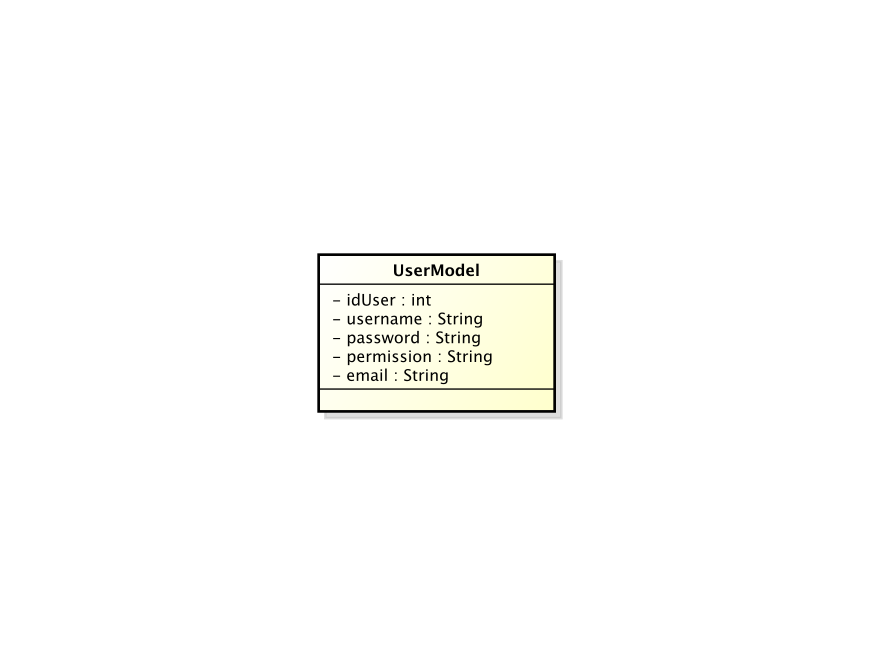
\includegraphics[scale=0.75]{./images/server/classes/db/user_model.pdf}}
				\caption{Classe - server::db::app\_data::user::UserModel}
			\end{figure}
			\begin{itemize}
				\item \textbf{Descrizione}: classe che definisce il modello dei dati degli utenti all'interno della base di dati;
				\item \textbf{Utilizzo}: la classe utilizzata per aggiungere, modificare o eliminare un utente dal database;
				\item \textbf{Relazioni con altre classi}:
					\begin{itemize}
						\item server::db::app\_data::user::FavouritesModel
						\item server::db:::app\_data::user::AdminModel
						\item server::db::app\_data::recipe::RecipeRequestModel
					\end{itemize}
				\item \textbf{Attributi}:
					\begin{itemize}
						\item \textcolor{forestgreen}{\texttt{+ username\_str : String}}
						\begin{description}
							\item \textbf{Descrizione}: lo username dell'utente.
						\end{description}
						\item \textcolor{forestgreen}{\texttt{+ email\_str : String}}
						\begin{description}
							\item \textbf{Descrizione}: l'email dell'utente.
						\end{description}
						\item \textcolor{forestgreen}{\texttt{+ pwd\_str : String}}
						\begin{description}
							\item \textbf{Descrizione}: la password dell'utente.
						\end{description}
						\item \textcolor{forestgreen}{\texttt{+ data\_created\_date : Date}}
						\begin{description}
							\item \textbf{Descrizione}: la data creazione account dell'utente.
						\end{description}
						\item \textcolor{forestgreen}{\texttt{+ access\_token\_str : String}}
						\begin{description}
							\item \textbf{Descrizione}: l'access token utilizzato per i servizi REST.
						\end{description}
						\item \textcolor{forestgreen}{\texttt{+ oauth\_token : String}}
						\begin{description}
							\item \textbf{Descrizione}: il token utilizzato per il processo di autenticazione dell'utente.
						\end{description}
						\item \textcolor{forestgreen}{\texttt{+ active\_bool : boolean}}
						\begin{description}
							\item \textbf{Descrizione}: valore che indica se l'utente attivo nel sistema.
						\end{description}
					\end{itemize}
				\item \textbf{Metodi}: N/A
			\end{itemize}
		% subparagraph server_db_app_data_user_user_model [end]


		\subparagraph{server::db::app\_data::user::AdminModel} % (fold)
		\label{subp:server_db_app_data_user_admin_model}
			\begin{itemize}
				\item \textbf{Descrizione}: classe che definisce il modello dei dati degli utenti amministratori all'interno della base di dati;
				\item \textbf{Utilizzo}: la classe specializza l'utente amministratore. Viene utilizzata esclusivamente per distinguere un amministratore da un utente normale tramite type checking;
				\item \textbf{Classi ereditate}: server::db::app\_data::user::UserModel;
				\item \textbf{Relazioni con altre classi}:
					\begin{itemize}
						\item server::db::app\_data::recipe::RecipeModel
					\end{itemize}
				\item \textbf{Attributi}: N/A
				\item \textbf{Metodi}: N/A
			\end{itemize}
		% subparagraph server_db_app_data_user_admin_model [end]


		\subparagraph{server::db::app\_data::user::FavouritesModel} % (fold)
		\label{subp:server_db_app_data_user_favorites}
			\begin{figure}[htbp]
				\centering
				\centerline{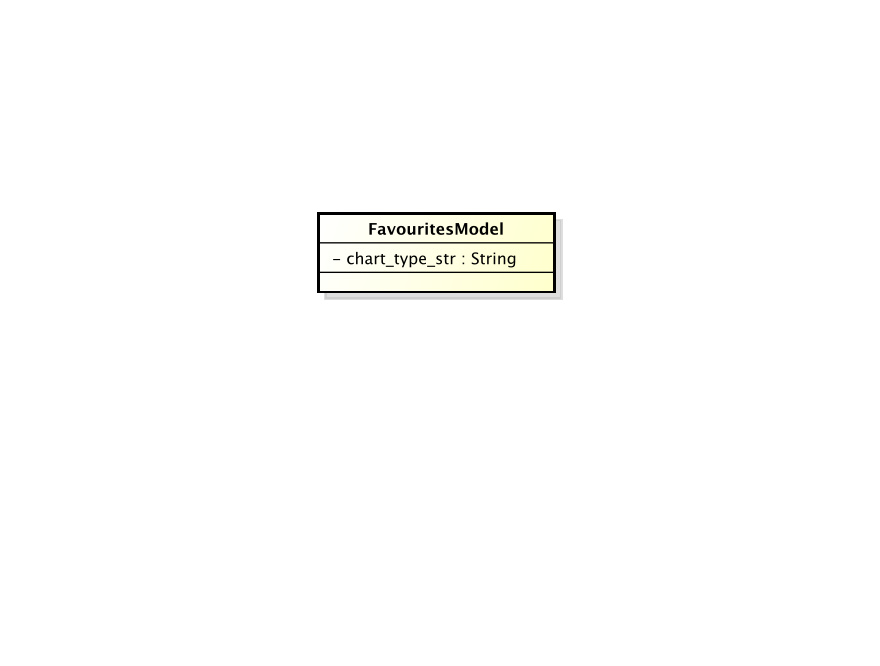
\includegraphics[scale=0.75]{./images/server/classes/db/favourites_model.pdf}}
				\caption{Classe - server::db::app\_data::user::FavouritesModel}
			\end{figure}
			\begin{itemize}
				\item \textbf{Descrizione}: classe che definisce il modello dei dati relativo ai preferiti dell'utente;
				\item \textbf{Utilizzo}: la classe viene utilizzata per memorizzare e ricavare le View preferite relative ad un utente.
				\item \textbf{Relazioni con altre classi}:
					\begin{itemize}
						\item server::db::app\_data::recipe::AbsMetricModel
					\end{itemize}
				\item \textbf{Attributi}:
					\begin{itemize}
						\item \textcolor{forestgreen}{\texttt{chart\_type\_str : String}}
						\begin{description}
							\item \textbf{Descrizione}: tipo di grafico scelto dall'utente e salvato nei preferiti.
						\end{description}
					\end{itemize}
				\item \textbf{Metodi}: N/A
			\end{itemize}
		% subparagraph server_db_app_data_user_favorites [end]


\subsubsection{server::db::app\_data::recipe} % (fold)
\label{ssub:bdsm_app_server_app_data_recipe}

	\begin{itemize}
		\item \textbf{Descrizione}: è il package che contiene la definizione dei modelli delle Recipe che l'amministratore decide di creare;
		\item \textbf{Padre}: server::db::app\_data
		\item \textbf{Interazione con altri componenti}:
			\begin{itemize}
				\item server::db::app\_data::user
			\end{itemize}
	\end{itemize}
	% subsubsection bdsm_app_server_app_data_recipe [end]


	\paragraph{Classi} % (fold)

		\subparagraph{server::db::app\_data::recipe::AbsRecipeModel} % (fold)
		\label{subp:server_db_app_data_recipe_absrecipemodel}
			\begin{figure}[htbp]
				\centering
				\centerline{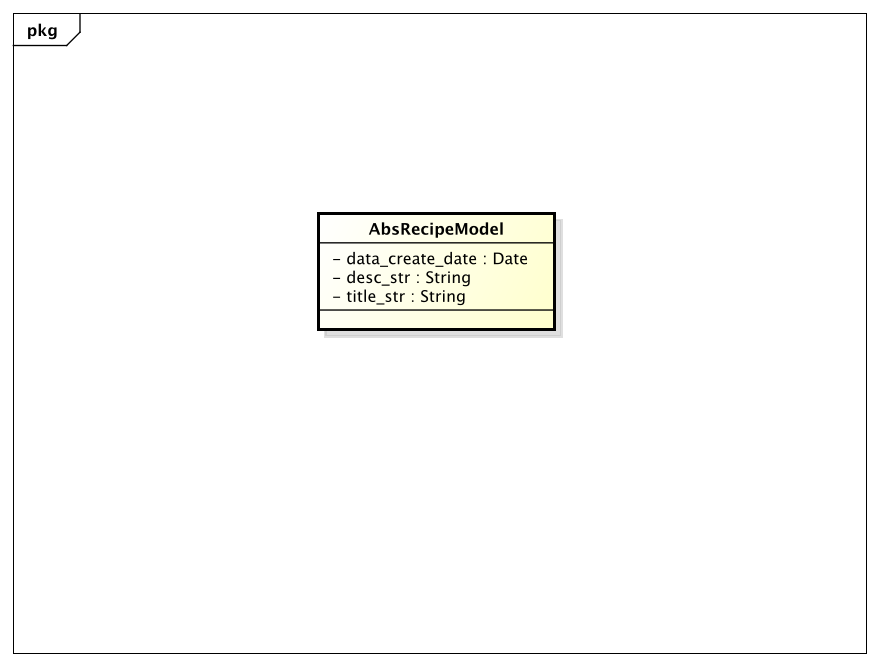
\includegraphics[scale=0.75]{./images/server/classes/db/abs_recipe_model.pdf}}
				\caption{Classe - server::db::app\_data::recipe::AbsRecipeModel}
			\end{figure}
			\begin{itemize}
				\item \textbf{Descrizione}: classe astratta che rappresenta un modello comune per Recipe e richiesta di aggiunta Recipe;
				\item \textbf{Utilizzo}: la classe mantiene l'estensibilità per eventuali nuovi tipi di Recipe;
				\item \textbf{Relazioni con altre classi}:
					\begin{itemize}
						\item server::db::app\_data::recipe::RecipeModel
						\item server::db::app\_data::recipe::RecipeRequestModel
						\item server::db::app\_data::recipe::AbsMetricModel
					\end{itemize}
				\item \textbf{Attributi}:
					\begin{itemize}
						\item \textcolor{forestgreen}{\texttt{data\_create\_date : Date}}
						\begin{description}
							\item \textbf{Descrizione}: data di creazione della Recipe.
						\end{description}
						\item \textcolor{forestgreen}{\texttt{desc\_str : String}}
						\begin{description}
							\item \textbf{Descrizione}: descrizione dettagliata dell Recipe.
						\end{description}
						\item \textcolor{forestgreen}{\texttt{title\_str : String}}
						\begin{description}
							\item \textbf{Descrizione}: titolo della Recipe.
						\end{description}
					\end{itemize}
				\item \textbf{Metodi}: N/A
			\end{itemize}
		% subparagraph server_db_app_data_recipe_absrecipemodel [end]


		\subparagraph{server::db::app\_data::recipe::RecipeRequestModel} % (fold)
		\label{subp:server_db_app_data_recipe_reciperequestmodel}
			\begin{itemize}
				\item \textbf{Descrizione}: classe che definisce il modello dei dati per la richiesta di aggiunta Recipe;
				\item \textbf{Utilizzo}: la classe specializza la richiesta identificandone l'utente tramite il rapporto parent-child delle classi di Google Datastore;
				\item \textbf{Classi ereditate}: server::db::app\_data::recipe::AbsRecipeModel
				\item \textbf{Attributi}: N/A
				\item \textbf{Metodi}: N/A
			\end{itemize}
		% subparagraph server_db_app_data_recipe_reciperequestmodel [end]


		\subparagraph{server::db::app\_data::recipe::RecipeModel} % (fold)
		\label{subp:server_db_app_data_recipe_recipemodel}
			\begin{figure}[htbp]
				\centering
				\centerline{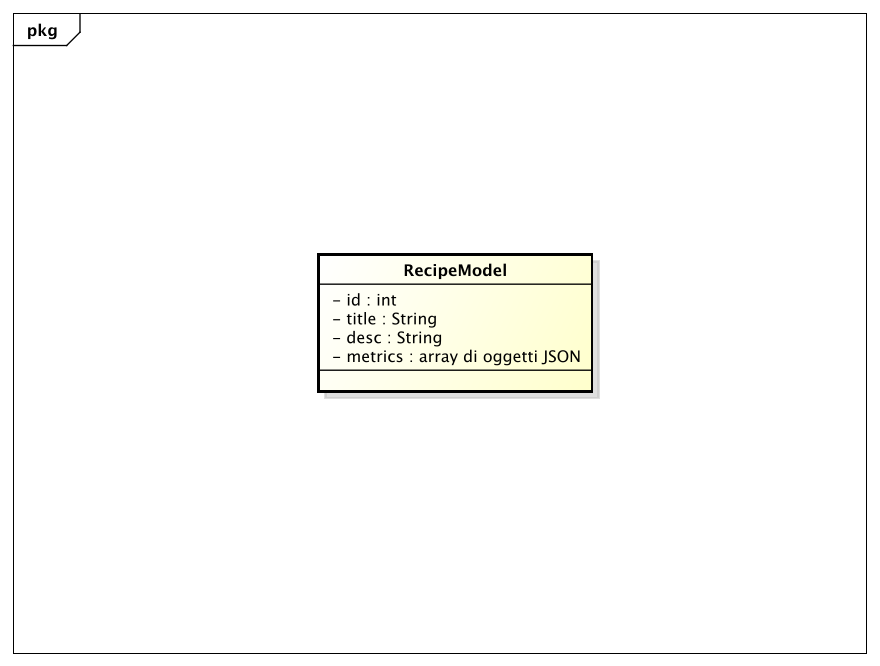
\includegraphics[scale=0.75]{./images/server/classes/db/recipe_model.pdf}}
				\caption{Classe - server::db::app\_data::recipe::RecipeModel}
			\end{figure}
			\begin{itemize}
				\item \textbf{Descrizione}: classe che definisce il modello dei dati relativo ad una Recipe;
				\item \textbf{Utilizzo}: la classe specializza la ricetta. Vengono forniti i campi dati per il possibile incremento temporale dei dati;
				\item \textbf{Classi ereditate}: server::db::app\_data::recipe::AbsRecipeModel
				\item \textbf{Relazioni con altre classi}:
					\begin{itemize}
						\item server::db::app\_data::recipe::RatingModel
					\end{itemize}
				\item \textbf{Attributi}:
					\begin{itemize}
						\item \textcolor{forestgreen}{\texttt{+ update\_interval\_hours\_int : int}}
						\begin{description}
							\item \textbf{Descrizione}: intervallo di tempo per la schedulazione dell'update della Recipe.
						\end{description}
						\item \textcolor{forestgreen}{\texttt{+ last\_update\_date : Date}}
						\begin{description}
							\item \textbf{Descrizione}: data dell'ultimo processo di update Recipe.
						\end{description}
					\end{itemize}
				\item \textbf{Metodi}: N/A
			\end{itemize}
		% subparagraph server_db_app_data_recipe_recipemodel [end]

		\subparagraph{server::db::app\_data::recipe::RatingModel} % (fold)
		\label{subp:server_db_app_data_recipe_recipemodel}
			\begin{figure}[htbp]
				\centering
				\centerline{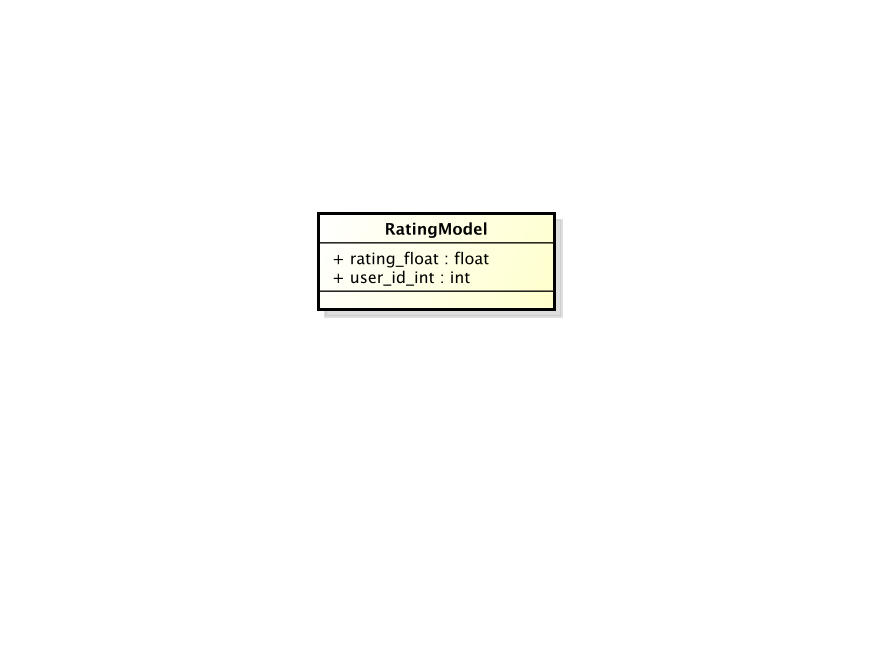
\includegraphics[scale=0.75]{./images/server/classes/db/rating_model.pdf}}
				\caption{Classe - server::db::app\_data::recipe::RatingModel}
			\end{figure}
			\begin{itemize}
				\item \textbf{Descrizione}: classe che rappresenta il modello del rating di una Recipe;
				\item \textbf{Utilizzo}: viene utilizzata per risalire al voto di ogni utente per una determinata Recipe;
				\item \textbf{Attributi}:
					\begin{itemize}
						\item \textcolor{forestgreen}{\texttt{+ rating\_float : float}}
						\begin{description}
							\item \textbf{Descrizione}: punteggio gradimento relativo alla Recipe.
						\end{description}
						\item \textcolor{forestgreen}{\texttt{+ user\_id\_int : int}}
					\end{itemize}
					\begin{description}
							\item \textbf{Descrizione}: identificativo dell'utente votante.
						\end{description}
				\item \textbf{Metodi}: N/A
			\end{itemize}
		% subparagraph server_db_app_data_recipe_recipemodel [end]


		\subparagraph{server::db::app\_data::recipe::AbsMetricModel} % (fold)
		\label{subp:server_db_app_data_recipe_absmetricmodel}
			\begin{itemize}
				\item \textbf{Descrizione}: classe che definisce il modello dei dati di una metrica contenuta in una Ricetta;
				\item \textbf{Utilizzo}: la classe rappresenta il modello dei dati di una metrica generale;
				\item \textbf{Relazioni con altre classi}:
					\begin{itemize}
						\item server::db::app\_data::recipe::AbsSocialMetricModel
					\end{itemize}
				\item \textbf{Attributi}: N/A
				\item \textbf{Metodi}: N/A
			\end{itemize}
		% subparagraph server_db_app_data_recipe_absmetricmodel [end]


		\subparagraph{server::db::app\_data::recipe::AbsSocialMetricModel} % (fold)
		\label{subp:server_db_app_data_recipe_abssocialmetricmodel}
			\begin{figure}[htbp]
				\centering
				\centerline{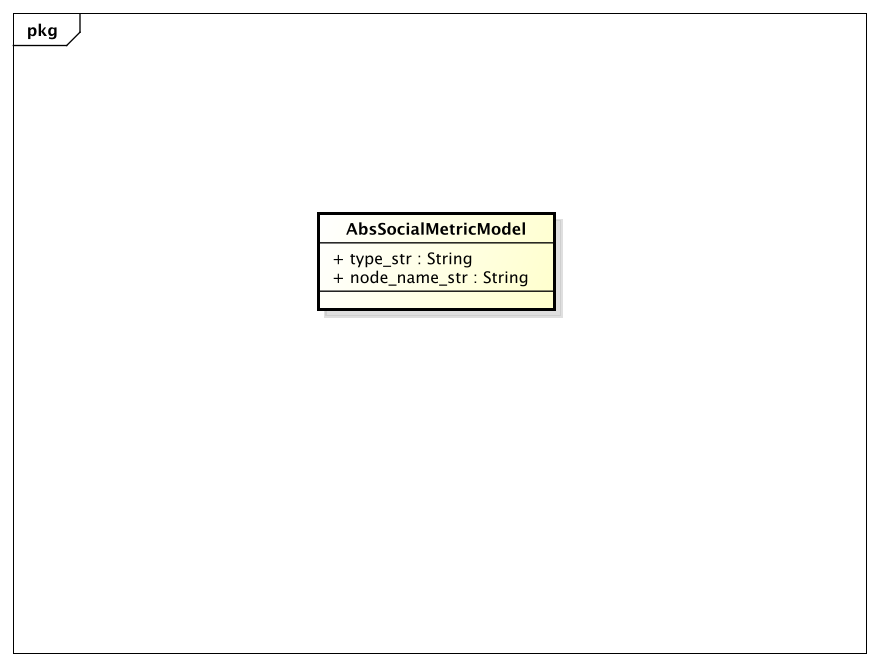
\includegraphics[scale=0.75]{./images/server/classes/db/abs_social_metric_model.pdf}}
				\caption{Classe - server::db::app\_data::recipe::AbsSocialMetricModel}
			\end{figure}
			\begin{itemize}
				\item \textbf{Descrizione}: classe che definisce il modello dei dati delle metriche relative ai social media;
				\item \textbf{Utilizzo}: la classe rappresenta il modello di una metrica relativa ad un social network fornendo il tipo di metrica e il suo identificativo;
				\item \textbf{Classi ereditate}: server::db::app\_data::recipe::AbsMetricModel
				\item \textbf{Relazioni con altre classi}:
					\begin{itemize}
						\item server::db::app\_data::recipe::FbMetricModel
						\item server::db::app\_data::recipe::IgMetricModel
						\item server::db::app\_data::recipe::TwMetricModel
					\end{itemize}
				\item \textbf{Attributi}:
					\begin{itemize}
						\item \textcolor{forestgreen}{\texttt{+ type\_str : String}}
						\begin{description}
							\item \textbf{Descrizione}: tipo della metrica (pagina, evento, hashtag).
						\end{description}
						\item \textcolor{forestgreen}{\texttt{+ node\_name\_str : String}}
						\begin{description}
							\item \textbf{Descrizione}: nome identificativo della metrica.
						\end{description}
					\end{itemize}
				\item \textbf{Metodi}: N/A
			\end{itemize}
		% subparagraph server_db_app_data_recipe_abssocialmetricmodel [end]


		\subparagraph{server::db::app\_data::recipe::FbMetricModel} % (fold)
		\label{subp:server_db_app_data_recipe_fbmetricmodel}
			\begin{itemize}
				\item \textbf{Descrizione}: classe che definisce il modello dei dati delle metriche relative a Facebook;
				\item \textbf{Utilizzo}: viene utilizzata esclusivamente per offrire una distinzione di tipo per le metriche relative a Facebook rispetto ai restanti social network;
				\item \textbf{Classi ereditate}: server::db::app\_data::recipe::AbsSocialMetricModel;
				\item \textbf{Attributi}: N/A
				\item \textbf{Metodi}: N/A
			\end{itemize}
		% subparagraph server_db_app_data_recipe_fbmetricmodel [end]


		\subparagraph{server::db::app\_data::recipe::IgMetricModel} % (fold)
		\label{subp:server_db_app_data_recipe_igmetricmodel}
			\begin{itemize}
				\item \textbf{Descrizione}: classe che definisce il modello dei dati delle metriche relative a Instagram;
				\item \textbf{Utilizzo}: viene utilizzata esclusivamente per offrire una distinzione di tipo per le metriche relative a Instagram rispetto ai restanti social network;
				\item \textbf{Classi ereditate}: server::db::app\_data::recipe::AbsSocialMetricModel;
				\item \textbf{Attributi}: N/A
				\item \textbf{Metodi}: N/A
			\end{itemize}
		% subparagraph server_db_app_data_recipe_igmetricmodel [end]


		\subparagraph{server::db::app\_data::recipe::TwMetricModel} % (fold)
		\label{subp:server_db_app_data_recipe_twmetricmodel}
			\begin{itemize}
				\item \textbf{Descrizione}: classe che definisce il modello dei dati delle metriche relative a Twitter;
				\item \textbf{Utilizzo}: viene utilizzata esclusivamente per offrire una distinzione di tipo per le metriche relative a Twitter rispetto ai restanti social network;
				\item \textbf{Classi ereditate}: server::db::app\_data::recipe::AbsSocialMetricModel;
				\item \textbf{Attributi}: N/A
				\item \textbf{Metodi}: N/A
			\end{itemize}
		% subparagraph server_db_app_data_recipe_twmetricmodel [end]
 \clearpage \newpage
  % END PACKAGE DB

  % PACKAGE PROCESSOR
  % =================================================================================================
% File:			server_tier/processor.tex
% Description:	Definisce la sezione relativa al back-end dell'applicazione
% Created:		2015-04-07
% Author:		Cusinato Giacomo
% Email:		cusinato.giacomo@mashup-unipd.it
% =================================================================================================
% Modification History:
% Version		Modifier Date		Change											Author
% 0.0.1
% =================================================================================================

% CONTENUTO DEL CAPITOLO


\subsubsection{bdsm\_app::server::processor} % (fold)
\label{ssub:bdsm_app_server_processor}
[TO DO] (diagramma) \newline \newline

\begin{itemize}
  \item \textbf{Descrizione}: [TO DO];
  \item \textbf{Padre}: [TO DO] (qualora presente);
  \item \textbf{Package contenuti}: [TO DO] (qualora presente);
  \item \textbf{Interazione con altri componenti}: [TO DO];
\end{itemize}
% subsubsection
 \clearpage \newpage
  % END PACKAGE PROCESSOR

  % PACKAGE MINER
  % =================================================================================================
% File:			server_tier/miner.tex
% Description:	Definisce la sezione relativa al back-end dell'applicazione
% Created:		2015-04-07
% Author:		Cusinato Giacomo
% Email:		cusinato.giacomo@mashup-unipd.it
% =================================================================================================
% Modification History:
% Version		Modifier Date		Change											Author
% 0.0.1
% =================================================================================================

% CONTENUTO DEL CAPITOLO


\subsubsection{bdsm\_app::server::miner} % (fold)
\label{ssub:bdsm_app_server_miner}
[TO DO] (diagramma) \newline \newline

\begin{itemize}
  \item \textbf{Descrizione}: è il package che contiene tutte le classi con i metodi per prelevare i dati dai social network e per salvarli nel database;
  \item \textbf{Padre}: server;
  \item \textbf{Package contenuti}:
  	\begin{itemize}
  		\item fb;
  		\item ig;
  		\item tw;
  	\end{itemize}
  \item \textbf{Interazione con altri componenti}:
  	\begin{itemize}
  		\item server::processor
  		\item server::database
  	\end{itemize}
\end{itemize}

\paragraph{Classi} % (fold)
		\subparagraph{server::miner::MinerScheduler} % (fold)
		\label{subp:server_miner_MinerScheduler}
			\begin{itemize}
				\item \textbf{Descrizione}:
				\item \textbf{Utilizzo}: 
				\item \textbf{Relazioni con altre classi}:
					\begin{itemize}
						\item 
					\end{itemize}
			\end{itemize}
		% subparagraph server_miner_MinerScheduler
		
		\subparagraph{server::miner::AbsCounter} % (fold)
		\label{subp:server_miner_AbsCounter}
			\begin{itemize}
				\item \textbf{Descrizione}: 
				\item \textbf{Utilizzo}: 
				\item \textbf{Relazioni con altre classi}:
					\begin{itemize}
						\item 
					\end{itemize}
			\end{itemize}
		% subparagraph server_miner_AbsCounter
		
		\subparagraph{server::miner::AbsFetcher} % (fold)
		\label{subp:server_miner_AbsFetcher}
			\begin{itemize}
				\item \textbf{Descrizione}: 
				\item \textbf{Utilizzo}: 
				\item \textbf{Relazioni con altre classi}:
					\begin{itemize}
						\item 
					\end{itemize}
			\end{itemize}
		% subparagraph server_miner_AbsFetcher
		
\subsubsection{bdsm\_app::server::miner::fb} % (fold)
\label{ssub:bdsm_app_server_miner_fb}
[TO DO] (diagramma) \newline \newline

\begin{itemize}
  \item \textbf{Descrizione}:
  \item \textbf{Padre}:
  \item \textbf{Package contenuti}:
  	\begin{itemize}
  		\item
  	\end{itemize}
  \item \textbf{Interazione con altri componenti}:
  	\begin{itemize}
  		\item  	
  	\end{itemize}
\end{itemize}	

	\paragraph{Classi} % (fold)
		\subparagraph{server::miner::fb::AbsFbFetcher} % (fold)
		\label{subp:server_miner_fb_AbsFbFetcher}
			\begin{itemize}
				\item \textbf{Descrizione}:
				\item \textbf{Utilizzo}: 
				\item \textbf{Relazioni con altre classi}:
					\begin{itemize}
						\item 
					\end{itemize}
			\end{itemize}
	% subparagraph server_miner_fb_AbsFbFetcher
	
		\subparagraph{server::miner::fb::FbPageFetcher} % (fold)
		\label{subp:server_miner_fb_FbPageFetcher}
			\begin{itemize}
				\item \textbf{Descrizione}:
				\item \textbf{Utilizzo}: 
				\item \textbf{Relazioni con altre classi}:
					\begin{itemize}
						\item 
					\end{itemize}
			\end{itemize}
	% subparagraph server_miner_fb_FbPageFetcher
	
		\subparagraph{server::miner::fb::FbEventFetcher} % (fold)
		\label{subp:server_miner_fb_FbEventFetcher}
			\begin{itemize}
				\item \textbf{Descrizione}:
				\item \textbf{Utilizzo}: 
				\item \textbf{Relazioni con altre classi}:
					\begin{itemize}
						\item 
					\end{itemize}
			\end{itemize}
	% subparagraph server_miner_fb_FbEventFetcher
	
		\subparagraph{server::miner::fb::AbsFbCounter} % (fold)
		\label{subp:server_miner_fb_AbsFbCounter}
			\begin{itemize}
				\item \textbf{Descrizione}:
				\item \textbf{Utilizzo}: 
				\item \textbf{Relazioni con altre classi}:
					\begin{itemize}
						\item 
					\end{itemize}
			\end{itemize}
	% subparagraph server_miner_fb_AbsFbCounter
	
		\subparagraph{server::miner::fb::AttendingCounter} % (fold)
		\label{subp:server_miner_fb_AttendingCounter}
			\begin{itemize}
				\item \textbf{Descrizione}:
				\item \textbf{Utilizzo}: 
				\item \textbf{Relazioni con altre classi}:
					\begin{itemize}
						\item 
					\end{itemize}
			\end{itemize}
	% subparagraph server_miner_fb_AttendingCounter
	
		\subparagraph{server::miner::fb::MaybeCounter} % (fold)
		\label{subp:server_miner_fb_MaybeCounter}
			\begin{itemize}
				\item \textbf{Descrizione}:
				\item \textbf{Utilizzo}: 
				\item \textbf{Relazioni con altre classi}:
					\begin{itemize}
						\item 
					\end{itemize}
			\end{itemize}
	% subparagraph server_miner_fb_MaybeCounter
	
	\subparagraph{server::miner::fb::InvitedCounter} % (fold)
		\label{subp:server_miner_fb_InvitedCunter}
			\begin{itemize}
				\item \textbf{Descrizione}:
				\item \textbf{Utilizzo}: 
				\item \textbf{Relazioni con altre classi}:
					\begin{itemize}
						\item 
					\end{itemize}
			\end{itemize}
	% subparagraph server_miner_fb_InvitedCounter

	\subparagraph{server::miner::fb::RefusedCounter} % (fold)
		\label{subp:server_miner_fb_RefusedCounter}
			\begin{itemize}
				\item \textbf{Descrizione}:
				\item \textbf{Utilizzo}: 
				\item \textbf{Relazioni con altre classi}:
					\begin{itemize}
						\item 
					\end{itemize}
			\end{itemize}
	% subparagraph server_miner_fb_RefusedCounter
	
	\subparagraph{server::miner::fb::PostCounter} % (fold)
		\label{subp:server_miner_fb_PostCounter}
			\begin{itemize}
				\item \textbf{Descrizione}:
				\item \textbf{Utilizzo}: 
				\item \textbf{Relazioni con altre classi}:
					\begin{itemize}
						\item 
					\end{itemize}
			\end{itemize}
	% subparagraph server_miner_fb_PostCounter
	
	\subparagraph{server::miner::fb::CommentCounter} % (fold)
		\label{subp:server_miner_fb_CommentCounter}
			\begin{itemize}
				\item \textbf{Descrizione}:
				\item \textbf{Utilizzo}: 
				\item \textbf{Relazioni con altre classi}:
					\begin{itemize}
						\item 
					\end{itemize}
			\end{itemize}
	% subparagraph server_miner_fb_CommentCounter
	
	\subparagraph{server::miner::fb::LikeCounter} % (fold)
		\label{subp:server_miner_fb_LikeCounter}
			\begin{itemize}
				\item \textbf{Descrizione}:
				\item \textbf{Utilizzo}: 
				\item \textbf{Relazioni con altre classi}:
					\begin{itemize}
						\item 
					\end{itemize}
			\end{itemize}
	% subparagraph server_miner_fb_LikeCounter

\subsubsection{bdsm\_app::server::miner::tw} % (fold)
\label{ssub:bdsm_app_server_miner_tw}
[TO DO] (diagramma) \newline \newline

\begin{itemize}
  \item \textbf{Descrizione}:
  \item \textbf{Padre}:
  \item \textbf{Package contenuti}:
  	\begin{itemize}
  		\item
  	\end{itemize}
  \item \textbf{Interazione con altri componenti}:
  	\begin{itemize}
  		\item  	
  	\end{itemize}
\end{itemize}	

	\paragraph{Classi} % (fold)
	\subparagraph{server::miner::tw::AbsTwFetcher} % (fold)
		\label{subp:server_miner_tw_AbsTwFetcher}
			\begin{itemize}
				\item \textbf{Descrizione}:
				\item \textbf{Utilizzo}: 
				\item \textbf{Relazioni con altre classi}:
					\begin{itemize}
						\item 
					\end{itemize}
			\end{itemize}
		% subparagraph server_miner_tw_AbsTwFetcher
		
	\subparagraph{server::miner::tw::TwHashtagFetcher} % (fold)
		\label{subp:server_miner_tw_TwHashtagFetcher}
			\begin{itemize}
				\item \textbf{Descrizione}:
				\item \textbf{Utilizzo}: 
				\item \textbf{Relazioni con altre classi}:
					\begin{itemize}
						\item 
					\end{itemize}
			\end{itemize}
		% subparagraph server_miner_tw_TwHashtagFetcher
		
	\subparagraph{server::miner::tw::TwUserFetcher} % (fold)
		\label{subp:server_miner_tw_TwUserFetcher}
			\begin{itemize}
				\item \textbf{Descrizione}:
				\item \textbf{Utilizzo}: 
				\item \textbf{Relazioni con altre classi}:
					\begin{itemize}
						\item 
					\end{itemize}
			\end{itemize}
		% subparagraph server_miner_tw_TwUserFetcher
		
	\subparagraph{server::miner::tw::AbsTwCounter} % (fold)
		\label{subp:server_miner_tw_AbsTwCounter}
			\begin{itemize}
				\item \textbf{Descrizione}:
				\item \textbf{Utilizzo}: 
				\item \textbf{Relazioni con altre classi}:
					\begin{itemize}
						\item 
					\end{itemize}
			\end{itemize}
		% subparagraph server_miner_tw_AbsTwCounter
		
	\subparagraph{server::miner::tw::UserTweetCounter} % (fold)
		\label{subp:server_miner_tw_UserTweetCounter}
			\begin{itemize}
				\item \textbf{Descrizione}:
				\item \textbf{Utilizzo}: 
				\item \textbf{Relazioni con altre classi}:
					\begin{itemize}
						\item 
					\end{itemize}
			\end{itemize}
		% subparagraph server_miner_tw_UserTweetCounter
		
		
	\subparagraph{server::miner::tw::HashtagTweetCounter} % (fold)
		\label{subp:server_miner_tw_HashtagTweetCounter}
			\begin{itemize}
				\item \textbf{Descrizione}:
				\item \textbf{Utilizzo}: 
				\item \textbf{Relazioni con altre classi}:
					\begin{itemize}
						\item 
					\end{itemize}
			\end{itemize}
		% subparagraph server_miner_tw_HashtagTweetCounter

\subsubsection{bdsm\_app::server::miner::ig} % (fold)
\label{ssub:bdsm_app_server_miner_ig}
[TO DO] (diagramma) \newline \newline

\begin{itemize}
  \item \textbf{Descrizione}:
  \item \textbf{Padre}:
  \item \textbf{Package contenuti}:
  	\begin{itemize}
  		\item
  	\end{itemize}
  \item \textbf{Interazione con altri componenti}:
  	\begin{itemize}
  		\item  	
  	\end{itemize}
\end{itemize}	

	\paragraph{Classi} % (fold)
	\subparagraph{server::miner::ig::AbsIgFetcher} % (fold)
		\label{subp:server_miner_tw_AbsIgFetcher}
			\begin{itemize}
				\item \textbf{Descrizione}:
				\item \textbf{Utilizzo}: 
				\item \textbf{Relazioni con altre classi}:
					\begin{itemize}
						\item 
					\end{itemize}
			\end{itemize}
		% subparagraph server_miner_tw_AbsIgFetcher		

	\subparagraph{server::miner::ig::IgUserFetcher} % (fold)
		\label{subp:server_miner_tw_IgUserFetcher}
			\begin{itemize}
				\item \textbf{Descrizione}:
				\item \textbf{Utilizzo}: 
				\item \textbf{Relazioni con altre classi}:
					\begin{itemize}
						\item 
					\end{itemize}
			\end{itemize}
		% subparagraph server_miner_tw_IgUserFetcher		
		
	\subparagraph{server::miner::ig::IgHashtagFetcher} % (fold)
		\label{subp:server_miner_tw_IgHashtagFetcher}
			\begin{itemize}
				\item \textbf{Descrizione}:
				\item \textbf{Utilizzo}: 
				\item \textbf{Relazioni con altre classi}:
					\begin{itemize}
						\item 
					\end{itemize}
			\end{itemize}
		% subparagraph server_miner_tw_IgHashtagFetcher		
		
	\subparagraph{server::miner::ig::AbsIgCounter} % (fold)
		\label{subp:server_miner_tw_AbsIgCounter}
			\begin{itemize}
				\item \textbf{Descrizione}:
				\item \textbf{Utilizzo}: 
				\item \textbf{Relazioni con altre classi}:
					\begin{itemize}
						\item 
					\end{itemize}
			\end{itemize}
		% subparagraph server_miner_tw_AbsIgCounter		
		
		
	\subparagraph{server::miner::ig::MediaCounter} % (fold)
		\label{subp:server_miner_tw_MediaCounter}
			\begin{itemize}
				\item \textbf{Descrizione}:
				\item \textbf{Utilizzo}: 
				\item \textbf{Relazioni con altre classi}:
					\begin{itemize}
						\item 
					\end{itemize}
			\end{itemize}
		% subparagraph server_miner_tw_MediaCounter		

		
% subsubsection
 \clearpage \newpage
  % END PACKAGE MINER

  % PACKAGE ENDPOINTS
  % =================================================================================================
% File:			server_tier/endpoints.tex
% Description:	Definisce la sezione relativa al back-end dell'applicazione
% Created:		2015-04-07
% Author:		Cusinato Giacomo
% Email:		cusinato.giacomo@mashup-unipd.it
% =================================================================================================
% Modification History:
% Version		Modifier Date		Change											Author
% 0.0.1
% =================================================================================================

% CONTENUTO DEL CAPITOLO


\subsubsection{bdsm\_app::server::endpoints} % (fold)
\label{ssub:bdsm_app_server_endpoints}
[TO DO] (diagramma) \newline \newline

\begin{itemize}
  \item \textbf{Descrizione}: è il package che contiene tutte le classi utili ad effettuare le chiamate REST e a ritornare i risultati;
  \item \textbf{Padre}: server
  \item \textbf{Package contenuti}:
  	\begin{itemize}
  		\item server::endpoints::api
  		\item server::endpoints::resp
	\end{itemize}
  \item \textbf{Interazione con altri componenti}:
  	\begin{itemize}
  		\item server::processor
  		\item server::miner
  		\item server::db
	\end{itemize}
\end{itemize}
% subsubsection

\subsubsection{bdsm\_app::server::endpoints::api} % (fold)
\label{ssub:bdsm_app_server_endpoints_api}
[TO DO] (diagramma) \newline \newline

\begin{itemize}
  \item \textbf{Descrizione}: è il package che definisce i servizi REST offerti dall'applicazione e utilizzati dal client;
  \item \textbf{Padre}: server::endpoints
  \item \textbf{Package contenuti}:
  	\begin{itemize}
  		\item server::endpoints::api::public
  		\item server::endpoints::api::private
	\end{itemize}
  \item \textbf{Interazione con altri componenti}:
  	\begin{itemize}
  		\item client::model::services
  		\item server::processor
  		\item server::db
	\end{itemize}
\end{itemize}
% subsubsection

\subsubsection{bdsm\_app::server::endpoints::api::public} % (fold)
\label{ssub:bdsm_app_server_endpoints_api_public}
[TO DO] (diagramma) \newline \newline

\begin{itemize}
  \item \textbf{Descrizione}: è il package contenente le componenti che contengono i servizi REST pubblici;
  \item \textbf{Padre}: server::endpoints::api
  \item \textbf{Interazione con altri componenti}:
  	\begin{itemize}
        \item server::processor
    \end{itemize}
\end{itemize}
% subsubsection

	\paragraph{Classi} % (fold)

    \subparagraph{bdsm\_app::server::endpoints::api::public::RecipeApi} % (fold)
    \label{subp:bdsm_app_server_endpoints_api_public_recipeapi}
    \begin{itemize}
      \item \textbf{Descrizione}: classe utilizzata dal client per ricavare la lista delle Recipe e delle metriche;
      \item \textbf{Utilizzo}: i suoi metodi vengono invocati quando viene richiesto dal client di recuperare la lista delle Recipe e delle metriche;
      \item \textbf{Relazioni con altre classi}:
        \begin{itemize}
          \item server::endpoints::resp::public::MetricListResponse;
          \item server::endpoints::resp::private::RecipeListResponse;
        \end{itemize}
      \end{itemize}
    % subparagraph bdsm_app_server_endpoints_api_public_recipeapi (end)
    
    \subparagraph{bdsm\_app::server::endpoints::api::public::FbMetricsApi} % (fold)
    \label{subp:bdsm_app_server_endpoints_api_public_fbmetricsapi}
    \begin{itemize}
      \item \textbf{Descrizione}: classe utilizzata dal client per ottenere i dati relativi ad una metrica di Facebook;
      \item \textbf{Utilizzo}: i suoi metodi vengono invocati quando viene richiesto dal client dei dati relativi ad una pagina o ad un evento di Facebook;
      \item \textbf{Relazioni con altre classi}:
        \begin{itemize}
          \item server::endpoints::resp::public::fb::PageResponse
          \item server::endpoints::resp::public::fb::PageTrendListResponse
          \item server::endpoints::resp::public::fb::PostListResponse
          \item server::endpoints::resp::public::fb::EventResponse
          \item server::endpoints::resp::public::fb::EventTrendListResponse
        \end{itemize}
      \end{itemize}
    % subparagraph bdsm_app_server_endpoints_api_public_fbmetricsapi (end)
    
    \subparagraph{bdsm\_app::server::endpoints::api::public::TwMetricsApi} % (fold)
    \label{subp:bdsm_app_server_endpoints_api_public_twmetricsapi}
    \begin{itemize}
      \item \textbf{Descrizione}: classe utilizzata dal client per ottenere i dati relativi ad una metrica di Twitter;
      \item \textbf{Utilizzo}: i suoi metodi vengono invocati quando viene richiesto dal client dei dati relativi ad un utente o un hashtag di Twitter;
      \item \textbf{Relazioni con altre classi}:
        \begin{itemize}
          \item server::endpoints::resp::public::tw::UserResponse
          \item server::endpoints::resp::public::tw::UserTrendListResponse
          \item server::endpoints::resp::public::tw::TweetListResponse
          \item server::endpoints::resp::public::tw::HashtagResponse
        \end{itemize}
      \end{itemize}
    % subparagraph bdsm_app_server_endpoints_api_public_twmetricsapi (end)
    
    \subparagraph{bdsm\_app::server::endpoints::api::public::IgMetricsApi} % (fold)
    \label{subp:bdsm_app_server_endpoints_api_public_igmetricsapi}
    \begin{itemize}
      \item \textbf{Descrizione}: classe utilizzata dal client per ottenere i dati relativi ad una metrica di Instagram;
      \item \textbf{Utilizzo}: i suoi metodi vengono invocati quando viene richiesto dal client dei dati relativi ad un utente o hashtag di Instagram;
      \item \textbf{Relazioni con altre classi}:
        \begin{itemize}
          \item server::endpoints::resp::public::ig::UserResponse
          \item server::endpoints::resp::public::ig::UserTrendListResponse
          \item server::endpoints::resp::public::ig::MediaListResponse
          \item server::endpoints::resp::public::ig::HashtagResponse
          \item server::endpoints::resp::public::ig::MediaListResponse
        \end{itemize}
      \end{itemize}
    % subparagraph bdsm_app_server_endpoints_api_public_igmetricsapi (end)

\subsubsection{bdsm\_app::server::endpoints::api::private} % (fold)
\label{ssub:bdsm_app_server_endpoints_api_private}
[TO DO] (diagramma) \newline \newline

\begin{itemize}
  \item \textbf{Descrizione}: è il package contenente le classi che definiscono i servizi REST privati [TO DO];
  \item \textbf{Padre}: server::endpoints::api
  \item \textbf{Interazione con altri componenti}:
  	\begin{itemize}
        \item server::processor
    \end{itemize}
\end{itemize}
% subsubsection

	\paragraph{Classi} % (fold)

    \subparagraph{bdsm\_app::server::endpoints::api::private::RecipeApi} % (fold)
    \label{subp:bdsm_app_server_endpoints_api_private_recipeapi}
    \begin{itemize}
      \item \textbf{Descrizione}: classe utilizzata dal client per aggiungere, rimuovere e valutare una ricetta;
      \item \textbf{Utilizzo}: i suoi metodi vengono invocati quando viene richiesto dal client di aggiungere, rimuovere o valutare una Recipe;
      \item \textbf{Relazioni con altre classi}:
        \begin{itemize}
          \item server::endpoints::resp::private::RecipeListResponse
        \end{itemize}
      \end{itemize}
    % subparagraph bdsm_app_server_endpoints_api_private_recipeapi (end)
    
    \subparagraph{bdsm\_app::server::endpoints::api::private::UserApi} % (fold)
    \label{subp:bdsm_app_server_endpoints_api_private_userapi}
    \begin{itemize}
      \item \textbf{Descrizione}: classe utilizzata dal client per ricavare i dati, aggiungere, modificare i dati, modificare i permessi e rimuovere un utente;
      \item \textbf{Utilizzo}: i suoi metodi vengono invocati quando viene richiesto dal client di aggiungere o rimuovere un utente, ricavare o modificare i dati di un utente o per modificare i dati di un utente;
      \item \textbf{Relazioni con altre classi}:
        \begin{itemize}
          \item server::endpoints::resp::private::UserResponse
        \end{itemize}
      \end{itemize}
    % subparagraph bdsm_app_server_endpoints_api_private_userapi (end)
    
    \subparagraph{bdsm\_app::server::endpoints::api::private::RecipeRequestApi} % (fold)
    \label{subp:bdsm_app_server_endpoints_api_private::reciperequestapi}
    \begin{itemize}
      \item \textbf{Descrizione}: classe utilizzata dal client per aggiungere e rimuovere la richiesta di una Recipe;
      \item \textbf{Utilizzo}: i suoi metodi vengono invocati quando viene inviata una richiesta di nuova Recipe o la rimozione di una richiesta precedente da parte del client;
      \item \textbf{Relazioni con altre classi}:
        \begin{itemize}
          \item server::endpoints::resp::private::RecipeReqListResponse
        \end{itemize}
      \end{itemize}
    % subparagraph bdsm_app_server_endpoints_api_private_reciperequestapi (end)
    
    \subparagraph{bdsm\_app::server::endpoints::api::private::FavoritesApi} % (fold)
    \label{subp:bdsm_app_server_endpoints_api_private_favoritesapi}
    \begin{itemize}
      \item \textbf{Descrizione}: classe utilizzata dal client per aggiungere una Recipe ai preferiti o rimuoverne una già presente dai preferiti;
      \item \textbf{Utilizzo}: i suoi metodi vengono invocati quando viene richiesto dal client l'inserimento di una Recipe nei preferiti o quando viene richiesta la rimozione di una Recipe dai preferiti;
      \item \textbf{Relazioni con altre classi}:
        \begin{itemize}
          \item server::endpoints::resp::private::FavoriteListResponse
        \end{itemize}
      \end{itemize}
    % subparagraph bdsm_app_server_endpoints_api_private_favoritesapi (end)

\subsubsection{bdsm\_app::server::endpoints::resp} % (fold)
\label{ssub:bdsm_app_server_endpoints_resp}
[TO DO] (diagramma) \newline \newline

\begin{itemize}
  \item \textbf{Descrizione}: [TO DO];
  \item \textbf{Padre}: [TO DO] (qualora presente);
  \item \textbf{Package contenuti}: [TO DO] (qualora presente);
  \item \textbf{Interazione con altri componenti}: [TO DO];
\end{itemize}
% subsubsection

\subsubsection{bdsm\_app::server::endpoints::resp::public} % (fold)
\label{ssub:bdsm_app_server_endpoints_resp_public}
[TO DO] (diagramma) \newline \newline

\begin{itemize}
  \item \textbf{Descrizione}: [TO DO];
  \item \textbf{Padre}: [TO DO] (qualora presente);
  \item \textbf{Package contenuti}: [TO DO] (qualora presente);
  \item \textbf{Interazione con altri componenti}: [TO DO];
\end{itemize}
% subsubsection

	\paragraph{Classi} % (fold)

    \subparagraph{bdsm\_app::server::endpoints::resp::public::MetricListResponse} % (fold)
    \label{subp:bdsm_app_server_endpoints_resp_public_metriclistresponse}
    \begin{itemize}
      \item \textbf{Descrizione}: [TODO];
      \item \textbf{Utilizzo}: [TODO];
      \item \textbf{Relazioni con altre classi}:
        \begin{itemize}
          \item [TODO];
        \end{itemize}
      \end{itemize}
    % subparagraph bdsm_app_server_endpoints_resp_public_metriclistresponse (end)

\subsubsection{bdsm\_app::server::endpoints::resp::public::fb} % (fold)
\label{ssub:bdsm_app_server_endpoints_resp_public_fb}
[TO DO] (diagramma) \newline \newline

\begin{itemize}
  \item \textbf{Descrizione}: [TO DO];
  \item \textbf{Padre}: [TO DO] (qualora presente);
  \item \textbf{Package contenuti}: [TO DO] (qualora presente);
  \item \textbf{Interazione con altri componenti}: [TO DO];
\end{itemize}
% subsubsection

	\paragraph{Classi} % (fold)

    \subparagraph{bdsm\_app::server::endpoints::resp::public::fb::PageResponse} % (fold)
    \label{subp:bdsm_app_server_endpoints_resp_public_fb_pageresponse}
    \begin{itemize}
      \item \textbf{Descrizione}: [TODO];
      \item \textbf{Utilizzo}: [TODO];
      \item \textbf{Relazioni con altre classi}:
        \begin{itemize}
          \item [TODO];
        \end{itemize}
      \end{itemize}
    % subparagraph bdsm_app_server_endpoints_resp_public_fb_pageresponse (end)
    
    \subparagraph{bdsm\_app::server::endpoints::resp::public::fb::PageListResponse} % (fold)
    \label{subp:bdsm_app_server_endpoints_resp_public_fb_pagelistresponse}
    \begin{itemize}
      \item \textbf{Descrizione}: [TODO];
      \item \textbf{Utilizzo}: [TODO];
      \item \textbf{Relazioni con altre classi}:
        \begin{itemize}
          \item [TODO];
        \end{itemize}
      \end{itemize}
    % subparagraph bdsm_app_server_endpoints_resp_public_fb_pagelistresponse (end)
    
    \subparagraph{bdsm\_app::server::endpoints::resp::public::fb::PageTrendResponse} % (fold)
    \label{subp:bdsm_app_server_endpoints_resp_public_fb_pagetrendresponse}
    \begin{itemize}
      \item \textbf{Descrizione}: [TODO];
      \item \textbf{Utilizzo}: [TODO];
      \item \textbf{Relazioni con altre classi}:
        \begin{itemize}
          \item [TODO];
        \end{itemize}
      \end{itemize}
    % subparagraph bdsm_app_server_endpoints_resp_public_fb_pagetrendresponse (end)
    
    \subparagraph{bdsm\_app::server::endpoints::resp::public::fb::PageTrendListResponse} % (fold)
    \label{subp:bdsm_app_server_endpoints_resp_public_fb_pagetrendlistresponse}
    \begin{itemize}
      \item \textbf{Descrizione}: [TODO];
      \item \textbf{Utilizzo}: [TODO];
      \item \textbf{Relazioni con altre classi}:
        \begin{itemize}
          \item [TODO];
        \end{itemize}
      \end{itemize}
    % subparagraph bdsm_app_server_endpoints_resp_public_fb_pagetrendlistresponse (end)
    
    \subparagraph{bdsm\_app::server::endpoints::resp::public::fb::EventResponse} % (fold)
    \label{subp:bdsm_app_server_endpoints_resp_public_fb_eventresponse}
    \begin{itemize}
      \item \textbf{Descrizione}: [TODO];
      \item \textbf{Utilizzo}: [TODO];
      \item \textbf{Relazioni con altre classi}:
        \begin{itemize}
          \item [TODO];
        \end{itemize}
      \end{itemize}
    % subparagraph bdsm_app_server_endpoints_resp_public_fb_eventresponse (end)
    
    \subparagraph{bdsm\_app::server::endpoints::resp::public::fb::EventListResponse} % (fold)
    \label{subp:bdsm_app_server_endpoints_resp_public_fb_eventlistresponse}
    \begin{itemize}
      \item \textbf{Descrizione}: [TODO];
      \item \textbf{Utilizzo}: [TODO];
      \item \textbf{Relazioni con altre classi}:
        \begin{itemize}
          \item [TODO];
        \end{itemize}
      \end{itemize}
    % subparagraph bdsm_app_server_endpoints_resp_public_fb_eventlistresponse (end)
    
    \subparagraph{bdsm\_app::server::endpoints::resp::public::fb::EventTrendResponse} % (fold)
    \label{subp:bdsm_app_server_endpoints_resp_public_fb_eventtrendresponse}
    \begin{itemize}
      \item \textbf{Descrizione}: [TODO];
      \item \textbf{Utilizzo}: [TODO];
      \item \textbf{Relazioni con altre classi}:
        \begin{itemize}
          \item [TODO];
        \end{itemize}
      \end{itemize}
    % subparagraph bdsm_app_server_endpoints_resp_public_fb_eventtrendresponse (end)
    
    \subparagraph{bdsm\_app::server::endpoints::resp::public::fb::EventTrendListResponse} % (fold)
    \label{subp:bdsm_app_server_endpoints_resp_public_fb_eventtrendlistresponse}
    \begin{itemize}
      \item \textbf{Descrizione}: [TODO];
      \item \textbf{Utilizzo}: [TODO];
      \item \textbf{Relazioni con altre classi}:
        \begin{itemize}
          \item [TODO];
        \end{itemize}
      \end{itemize}
    % subparagraph bdsm_app_server_endpoints_resp_public_fb_eventtrendlistresponse (end)
    
    \subparagraph{bdsm\_app::server::endpoints::resp::public::fb::PostResponse} % (fold)
    \label{subp:bdsm_app_server_endpoints_resp_public_fb_postresponse}
    \begin{itemize}
      \item \textbf{Descrizione}: [TODO];
      \item \textbf{Utilizzo}: [TODO];
      \item \textbf{Relazioni con altre classi}:
        \begin{itemize}
          \item [TODO];
        \end{itemize}
      \end{itemize}
    % subparagraph bdsm_app_server_endpoints_resp_public_fb_postresponse (end)
    
    \subparagraph{bdsm\_app::server::endpoints::resp::public::fb::PostListResponse} % (fold)
    \label{subp:bdsm_app_server_endpoints_resp_public_fb_postlistresponse}
    \begin{itemize}
      \item \textbf{Descrizione}: [TODO];
      \item \textbf{Utilizzo}: [TODO];
      \item \textbf{Relazioni con altre classi}:
        \begin{itemize}
          \item [TODO];
        \end{itemize}
      \end{itemize}
    % subparagraph bdsm_app_server_endpoints_resp_public_fb_postlistresponse (end)

\subsubsection{bdsm\_app::server::endpoints::resp::public::tw} % (fold)
\label{ssub:bdsm_app_server_endpoints_resp_public_tw}
[TO DO] (diagramma) \newline \newline

\begin{itemize}
  \item \textbf{Descrizione}: [TO DO];
  \item \textbf{Padre}: [TO DO] (qualora presente);
  \item \textbf{Package contenuti}: [TO DO] (qualora presente);
  \item \textbf{Interazione con altri componenti}: [TO DO];
\end{itemize}
% subsubsection

	\paragraph{Classi} % (fold)

    \subparagraph{bdsm\_app::server::endpoints::resp::public::tw::UserResponse} % (fold)
    \label{subp:bdsm_app_server_endpoints_resp_public_tw_userresponse}
    \begin{itemize}
      \item \textbf{Descrizione}: [TODO];
      \item \textbf{Utilizzo}: [TODO];
      \item \textbf{Relazioni con altre classi}:
        \begin{itemize}
          \item [TODO];
        \end{itemize}
      \end{itemize}
    % subparagraph bdsm_app_server_endpoints_resp_public_tw_pageresponse (end)
    
    \subparagraph{bdsm\_app::server::endpoints::resp::public::tw::UserListResponse} % (fold)
    \label{subp:bdsm_app_server_endpoints_resp_public_tw_userlistresponse}
    \begin{itemize}
      \item \textbf{Descrizione}: [TODO];
      \item \textbf{Utilizzo}: [TODO];
      \item \textbf{Relazioni con altre classi}:
        \begin{itemize}
          \item [TODO];
        \end{itemize}
      \end{itemize}
    % subparagraph bdsm_app_server_endpoints_resp_public_tw_userlistresponse (end)
    
    \subparagraph{bdsm\_app::server::endpoints::resp::public::tw::UserTrendResponse} % (fold)
    \label{subp:bdsm_app_server_endpoints_resp_public_tw_usertrendresponse}
    \begin{itemize}
      \item \textbf{Descrizione}: [TODO];
      \item \textbf{Utilizzo}: [TODO];
      \item \textbf{Relazioni con altre classi}:
        \begin{itemize}
          \item [TODO];
        \end{itemize}
      \end{itemize}
    % subparagraph bdsm_app_server_endpoints_resp_public_tw_usertrendresponse (end)
    
    \subparagraph{bdsm\_app::server::endpoints::resp::public::tw::UserTrendListResponse} % (fold)
    \label{subp:bdsm_app_server_endpoints_resp_public_tw_usertrendlistresponse}
    \begin{itemize}
      \item \textbf{Descrizione}: [TODO];
      \item \textbf{Utilizzo}: [TODO];
      \item \textbf{Relazioni con altre classi}:
        \begin{itemize}
          \item [TODO];
        \end{itemize}
      \end{itemize}
    % subparagraph bdsm_app_server_endpoints_resp_public_tw_usertrendlistresponse (end)
    
    \subparagraph{bdsm\_app::server::endpoints::resp::public::tw::HashtagResponse} % (fold)
    \label{subp:bdsm_app_server_endpoints_resp_public_tw_hashtagresponse}
    \begin{itemize}
      \item \textbf{Descrizione}: [TODO];
      \item \textbf{Utilizzo}: [TODO];
      \item \textbf{Relazioni con altre classi}:
        \begin{itemize}
          \item [TODO];
        \end{itemize}
      \end{itemize}
    % subparagraph bdsm_app_server_endpoints_resp_public_tw_hashtagresponse (end)
    
    \subparagraph{bdsm\_app::server::endpoints::resp::public::tw::HashtagListResponse} % (fold)
    \label{subp:bdsm_app_server_endpoints_resp_public_tw_hashtaglistresponse}
    \begin{itemize}
      \item \textbf{Descrizione}: [TODO];
      \item \textbf{Utilizzo}: [TODO];
      \item \textbf{Relazioni con altre classi}:
        \begin{itemize}
          \item [TODO];
        \end{itemize}
      \end{itemize}
    % subparagraph bdsm_app_server_endpoints_resp_public_tw_hashtaglistresponse (end)
    
    \subparagraph{bdsm\_app::server::endpoints::resp::public::tw::TweetResponse} % (fold)
    \label{subp:bdsm_app_server_endpoints_resp_public_tw_tweetresponse}
    \begin{itemize}
      \item \textbf{Descrizione}: [TODO];
      \item \textbf{Utilizzo}: [TODO];
      \item \textbf{Relazioni con altre classi}:
        \begin{itemize}
          \item [TODO];
        \end{itemize}
      \end{itemize}
    % subparagraph bdsm_app_server_endpoints_resp_public_tw_tweetresponse (end)
    
    \subparagraph{bdsm\_app::server::endpoints::resp::public::tw::TweetListResponse} % (fold)
    \label{subp:bdsm_app_server_endpoints_resp_public_tw_tweetlistresponse}
    \begin{itemize}
      \item \textbf{Descrizione}: [TODO];
      \item \textbf{Utilizzo}: [TODO];
      \item \textbf{Relazioni con altre classi}:
        \begin{itemize}
          \item [TODO];
        \end{itemize}
      \end{itemize}
    % subparagraph bdsm_app_server_endpoints_resp_public_tw_tweetlistresponse (end)

\subsubsection{bdsm\_app::server::endpoints::resp::public::ig} % (fold)
\label{ssub:bdsm_app_server_endpoints_resp_public_ig}
[TO DO] (diagramma) \newline \newline

\begin{itemize}
  \item \textbf{Descrizione}: [TO DO];
  \item \textbf{Padre}: [TO DO] (qualora presente);
  \item \textbf{Package contenuti}: [TO DO] (qualora presente);
  \item \textbf{Interazione con altri componenti}: [TO DO];
\end{itemize}
% subsubsection

	\paragraph{Classi} % (fold)

    \subparagraph{bdsm\_app::server::endpoints::resp::public::ig::UserResponse} % (fold)
    \label{subp:bdsm_app_server_endpoints_resp_public_ig_userresponse}
    \begin{itemize}
      \item \textbf{Descrizione}: [TODO];
      \item \textbf{Utilizzo}: [TODO];
      \item \textbf{Relazioni con altre classi}:
        \begin{itemize}
          \item [TODO];
        \end{itemize}
      \end{itemize}
    % subparagraph bdsm_app_server_endpoints_resp_public_ig_pageresponse (end)
    
    \subparagraph{bdsm\_app::server::endpoints::resp::public::ig::UserListResponse} % (fold)
    \label{subp:bdsm_app_server_endpoints_resp_public_ig_userlistresponse}
    \begin{itemize}
      \item \textbf{Descrizione}: [TODO];
      \item \textbf{Utilizzo}: [TODO];
      \item \textbf{Relazioni con altre classi}:
        \begin{itemize}
          \item [TODO];
        \end{itemize}
      \end{itemize}
    % subparagraph bdsm_app_server_endpoints_resp_public_ig_userlistresponse (end)
    
    \subparagraph{bdsm\_app::server::endpoints::resp::public::ig::UserTrendResponse} % (fold)
    \label{subp:bdsm_app_server_endpoints_resp_public_ig_usertrendresponse}
    \begin{itemize}
      \item \textbf{Descrizione}: [TODO];
      \item \textbf{Utilizzo}: [TODO];
      \item \textbf{Relazioni con altre classi}:
        \begin{itemize}
          \item [TODO];
        \end{itemize}
      \end{itemize}
    % subparagraph bdsm_app_server_endpoints_resp_public_ig_usertrendresponse (end)
    
    \subparagraph{bdsm\_app::server::endpoints::resp::public::ig::UserTrendListResponse} % (fold)
    \label{subp:bdsm_app_server_endpoints_resp_public_ig_usertrendlistresponse}
    \begin{itemize}
      \item \textbf{Descrizione}: [TODO];
      \item \textbf{Utilizzo}: [TODO];
      \item \textbf{Relazioni con altre classi}:
        \begin{itemize}
          \item [TODO];
        \end{itemize}
      \end{itemize}
    % subparagraph bdsm_app_server_endpoints_resp_public_ig_usertrendlistresponse (end)
    
    \subparagraph{bdsm\_app::server::endpoints::resp::public::ig::HashtagResponse} % (fold)
    \label{subp:bdsm_app_server_endpoints_resp_public_ig_hashtagresponse}
    \begin{itemize}
      \item \textbf{Descrizione}: [TODO];
      \item \textbf{Utilizzo}: [TODO];
      \item \textbf{Relazioni con altre classi}:
        \begin{itemize}
          \item [TODO];
        \end{itemize}
      \end{itemize}
    % subparagraph bdsm_app_server_endpoints_resp_public_ig_hashtagresponse (end)
    
    \subparagraph{bdsm\_app::server::endpoints::resp::public::ig::HashtagListResponse} % (fold)
    \label{subp:bdsm_app_server_endpoints_resp_public_ig_hashtaglistresponse}
    \begin{itemize}
      \item \textbf{Descrizione}: [TODO];
      \item \textbf{Utilizzo}: [TODO];
      \item \textbf{Relazioni con altre classi}:
        \begin{itemize}
          \item [TODO];
        \end{itemize}
      \end{itemize}
    % subparagraph bdsm_app_server_endpoints_resp_public_ig_hashtaglistresponse (end)
    
    \subparagraph{bdsm\_app::server::endpoints::resp::public::ig::HashtagTrendResponse} % (fold)
    \label{subp:bdsm_app_server_endpoints_resp_public_ig_hashtagtrendresponse}
    \begin{itemize}
      \item \textbf{Descrizione}: [TODO];
      \item \textbf{Utilizzo}: [TODO];
      \item \textbf{Relazioni con altre classi}:
        \begin{itemize}
          \item [TODO];
        \end{itemize}
      \end{itemize}
    % subparagraph bdsm_app_server_endpoints_resp_public_ig_hashtagtrendresponse (end)
    
    \subparagraph{bdsm\_app::server::endpoints::resp::public::ig::HashtagTrendListResponse} % (fold)
    \label{subp:bdsm_app_server_endpoints_resp_public_ig_hashtagtrendlistresponse}
    \begin{itemize}
      \item \textbf{Descrizione}: [TODO];
      \item \textbf{Utilizzo}: [TODO];
      \item \textbf{Relazioni con altre classi}:
        \begin{itemize}
          \item [TODO];
        \end{itemize}
      \end{itemize}
    % subparagraph bdsm_app_server_endpoints_resp_public_ig_hashtagtrendlistresponse (end)
    
    \subparagraph{bdsm\_app::server::endpoints::resp::public::ig::MediaResponse} % (fold)
    \label{subp:bdsm_app_server_endpoints_resp_public_ig_mediaresponse}
    \begin{itemize}
      \item \textbf{Descrizione}: [TODO];
      \item \textbf{Utilizzo}: [TODO];
      \item \textbf{Relazioni con altre classi}:
        \begin{itemize}
          \item [TODO];
        \end{itemize}
      \end{itemize}
    % subparagraph bdsm_app_server_endpoints_resp_public_ig_mediaresponse (end)
    
    \subparagraph{bdsm\_app::server::endpoints::resp::public::ig::MediaListResponse} % (fold)
    \label{subp:bdsm_app_server_endpoints_resp_public_ig_medialistresponse}
    \begin{itemize}
      \item \textbf{Descrizione}: [TODO];
      \item \textbf{Utilizzo}: [TODO];
      \item \textbf{Relazioni con altre classi}:
        \begin{itemize}
          \item [TODO];
        \end{itemize}
      \end{itemize}
    % subparagraph bdsm_app_server_endpoints_resp_public_ig_medialistresponse (end)

\subsubsection{bdsm\_app::server::endpoints::resp::private} % (fold)
\label{ssub:bdsm_app_server_endpoints_resp_private}
[TO DO] (diagramma) \newline \newline

\begin{itemize}
  \item \textbf{Descrizione}: [TO DO];
  \item \textbf{Padre}: [TO DO] (qualora presente);
  \item \textbf{Package contenuti}: [TO DO] (qualora presente);
  \item \textbf{Interazione con altri componenti}: [TO DO];
\end{itemize}
% subsubsection

	\paragraph{Classi} % (fold)

    \subparagraph{bdsm\_app::server::endpoints::resp::private::RecipeResponse} % (fold)
    \label{subp:bdsm_app_server_endpoints_resp_private_reciperesponse}
    \begin{itemize}
      \item \textbf{Descrizione}: [TODO];
      \item \textbf{Utilizzo}: [TODO];
      \item \textbf{Relazioni con altre classi}:
        \begin{itemize}
          \item [TODO];
        \end{itemize}
      \end{itemize}
    % subparagraph bdsm_app_server_endpoints_resp_private_reciperesponse (end)
    
    \subparagraph{bdsm\_app::server::endpoints::resp::private::RecipeListResponse} % (fold)
    \label{subp:bdsm_app_server_endpoints_resp_private_recipelistresponse}
    \begin{itemize}
      \item \textbf{Descrizione}: [TODO];
      \item \textbf{Utilizzo}: [TODO];
      \item \textbf{Relazioni con altre classi}:
        \begin{itemize}
          \item [TODO];
        \end{itemize}
      \end{itemize}
    % subparagraph bdsm_app_server_endpoints_resp_private_recipelistresponse (end)
    
    \subparagraph{bdsm\_app::server::endpoints::resp::private::RecipeReqResponse} % (fold)
    \label{subp:bdsm_app_server_endpoints_resp_private_recipereqresponse}
    \begin{itemize}
      \item \textbf{Descrizione}: [TODO];
      \item \textbf{Utilizzo}: [TODO];
      \item \textbf{Relazioni con altre classi}:
        \begin{itemize}
          \item [TODO];
        \end{itemize}
      \end{itemize}
    % subparagraph bdsm_app_server_endpoints_resp_private_recipereqresponse (end)
    
    \subparagraph{bdsm\_app::server::endpoints::resp::private::RecipeReqListResponse} % (fold)
    \label{subp:bdsm_app_server_endpoints_resp_private_recipereqlistresponse}
    \begin{itemize}
      \item \textbf{Descrizione}: [TODO];
      \item \textbf{Utilizzo}: [TODO];
      \item \textbf{Relazioni con altre classi}:
        \begin{itemize}
          \item [TODO];
        \end{itemize}
      \end{itemize}
    % subparagraph bdsm_app_server_endpoints_resp_private_recipereqlistresponse (end)
    
    \subparagraph{bdsm\_app::server::endpoints::resp::private::UserResponse} % (fold)
    \label{subp:bdsm_app_server_endpoints_resp_private_userresponse}
    \begin{itemize}
      \item \textbf{Descrizione}: [TODO];
      \item \textbf{Utilizzo}: [TODO];
      \item \textbf{Relazioni con altre classi}:
        \begin{itemize}
          \item [TODO];
        \end{itemize}
      \end{itemize}
    % subparagraph bdsm_app_server_endpoints_resp_private_userresponse (end)
    
    \subparagraph{bdsm\_app::server::endpoints::resp::private::FavoriteResponse} % (fold)
    \label{subp:bdsm_app_server_endpoints_resp_private_favoriteresponse}
    \begin{itemize}
      \item \textbf{Descrizione}: [TODO];
      \item \textbf{Utilizzo}: [TODO];
      \item \textbf{Relazioni con altre classi}:
        \begin{itemize}
          \item [TODO];
        \end{itemize}
      \end{itemize}
    % subparagraph bdsm_app_server_endpoints_resp_private_favoriteresponse (end)
    
    \subparagraph{bdsm\_app::server::endpoints::resp::private::FavoriteListResponse} % (fold)
    \label{subp:bdsm_app_server_endpoints_resp_private_favoritelistresponse}
    \begin{itemize}
      \item \textbf{Descrizione}: [TODO];
      \item \textbf{Utilizzo}: [TODO];
      \item \textbf{Relazioni con altre classi}:
        \begin{itemize}
          \item [TODO];
        \end{itemize}
      \end{itemize}
    % subparagraph bdsm_app_server_endpoints_resp_private_favoritelistresponse (end) \clearpage \newpage
  % END PACKAGE ENDPOINTS


% TEMPLATE PER IL PACKAGE
%	\begin{comment}
%	\subsubsection{Nome package} % (fold)
%	\label{ssub:nome_del_package}
%	[TO DO] (diagramma) \newline \newline

%	\begin{itemize}
%		\item \textbf{Descrizione}: [TO DO];
%		\item \textbf{Padre}: [TO DO] (qualora presente);
%		\item \textbf{Package contenuti}: [TO DO] (qualora presente);
%		\item \textbf{Interazione con altri componenti}: [TO DO];
%	\end{itemize}

%		\paragraph{Classi} % (fold)
%			\subparagraph{Nome package::Nome classe} % (fold)
%			\label{subp:subparagraph_name}
%				\begin{itemize}
%					\item \textbf{Descrizione}: [TO DO];
%					\item \textbf{Utilizzo}: [TO DO];
%					\item \textbf{Classi ereditate}: [TO DO];
%					\item \textbf{Relazioni con altre classi}: [TO DO].
%				\end{itemize}
    % subparagraph subparagraph_name (end)
%	\end{comment}
    % subsection nome_classe (end)

  % paragraph classi (end)
% subsubsection nome_del_package (end)

% subsection client (end)
 \clearpage \newpage
	% =================================================================================================
% File:			client_tier.tex
% Description:	Defiinisce la sezione relativa al front-end dell'applicazione
% Created:		2015-03-27
% Author:		Tesser Paolo
% Email:		tesser.paolo@mashup-unipd.it
% =================================================================================================
% Modification History:
% Version		Modifier Date		Change											Author
% 0.0.1 		2015-03-27 			creato scheletro								Tesser Paolo
% =================================================================================================
% 0.0.2			2015-03-28			inserito scheletro del package					Tesser Paolo
% =================================================================================================
% 0.0.3			2015-04-04			inseriti padri dei package e pack contenuti		Tesser Paolo
% =================================================================================================
% 0.0.4			2015-04-04			inserite classi del package View				Tesser Paolo
% =================================================================================================
%

% CONTENUTO DEL CAPITOLO

\subsection{Client (Front-end)} % (fold)
\label{sub:client}
Nel descrivere le componenti si parlerà di classi, che però saranno da intendersi nella loro accezione logica. Il linguaggio di programmazione impiegato infatti non possiede la struttura di classe, ma solo di oggetto, sarà quindi compito del codificatore riportare le classi di seguito identificate nelle strutture fornite dallo specifico linguaggio.

	\subsubsection{client} % (fold)
	\label{ssub:bdsm_app_client}
	\begin{figure}[htbp]
		\centering
		\centerline{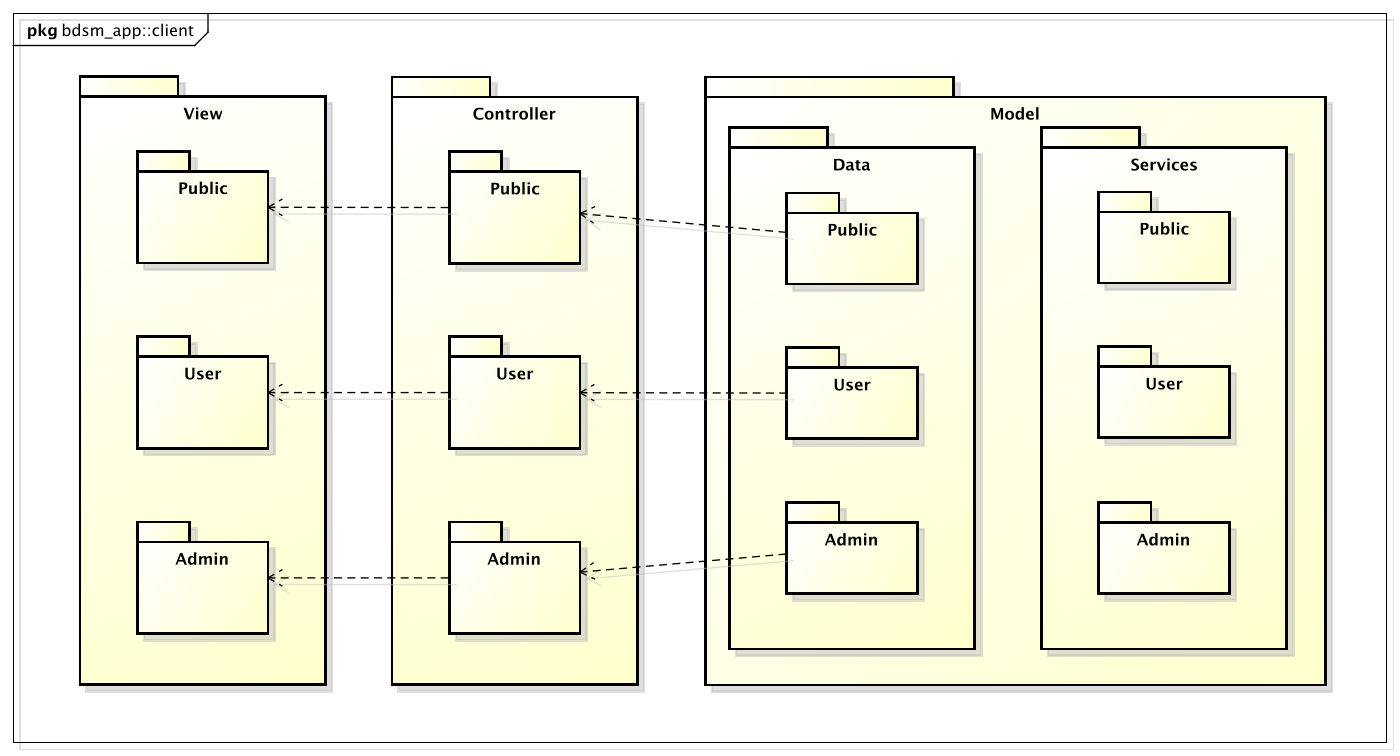
\includegraphics[scale=0.85]{./images/client/client.pdf}}
		\label{fig:package_client}
		\caption{Package - client}
	\end{figure}

	\begin{itemize}
		\item \textbf{Descrizione}: è il package che racchiude tutte le parti del front-end. \'E quindi l'insieme dei componenti che viene eseguito nel browser degli utenti normali e degli amministratori, fornendo loro un'interfaccia grafica per interagire con il sistema;
		\item \textbf{Package contenuti}:
			\begin{itemize}
				\item client::model
				\item client::view
				\item client::controller
			\end{itemize}
		\item \textbf{Interazione con altri componenti}: interagisce con il server definito nella sezione \ref{sub:server} effettuando delle chiamate ai servizi REST esposti;
	\end{itemize}
	% subsubsection bdsm_app_client (end)

	\pagebreak
	% PACKAGE MODEL
	% =================================================================================================
% File:			client_tier/model.tex
% Description:	Defiinisce la sezione relativa al front-end dell'applicazione
% Created:		2015-04-07
% Author:		Tesser Paolo
% Email:		tesser.paolo@mashup-unipd.it
% =================================================================================================
% Modification History:
% Version		Modifier Date		Change											Author
% 0.0.1 		2015-04-07 			creato scheletro								Tesser Paolo
% =================================================================================================
%
%

% CONTENUTO DEL CAPITOLO


\subsubsection{bdsm\_app::client::model} % (fold)
\label{ssub:bdsm_app_client_model}
[TO DO] (diagramma) \newline \newline

\begin{itemize}
	\item \textbf{Descrizione}: [TO DO];
	\item \textbf{Padre}: client;
	\item \textbf{Package contenuti}:
		\begin{itemize}
			\item client::model::data
			\item client::model::services
		\end{itemize}
	\item \textbf{Interazione con altri componenti}: [TO DO];
\end{itemize}
% subsubsection bdsm_app_client_model (end)


\subsubsection{bdsm\_app::client::model::data} % (fold)
\label{ssub:bdsm_app_client_model_data}
[TO DO] (diagramma) \newline \newline

\begin{itemize}
	\item \textbf{Descrizione}: [TO DO];
	\item \textbf{Padre}: client::model
	\item \textbf{Package contenuti}:
		\begin{itemize}
			\item client::model::data::public
			\item client::model::data::user
			\item client::model::data::admin
		\end{itemize}
	\item \textbf{Interazione con altri componenti}: [TO DO];
	
	\paragraph{Classi} % (fold)
		\subparagraph{Nome package::Nome classe} % (fold)
		\label{subp:subparagraph_name}
			\begin{itemize}
				\item \textbf{Descrizione}: [TO DO];
				\item \textbf{Utilizzo}: [TO DO];
				\item \textbf{Classi ereditate}: [TO DO];
				\item \textbf{Relazioni con altre classi}: [TO DO].
			\end{itemize}
\end{itemize}
% subsubsection bdsm_app_client_model_data (end)



\subsubsection{bdsm\_app::client::model::services} % (fold)
\label{ssub:bdsm_app_client_model_services}
[TO DO] (diagramma) \newline \newline

\begin{itemize}
	\item \textbf{Descrizione}: [TO DO];
	\item \textbf{Padre}: client::model
	\item \textbf{Package contenuti}:
		\begin{itemize}
			\item client::model::services::public
			\item client::model::services::user
			\item client::model::services::admin
		\end{itemize}
	\item \textbf{Interazione con altri componenti}: [TO DO];
	
	\paragraph{Classi} % (fold)
		\subparagraph{Nome package::Nome classe} % (fold)
		\label{subp:subparagraph_name}
			\begin{itemize}
				\item \textbf{Descrizione}: [TO DO];
				\item \textbf{Utilizzo}: [TO DO];
				\item \textbf{Classi ereditate}: [TO DO];
				\item \textbf{Relazioni con altre classi}: [TO DO].
			\end{itemize}

\end{itemize}
% subsubsection bdsm_app_client_model_services (end)
 \clearpage \newpage
	% END PACKAGE MODEL

	% PACKAGE DELLA VIEW
	% =================================================================================================
% File:			client_tier/view.tex
% Description:	Defiinisce la sezione relativa al front-end dell'applicazione
% Created:		2015-04-07
% Author:		Tesser Paolo
% Email:		tesser.paolo@mashup-unipd.it
% =================================================================================================
% Modification History:
% Version		Modifier Date		Change											Author
% 0.0.1 		2015-04-07 			creato scheletro								Tesser Paolo
% =================================================================================================
% 0.0.2			2015-04-07			descrizione delle classi						Carnovalini Filippo
% =================================================================================================
% 0.0.3			2015-04-08			aggiunte classi sulle relazioni					Tesser Paolo
% =================================================================================================
%

% CONTENUTO DEL CAPITOLO

\subsubsection{client::view} % (fold)
\label{ssub:bdsm_app_client_view}
In questa sezione e in tutte quelle inerenti al package \textbf{view}, il termine classe e pagina HTML, saranno sinonimi.
\begin{figure}[htbp]
	\centering
	\centerline{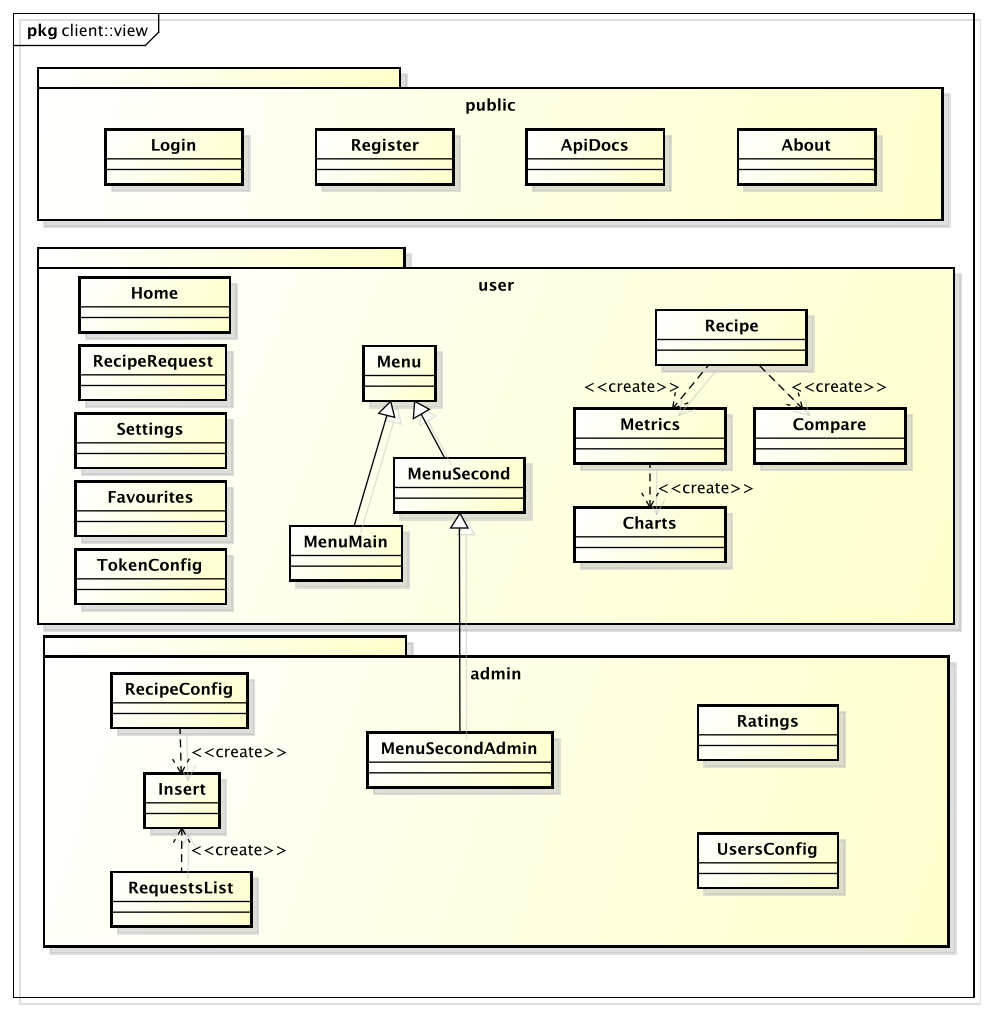
\includegraphics[scale=0.5]{./images/client/client_view.pdf}}
	\caption{Package - client::view}
\end{figure}

\begin{itemize}
	\item \textbf{Descrizione}: è il package che contiene tutte le classi che costituiscono la view del client. Ogni classe è equivalenti a un template di pagina HTML che sarà presentato all'utente, quando richiesto, tramite un sistema di routing. \newline
	All'interno di esso sono presenti altri componenti che separano le pagine HTML offerte, a seconda dei permessi che possiede un utente;
	\item \textbf{Padre}: client
	\item \textbf{Package contenuti}:
		\begin{itemize}
			\item client::view::public
			\item client::view::user
			\item client::view::admin
		\end{itemize}
	\item \textbf{Interazione con altri componenti}:
		\begin{itemize}
			\item client::controller
		\end{itemize}
\end{itemize}
% subsubsection bdsm_app_client_view (end)

\pagebreak

\subsubsection{client::view::public} % (fold)
\label{ssub:bdsm_app_client_view_public}
\begin{figure}[htbp]
	\centering
	\centerline{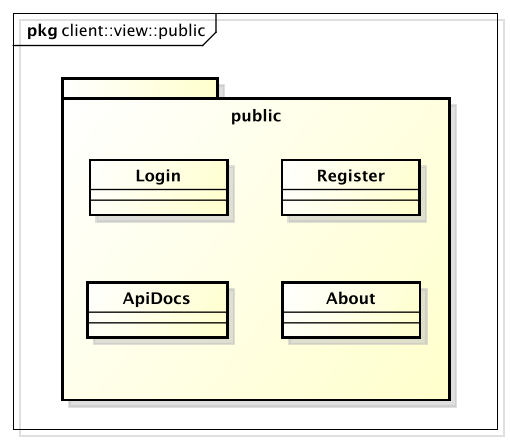
\includegraphics[scale=0.6]{./images/client/client_view_public.pdf}}
	\caption{Package - client::view::public}
\end{figure}

\begin{itemize}
	\item \textbf{Descrizione}: è il package che contiene tutte le pagine HTML che possono essere offerte quando l'utente deve ancora effettuare l'accesso al sistema;
	\item \textbf{Padre}: client::view
	\item \textbf{Interazione con altri componenti}:
		\begin{itemize}
			\item client::controller::public
		\end{itemize}
\end{itemize}

	\paragraph{Classi} % (fold)
		\subparagraph{client::view::public::Login} % (fold)
		\label{subp:bdsm_app_client_view_public_login}

			\begin{itemize}
				\item \textbf{Descrizione}: la classe rappresenta un template HTML per la visualizzazione dell'interfaccia di autenticazione;
				\item \textbf{Utilizzo}: viene utilizzata per generare la pagina HTML di autenticazione;
				\item \textbf{Relazioni con altre classi}:
					\begin{itemize}
						\item client::controller::public::PublicRoute
						\item client::controller::public::LoginCtrl
					\end{itemize}
				\item \textbf{Direttive AngularJS}:
					\begin{itemize}
						\item \textbf{ng-controller}: permette l'attivazione del controller associato al template HTML relativo alla pagina di Login;
						\item \textbf{ng-submit}: rileva una scelta di invio dati dell'utente e attiva una funzione, in questo caso \textbf{login(credentials)} definita in LoginCtrl;
						\item \textbf{ng-model}: permette di creare un legame tra le variabili presenti nel controller e i campi di tipo input dell'HTML, realizzando così il two-way data binding.
						\item \textbf{ng-disabled}: permette di bloccare un determinato campo fintanto che una o più condizioni non vengono soddisfatte. Viene utilizzata per bloccare il pulsante di login qualora non fossero stati completati correttamente i campi presenti.
					\end{itemize}
			\end{itemize}
		% subparagraph bdsm_app_client_view_public_login (end)

		\subparagraph{client::view::public::About} % (fold)
		\label{subp:bdsm_app_client_view_public_about}
			\begin{itemize}
				\item \textbf{Descrizione}: la classe rappresenta un template HTML per la visualizzazione della pagina di informazioni sull'applicazione;
				\item \textbf{Utilizzo}: viene usata per generare la pagina HTML di About;
				\item \textbf{Relazioni con altre classi}:
					\begin{itemize}
						\item client::controller::public::PublicRoute
					\end{itemize}
				\item \textbf{Direttive AngularJS}: non sono state utilizzate direttive in quanto è una pagina statica senza bisogno di interazioni con l'utente.
			\end{itemize}
		% subparagraph bdsm_app_client_view_public_about (end)

		\subparagraph{client::view::public::Register} % (fold)
		\label{subp:bdsm_app_client_view_public_register}
			\begin{itemize}
				\item \textbf{Descrizione}: la classe rappresenta un template HTML per la visualizzazione dell'interfaccia di registrazione al servizio;
				\item \textbf{Utilizzo}: viene utilizzata per generare la pagina HTML di registrazione;
				\item \textbf{Relazioni con altre classi}:
					\begin{itemize}
						\item client::controller::public::PublicRoute
						\item client::controller::public::RegisterCtrl
					\end{itemize}
				\item \textbf{Direttive AngularJS}:
					\begin{itemize}
						\item \textbf{ng-controller}: permette l'attivazione del controller associato al template HTML relativo alla pagina di registrazione;
						\item \textbf{ng-submit}: rileva una scelta di invio dati dell'utente e attiva una funzione, in questo caso \textbf{register(credentials)} definita in RegisterCtrl;
						\item \textbf{ng-disabled}: permette di bloccare un determinato campo fintanto che una o più condizioni non vengono soddisfatte. Viene utilizzata per bloccare il pulsante di login qualora non fossero stati completati correttamente i campi presenti;
						\item \textbf{ng-model}: permette di creare un legame tra le variabili presenti nel controller e i campi di tipo input dell'HTML, realizzando così il two-way data binding;
						\item \textbf{ng-message}: permette di visualizzare un determinato messaggio che viene associato ad un particolare errore scaturito nel form di registrazione;
						\item \textbf{ng-if}: permette di visualizzare un determinato elemento, e il contenuto al suo interno, qualora la condizione specificata risultasse vera. Viene utilizzata per nascondere i messaggi d'errore e renderli visibili qualora l'errore si verificasse;
						\item \textbf{ng-class}: permette di associare una determinata classe, a un elemento del template, qualora la condizione specificata risultasse vera. Questa viene utilizzata per mostrare un colore rosso d'errore sui campi che non soddisfano le specifiche richieste dal form.
					\end{itemize}
			\end{itemize}
		% subparagraph bdsm_app_client_view_public_register (end)

		\subparagraph{client::view::public::ApiDocs} % (fold)
		\label{subp:bdsm_app_client_view_public_apidocs}
		
			\begin{itemize}
				\item \textbf{Descrizione}: la classe rappresenta un template HTML per la visualizzazione della pagina contenente la documentazione dei servizi REST offerti;
				\item \textbf{Utilizzo}: viene utilizzata per generare la pagina HTML contenente la documentazione dei servizi offerti;
				\item \textbf{Relazioni con altre classi}:
					\begin{itemize}
						\item client::controller::public::PublicRoute
						\item client::controller::public::ApiDocsCtrl
					\end{itemize}
				\item \textbf{Direttive AngularJS}:
					\begin{itemize}
						\item \textbf{ng-controller}: permette l'attivazione del controller associato al template HTML relativo alla pagina di visualizzazione delle API disponibili a un utente che ha ottenuto un token di accesso per usarle;
						\item \textbf{ng-repeat}: permette di iterare ogni elemento di una lista e di poterlo utilizzare all'interno del template HTML grazie alla direttiva \textbf{ng-bind} potendone ricavare dati o eseguire metodi su di esso. Viene utilizzata per stampare la lista di tutte le API e la loro descrizione;
						\item \textbf{ng-bind}: permette di rimpiazzare il contenuto di un elemento con il valore dato dall'espressione definita. Questa direttiva viene preferita all'uso dell'operatore \{\{ \}\}. Viene utilizzata per stampare il valore degli elementi che si stanno iterando tramite la direttiva \textbf{ng-repeat}.
					\end{itemize}
			\end{itemize}
		% subparagraph bdsm_app_client_view_public_apidocs (end)

% subsubsection bdsm_app_client_view_public (end)


\subsubsection{client::view::user} % (fold)
\label{ssub:bdsm_app_client_view_user}
\begin{figure}[htbp]
	\centering
	\centerline{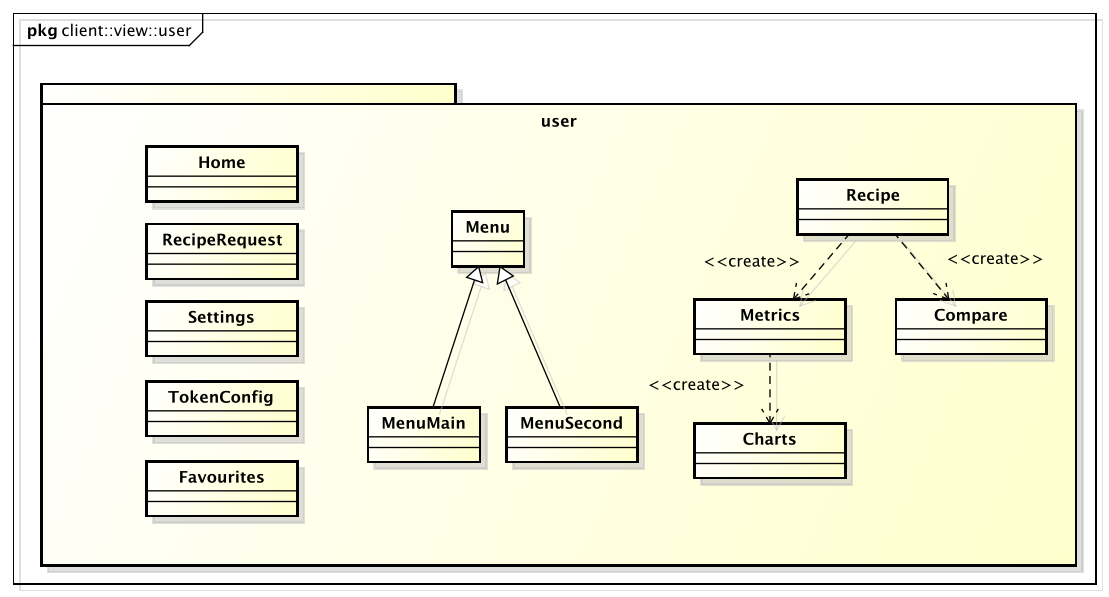
\includegraphics[scale=0.95]{./images/client/client_view_user.pdf}}
	\caption{Package - client::view::user}
\end{figure}

\begin{itemize}
	\item \textbf{Descrizione}: è il package che contiene tutte le pagine HTML che ha a disposizione l'utente che ha effettuato l'accesso al sistema, sia che sia un utente normale sia che sia un amministratore. \newline
	Per semplicità e chiarezza non è stato evidenziato nel grafico il fatto che ogni classe di questo package possiede un'istanza di MenuMain e di MenuSecond.
	\item \textbf{Padre}: client::view
	\item \textbf{Interazione con altri componenti}:
		\begin{itemize}
			\item client::controller::user
		\end{itemize}
\end{itemize}

	\paragraph{Classi} % (fold)
		\subparagraph{client::view::user::Home} % (fold)
		\label{subp:bdsm_app_client_view_user_home}

			\begin{itemize}
				\item \textbf{Descrizione}: la classe rappresenta un template HTML contenente lo scheletro delle pagine destinate a uno User e a un Admin;
				\item \textbf{Utilizzo}: viene utilizzata per generare lo scheletro della pagina HTML utilizzata come base da altre pagine;
				\item \textbf{Relazioni con altre classi}:
					\begin{itemize}
						\item client::view::user::MenuMain
						\item client::view::user::MenuSecond
						\item client::controller::public::HomeRoute
					\end{itemize}
				\item \textbf{Direttive AngularJS}:
					\begin{itemize}
						\item \textbf{ui-view}: direttiva utilizzata dal modulo \textbf{ui-router} che permette il caricamento del template HTML corretto a secondo di un determinato url o di uno stato attivato tramite la direttiva \textbf{ui-sref}.
					\end{itemize}
			\end{itemize}
		% subparagraph bdsm_app_client_view_user_home (end)

		\subparagraph{client::view::user::Recipe} % (fold)
		\label{subp:bdsm_app_client_view_user_recipe}

			\begin{itemize}
				\item \textbf{Descrizione}: la classe rappresenta un template HTML per la visualizzazione della pagina di visione delle recipe a disposizione;
				\item \textbf{Utilizzo}: viene usata per generare la pagina HTML di visione delle recipe;
				\item \textbf{Relazioni con altre classi}:
					\begin{itemize}
						\item client::view::user::MenuMain
						\item client::view::user::MenuSecond
						\item client::view::user::Metrics
						\item client::view::user::Compare
						\item client::controller::user::RecipeRoute
						\item client::controller::user::RecipeCtrl
					\end{itemize}
				\item \textbf{Direttive AngularJS}:
					\begin{itemize}
						\item \textbf{ng-controller}: permette l'attivazione del controller associato al template HTML relativo alla pagina di visualizzazione delle recipe presenti nel sistema;
						\item \textbf{ng-repeat}: permette di iterare ogni elemento di una lista e di poterlo utilizzare all'interno del template HTML grazie alla direttiva \textbf{ng-bind} potendone ricavare dati o eseguire metodi su di esso. Viene utilizzata per stampare la lista di tutte le recipe;
						\item \textbf{ng-bind}: permette di rimpiazzare il contenuto di un elemento con il valore dato dall'espressione definita. Questa direttiva viene preferita all'uso dell'operatore \{\{ \}\}. Viene utilizzata per stampare il valore degli elementi che si stanno iterando tramite la direttiva \textbf{ng-repeat}.
						\item \textbf{ui-sref}: permette di effettuare un reindirizzamento in una determinata pagina, con la possibilità di passare dei parametri. Viene utilizzata dai pulsanti \textbf{Show metrics} e \textbf{Compare metrics} per andare alle pagine Metrics e Compare a seconda delle necessità dell'utente.
					\end{itemize}
			\end{itemize}
		% subparagraph bdsm_app_client_view_user_recipe (end)

		\subparagraph{client::view::user::Metrics} % (fold)
		\label{subp:bdsm_app_client_view_metrics}

			\begin{itemize}
				\item \textbf{Descrizione}: la classe rappresenta un template HTML per la visualizzazione della pagina di visione delle metriche a disposizione per una selezionata recipe;
				\item \textbf{Utilizzo}: viene utilizzata per generare la pagina HTML di visione delle metriche quando viene selezionata una Recipe;
				\item \textbf{Relazioni con altre classi}:
					\begin{itemize}
						\item client::view::user::MenuMain
						\item client::view::user::MenuSecond
						\item client::view::user::Recipe
						\item client::view::user::Charts
						\item client::controller::user::RecipeRoute
						\item client::controller::user::MetricsCtrl
					\end{itemize}
				\item \textbf{Direttive AngularJS}:
					\begin{itemize}
						\item \textbf{ng-controller}: permette l'attivazione del controller associato al template HTML relativo alla pagina di visualizzazione delle metriche di una determinata recipe;
						\item \textbf{ng-repeat}: permette di iterare ogni elemento di una lista e di poterlo utilizzare all'interno del template HTML grazie alla direttiva \textbf{ng-bind} potendone ricavare dati o eseguire metodi su di esso. Viene utilizzata per stampare la lista di tutte le metriche relative a una determinata recipe;
						\item \textbf{ng-bind}: permette di rimpiazzare il contenuto di un elemento con il valore dato dall'espressione definita. Questa direttiva viene preferita all'uso dell'operatore \{\{ \}\}. Viene utilizzata per stampare il valore degli elementi che si stanno iterando tramite la direttiva \textbf{ng-repeat}.
						\item \textbf{ui-sref}: permette di effettuare un reindirizzamento in una determinata pagina, con la possibilità di passare dei parametri. Viene utilizzata dai pulsanti \textbf{Show charts} per andare alla pagina che visualizza tutti i grafici associati a una determinata metrica. 
					\end{itemize}
			\end{itemize}
		% subparagraph bdsm_app_client_view_metrics (end)

		\subparagraph{client::view::user::Charts} % (fold)
		\label{subp:bdsm_app_client_view_user_charts}

			\begin{itemize}
				\item \textbf{Descrizione}: la classe rappresenta un template HTML per la visualizzazione della pagina di visione delle view associate ad una metrica selezionata;
				\item \textbf{Utilizzo}: viene usata per generare la pagina HTML di visione delle view quando viene selezionata una metrica;
				\item \textbf{Relazioni con altre classi}:
					\begin{itemize}
						\item client::view::user::MenuMain
						\item client::view::user::MenuSecond
						\item client::view::user::Metrics
						\item client::controller::user::RecipeRoute
						\item client::controller::user::ChartsCtrl
					\end{itemize}
				\item \textbf{Direttive AngularJS}:
						\item \textbf{ng-controller}: permette l'attivazione del controller associato al template HTML relativo alla pagina di visualizzazione di grafici generati da una metrica o da confronto;
						\item \textbf{ng-repeat}: permette di iterare ogni elemento di una lista e di poterlo utilizzare all'interno del template HTML grazie alla direttiva \textbf{ng-bind} potendone ricavare dati o eseguire metodi su di esso. Viene utilizzata per visualizzare tutti i grafici generati;
						\item \textbf{ng-bind}: permette di rimpiazzare il contenuto di un elemento con il valore dato dall'espressione definita. Questa direttiva viene preferita all'uso dell'operatore \{\{ \}\}. Viene utilizzata per stampare la descrizione dei grafici che si stanno iterando tramite la direttiva \textbf{ng-repeat}.
						\item \textbf{ng-bind-html}: permette di rimpiazzare il contenuto di un elemento con del codice HTML che non viene interpretato come stringa ma come codice della pagina. Viene usato per 
						il valore dato dall'espressione definita. Questa direttiva viene preferita all'uso dell'operatore \{\{ \}\}. Viene utilizzata per visualizzare i grafici che si stanno iterando tramite la direttiva \textbf{ng-repeat}.
			\end{itemize}
		% subparagraph bdsm_app_client_view_user_charts (end)

		\subparagraph{client::view::user::Compare} % (fold)
		\label{subp:bdsm_app_client_view_user_compare}

			\begin{itemize}
				\item \textbf{Descrizione}: la classe rappresenta un template HTML per la visualizzazione dell'interfaccia di confronto tra diverse metriche di una recipe;
				\item \textbf{Utilizzo}: viene utilizzata per generare la pagina HTML di confronto tra metriche;
				\item \textbf{Relazioni con altre classi}:
					\begin{itemize}
						\item client::view::user::MenuMain
						\item client::view::user::MenuSecond
						\item client::view::user::Recipe
						\item client::controller::user::RecipeRoute
						\item client::controller::user::CompareCtrl
					\end{itemize}
				\item \textbf{Direttive AngularJS}:
					\begin{itemize}
						\item \textbf{ng-controller}: permette l'attivazione del controller associato al template HTML relativo alla pagina di che permette di confronta più metriche di una stessa Recipe;
						\item \textbf{ng-submit}: permette di rilevare una scelta di invio dati dell'utente e attiva una funzione, in questo caso \textbf{generate()} definita in CompareCtrl;
						\item \textbf{ng-click}: permette di rilevare una scelta dell'utente e attiva una funzione, in questo caso \textbf{addMetric()} definita in CompareCtrl;
						\item \textbf{ng-change}: permette di rilevare un cambiamento su un determinato elemento di una form, in questo caso aggiorna i valori di alcuni array a seconda del tipo di cambiamento che viene effettuato;
						\item \textbf{ng-if}: permette di visualizzare un determinato elemento, e il contenuto al suo interno, qualora la condizione specificata risultasse vera. Viene utilizzata per nascondere i messaggi d'errore e renderli visibili qualora l'errore si verificasse;
						\item \textbf{ng-repeat}: permette di iterare ogni elemento di una lista e di poterlo utilizzare all'interno del template HTML grazie alla direttiva \textbf{ng-bind} potendone ricavare dati o eseguire metodi su di esso. Viene utilizzata per stampare la lista di tutte le metriche aggiunte alla richiesta di confronto;
						\item \textbf{ng-bind}: permette di rimpiazzare il contenuto di un elemento con il valore dato dall'espressione definita. Questa direttiva viene preferita all'uso dell'operatore \{\{ \}\}. Viene utilizzata per stampare il valore degli elementi che si stanno iterando tramite la direttiva \textbf{ng-repeat}.
					\end{itemize}
			\end{itemize}
		% subparagraph bdsm_app_client_view_user_compare (end)

		\subparagraph{client::view::user::RecipeRequest} % (fold)
		\label{subp:bdsm_app_client_view_user_reciperequest}
			\begin{itemize}
				\item \textbf{Descrizione}: la classe rappresenta un template HTML per la visualizzazione dell'interfaccia di richiesta di una nuova recipe;
				\item \textbf{Utilizzo}: viene utilizzata per generare la pagina HTML di richiesta di una nuova recipe;
				\item \textbf{Relazioni con altre classi}:
					\begin{itemize}
						\item client::view::user::MenuMain
						\item client::view::user::MenuSecond
						\item client::controller::user::RecipeRequestRoute
						\item client::controller::user::RecipeRequestCtrl
					\end{itemize}
				\item \textbf{Direttive AngularJS}:
					\begin{itemize}
						\item \textbf{ng-controller}: permette l'attivazione del controller associato al template HTML relativo alla pagina di visualizzazione del form di richiesta di inserimento di una nuova recipe;
						\item \textbf{ng-submit}: permette di rilevare una scelta di invio dati dell'utente e attiva una funzione, in questo caso \textbf{insertRecipeRequest()} definita in RecipeRequestCtrl;
						\item \textbf{ng-click}: permette di rilevare una scelta dell'utente e attiva una funzione, in questo caso \textbf{addMetric()} definita in RecipeRequestCtrl.
						\item \textbf{ng-disabled}: permette di bloccare un determinato campo fintanto che una o più condizioni non vengono soddisfatte. Viene utilizzata per bloccare il pulsante di inserimento della richiesta qualora non fossero stati completati correttamente i campi presenti;
						\item \textbf{ng-model}: permette di creare un legame tra le variabili presenti nel controller e i campi di tipo input dell'HTML, realizzando così il two-way data binding;
						\item \textbf{ng-if}: permette di visualizzare un determinato elemento, e il contenuto al suo interno, qualora la condizione specificata risultasse vera. Viene utilizzata per nascondere i messaggi d'errore e renderli visibili qualora l'errore si verificasse;
						\item \textbf{ng-repeat}: permette di iterare ogni elemento di una lista e di poterlo utilizzare all'interno del template HTML grazie alla direttiva \textbf{ng-bind} potendone ricavare dati o eseguire metodi su di esso. Viene utilizzata per stampare la lista di tutte le metriche aggiunte alla richiesta di inserimento di una recipe;
						\item \textbf{ng-bind}: permette di rimpiazzare il contenuto di un elemento con il valore dato dall'espressione definita. Questa direttiva viene preferita all'uso dell'operatore \{\{ \}\}. Viene utilizzata per stampare il valore degli elementi che si stanno iterando tramite la direttiva \textbf{ng-repeat}.
					\end{itemize}
			\end{itemize}
		% subparagraph bdsm_app_client_view_user_reciperequest (end)

		\subparagraph{client::view::user::Favourites} % (fold)
		\label{subp:bdsm_app_client_view_user_favourites}

			\begin{itemize}
				\item \textbf{Descrizione}: la classe rappresenta un template HTML per la visualizzazione della pagina contenente le view preferite;
				\item \textbf{Utilizzo}: viene utilizzata per generare la pagina HTML delle view preferite;
				\item \textbf{Relazioni con altre classi}:
					\begin{itemize}
						\item client::view::user::MenuMain
						\item client::view::user::MenuSecond
						\item client::controller::user::FavouritesRoute
						\item client::controller::user::FavouritesCtrl
					\end{itemize}
				\item \textbf{Direttive AngularJS}:
					\begin{itemize}
						\item \textbf{ng-controller}: permette l'attivazione del controller associato al template HTML relativo alla pagina di visualizzazione dei grafici preferiti;
						\item \textbf{ng-repeat}: permette di iterare ogni elemento di una lista e di poterlo utilizzare all'interno del template HTML grazie alla direttiva \textbf{ng-bind} potendone ricavare dati o eseguire metodi su di esso. Viene utilizzata per visualizzare tutti i grafici favoriti;
						\item \textbf{ng-bind}: permette di rimpiazzare il contenuto di un elemento con il valore dato dall'espressione definita. Questa direttiva viene preferita all'uso dell'operatore \{\{ \}\}. Viene utilizzata per stampare la descrizione dei grafici che si stanno iterando tramite la direttiva \textbf{ng-repeat}.
						\item \textbf{ng-bind-html}: permette di rimpiazzare il contenuto di un elemento con del codice HTML che non viene interpretato come stringa ma come codice della pagina. Viene usato per 
						il valore dato dall'espressione definita. Questa direttiva viene preferita all'uso dell'operatore \{\{ \}\}. Viene utilizzata per visualizzare i grafici che si stanno iterando tramite la direttiva \textbf{ng-repeat}.
					\end{itemize}
			\end{itemize}
		% subparagraph bdsm_app_client_view_user_favourites (end)

		\subparagraph{client::view::user::TokenConfig} % (fold)
		\label{subp:bdsm_app_client_view_user_tokenconfig}

			\begin{itemize}
				\item \textbf{Descrizione}: la classe rappresenta un template HTML per la visualizzazione dell'interfaccia di gestione dei token per l'utilizzo dei servizi REST;
				\item \textbf{Utilizzo}: viene utilizzata per generare la pagina HTML di gestione dei token per i servizi REST;
				\item \textbf{Relazioni con altre classi}:
					\begin{itemize}
						\item client::view::user::MenuMain
						\item client::view::user::MenuSecond
						\item client::controller::user::TokenConfigRoute
						\item client::controller::user::TokenConfigCtrl
					\end{itemize}
				\item \textbf{Direttive AngularJS}:
					\begin{itemize}
						\item \textbf{ng-controller}: permette l'attivazione del controller associato al template HTML relativo alla pagina di visualizzazione del form di richiesta/cancellazione di un token di accesso ai servizi REST;
						\item \textbf{ng-if}: permette di visualizzare un determinato elemento, e il contenuto al suo interno, qualora la condizione specificata risultasse vera. Viene utilizzata per alternare i pulsanti di richiesta/cancellazione del token di accesso, a seconda se esso sia già stato generato o meno;
						\item \textbf{ng-bind}: permette di rimpiazzare il contenuto di un elemento con il valore dato dall'espressione definita. Questa direttiva viene preferita all'uso dell'operatore \{\{ \}\}. Viene utilizzata per stampare il valore del token generato.
					\end{itemize}
			\end{itemize}
		% subparagraph bdsm_app_client_view_user_tokenconfig (end)

		\subparagraph{client::view::user::Settings} % (fold)
		\label{subp:bdsm_app_client_view_user_settings}

			\begin{itemize}
				\item \textbf{Descrizione}: la classe rappresenta un template HTML per la visualizzazione dell'interfaccia di gestione delle opzioni;
				\item \textbf{Utilizzo}: viene utilizzata per generare la pagina HTML delle opzioni;
				\item \textbf{Relazioni con altre classi}:
					\begin{itemize}
						\item client::view::user::MenuMain
						\item client::view::user::MenuSecond
						\item client::controller::user::SettingsRoute
						\item client::controller::user::SettingsCtrl
					\end{itemize}
				\item \textbf{Direttive AngularJS}:
					\begin{itemize}
						\item \textbf{ng-controller}: permette l'attivazione del controller associato al template HTML relativo alla pagina di visualizzazione del form delle impostazioni personali del profilo utente;
						\item \textbf{ng-init}: permette di inizializzare una variabile definita all'interno del template con un determinato valore. Viene utilizzata per impostare le variabili \textbf{editUserName} e \textbf{editMail} inizialmente a \textbf{true};
						\item \textbf{ng-model}: permette di creare un legame tra le variabili presenti nel controller e i campi di tipo input dell'HTML, realizzando così il two-way data binding;
						\item \textbf{ng-submit}: permette di rilevare una scelta di invio dati dell'utente e attiva una funzione, in questo caso \textbf{saveEdit()} definita in SettingsCtrl;
						\item \textbf{ng-click}: permette di rilevare una scelta dell'utente e attiva una funzione o cambia il valore di qualche variabile dichiarata all'interno del template, in questo caso cambia la variabile \textbf{editUserName} o \textbf{editMail} nel valore \textbf{editUserName} o \textbf{editMail};
						\item \textbf{ng-disabled}: permette di bloccare un determinato campo fintanto che una o più condizioni non vengono soddisfatte. Viene utilizzata per bloccare il pulsante di salvataggio delle modifiche o per bloccare i campi di modifica della password e della mail, attivabile solo premendo su un apposito pulsante.
					\end{itemize}
			\end{itemize}
		% subparagraph bdsm_app_client_view_user_settings (end)

		\subparagraph{client::view::user::Menu} % (fold)
		\label{subp:bdsm_app_client_view_user_menu}
			\begin{itemize}
				\item \textbf{Descrizione}: questa classe astratta rappresenta un template HTML per la creazione di un menù;
				\item \textbf{Utilizzo}: non viene mai istanziata nel sistema, viene ereditata dalla classi che istanziano dei menù;
				\item \textbf{Relazioni con altre classi}:
					\begin{itemize}
						\item client::view::user::MenuMain
						\item client::view::user::MenuSecond
						\item client::controller::user::MenuCtrl
					\end{itemize}
			\end{itemize}
		% subparagraph bdsm_app_client_view_user_menu (end)

		\subparagraph{client::view::user::MenuMain} % (fold)
		\label{subp:bdsm_app_client_view_user_menumain}

			\begin{itemize}
				\item \textbf{Descrizione}: la classe rappresenta un template HTML per la creazione del menù principale;
				\item \textbf{Utilizzo}: viene usata nel generare ogni pagina usata da un utente autenticato per generare il menù principale in essa contenuta;
				\item \textbf{Classi ereditate}:
					\begin{itemize}
						\item client::view::user::Menu
					\end{itemize}
				\item \textbf{Relazioni con altre classi}:
					\begin{itemize}
						\item client::view::user::Menu
						\item client::controller::user::MenuMainCtrl
					\end{itemize}
				\item \textbf{Direttive AngularJS}:
					\begin{itemize}
						\item \textbf{ui-sref}: permette di effettuare un reindirizzamento in una determinata pagina, con la possibilità di passare dei parametri. Viene utilizzata dai pulsanti presenti nel menu principale per navigare in alcune delle pagine del sistema;
					\end{itemize}
			\end{itemize}
		% subparagraph bdsm_app_client_view_user_menumain (end)

		\subparagraph{client::view::user::MenuSecond} % (fold)
		\label{subp:bdsm_app_client_view_user_menusecond}

			\begin{itemize}
				\item \textbf{Descrizione}: la classe rappresenta un template HTML per la creazione del menù secondario di un utente non amministratore;
				\item \textbf{Utilizzo}: viene usata nel generare ogni pagina di un utente autenticato non amministratore per generare il menù secondario;
				\item \textbf{Classi ereditate}:
					\begin{itemize}
						\item client::view::user::Menu
					\end{itemize}
				\item \textbf{Relazioni con altre classi}:
					\begin{itemize}
						\item client::view::user::Menu
						\item client::view::admin::MenuSecondAdmin
						\item client::controller::user::MenuSecondCtrl
					\end{itemize}
				\item \textbf{Direttive AngularJS}:
					\begin{itemize}
						\item \textbf{ui-sref}: permette di effettuare un reindirizzamento in una determinata pagina, con la possibilità di passare dei parametri. Viene utilizzata dai pulsanti presenti nel menu secondario per navigare in alcune delle pagine del sistema;
					\end{itemize}
			\end{itemize}
		% subparagraph bdsm_app_client_view_user_menusecond (end)
% subsubsection bdsm_appclient__view_user (end)

\subsubsection{client::view::admin} % (fold)
\label{ssub:bdsm_app_client_view_admin}
\begin{figure}[htbp]
	\centering
	\centerline{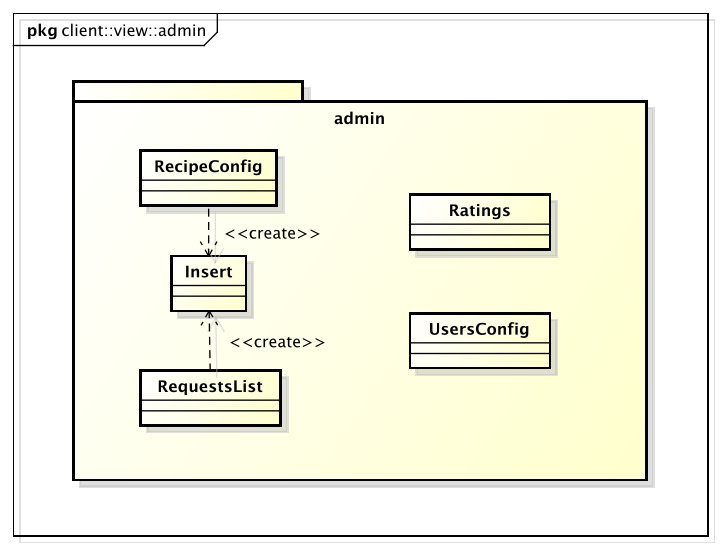
\includegraphics[scale=0.49]{./images/client/client_view_admin.pdf}}
	\caption{Package - client::view::admin}
\end{figure}

\begin{itemize}
	\item \textbf{Descrizione}: è il package che contiene tutte le pagine HTML che ha a disposizione l'utente che ha i privilegi di amministratore;\newline
	Per semplicità e chiarezza non è stato evidenziato nel grafico il fatto che ogni classe di questo package possiede un'istanza di MenuMain e di MenuSecondAdmin.
	\item \textbf{Padre}: client::view
	\item \textbf{Interazione con altri componenti}:
		\begin{itemize}
			\item client::controller::admin
		\end{itemize}
\end{itemize}

	\paragraph{Classi} % (fold)
		\subparagraph{client::view::admin::RecipeConfig} % (fold)
		\label{subp:bdsm_app_client_view_admin_recipeconfig}

			\begin{itemize}
				\item \textbf{Descrizione}: la classe rappresenta un template HTML per la visualizzazione dell'interfaccia di gestione delle Recipe;
				\item \textbf{Utilizzo}: viene utilizzata per generare la pagina HTML della gestione delle Recipe;
				\item \textbf{Relazioni con altre classi}:
					\begin{itemize}
						\item client::view::user::MenuMain
						\item client::view::admin::MenuSecondAdmin
						\item client::view::admin::Insert
						\item client::controller::admin::RecipeConfigRoute
						\item client::controller::admin::RecipeConfigCtrl
					\end{itemize}
				\item \textbf{Direttive AngularJS}:
					\begin{itemize}
						\item \textbf{ng-controller}: permette l'attivazione del controller associato al template HTML relativo alla pagina di inserimento di nuove recipe;
					\end{itemize}
			\end{itemize}
		% subparagraph bdsm_app_client_view_admin_recipeconfig (end)

		\subparagraph{client::view::admin::RequestList} % (fold)
		\label{subp:bdsm_app_client_view_admin_requestlist}

			\begin{itemize}
				\item \textbf{Descrizione}: la classe rappresenta un template HTML per la visualizzazione della pagina di visione delle richieste di Recipe;
				\item \textbf{Utilizzo}: viene utilizzata per generare la pagina HTML della lista delle richieste di Recipe;
				\item \textbf{Relazioni con altre classi}:
					\begin{itemize}
						\item client::view::user::MenuMain
						\item client::view::admin::MenuSecondAdmin
						\item client::view::admin::Insert
						\item client::controller::admin::RequestListRoute
						\item client::controller::admin::RequestListCtrl
					\end{itemize}
				\item \textbf{Direttive AngularJS}:
					\begin{itemize}
						\item \textbf{ng-controller}: permette l'attivazione del controller associato al template HTML relativo alla pagina di visualizzazione delle richieste di nuove recipe;
						\item \textbf{ng-click}: permette di rilevare una scelta dell'utente e attiva una funzione o cambia il valore di qualche variabile dichiarata all'interno del template, in questo viene utilizzato da due pulsanti che attivano le relative funzioni \textbf{discardRequest(idRequestRecipe)} e \textbf{approvedRequest(idRequestRecipe)};
						\item \textbf{ng-repeat}: permette di iterare ogni elemento di una lista e di poterlo utilizzare all'interno del template HTML grazie alla direttiva \textbf{ng-bind} potendone ricavare dati o eseguire metodi su di esso. Viene utilizzata per stampare la lista di tutte le richieste di nuove recipe;
						\item \textbf{ng-bind}: permette di rimpiazzare il contenuto di un elemento con il valore dato dall'espressione definita. Questa direttiva viene preferita all'uso dell'operatore \{\{ \}\}. Viene utilizzata per stampare il valore degli elementi che si stanno iterando tramite la direttiva \textbf{ng-repeat};
						\item \textbf{ui-sref}: permette di effettuare un reindirizzamento in una determinata pagina, con la possibilità di passare dei parametri. Viene utilizzata dal pulsante \textbf{See Details} che manda alla visualizzazione dei dettagli di una richiesta particolare.
					\end{itemize}
			\end{itemize}
		% subparagraph bdsm_app_client_view_admin_requestlist (end)

		\subparagraph{client::view::admin::Insert} % (fold)
		\label{subp:bdsm_app_client_view_admin_insert}

			\begin{itemize}
				\item \textbf{Descrizione}: la classe rappresenta un template HTML per la visualizzazione dell'interfaccia di inserimento di una nuova Recipe;
				\item \textbf{Utilizzo}: viene utilizzata per generare la pagina HTML di inserimento di una nuova recipe;
				\item \textbf{Relazioni con altre classi}:
					\begin{itemize}
						\item client::view::user::MenuMain
						\item client::view::admin::MenuSecondAdmin
						\item client::view::admin::RecipeConfig
						\item client::view::admin::RequestList
						\item client::controller::admin::RecipeConfigRoute
						\item client::controller::admin::InsertRecipeCtrl
					\end{itemize}
				\item \textbf{Direttive AngularJS}:
					\begin{itemize}
						\item \textbf{ng-controller}: permette l'attivazione del controller associato al template HTML relativo al form di inserimento di nuova recipe;
						\item \textbf{ng-submit}: rileva una scelta di invio dati dell'utente e attiva una funzione, in questo caso \textbf{insertRecipe()} definita in RecipeCtrl;
						\item \textbf{ng-click}: permette di rilevare una scelta dell'utente e attiva una funzione o cambia il valore di qualche variabile dichiarata all'interno del template, in questo viene utilizzato dal pulsante che aggiunge un metrica tramite la funzione \textbf{addMetric(cat, typeCat, value)};
						\item \textbf{ng-show}: permette di visualizzare o meno del contenuti HTML a seconda se una determina condizione sia verificata. Viene utilizzato per nascondere/visualizzare gli errori di inserimento dei campi dati o qualche informazione di successo delle operazioni previste;
						\item \textbf{ng-model}: permette di creare un legame tra le variabili presenti nel controller e i campi di tipo input dell'HTML, realizzando così il two-way data binding;
						\item \textbf{ng-repeat}: permette di iterare ogni elemento di una lista e di poterlo utilizzare all'interno del template HTML grazie alla direttiva \textbf{ng-bind} potendone ricavare dati o eseguire metodi su di esso. Viene utilizzata per stampare la lista di tutte le metriche che si vogliono aggiungere alla Recipe;
						\item \textbf{ng-bind}: permette di rimpiazzare il contenuto di un elemento con il valore dato dall'espressione definita. Questa direttiva viene preferita all'uso dell'operatore \{\{ \}\}. Viene utilizzata per stampare il valore degli elementi che si stanno iterando tramite la direttiva \textbf{ng-repeat};
					\end{itemize}
			\end{itemize}
		% subparagraph bdsm_app_client_view_admin_insert (end)

		\subparagraph{client::view::admin::Ratings} % (fold)
		\label{subp:bdsm_app_client_view_admin_ratings}

			\begin{itemize}
				\item \textbf{Descrizione}: la classe rappresenta un template HTML per la visualizzazione della pagina dei voti assegnati alle varie Recipe;
				\item \textbf{Utilizzo}: viene utilizzata per generare la pagina HTML di visione dei voti delle Recipe;
				\item \textbf{Relazioni con altre classi}:
					\begin{itemize}
						\item client::view::user::MenuMain
						\item client::view::admin::MenuSecondAdmin
						\item client::controller::admin::RatingsRoute
						\item client::controller::admin::RatingsCtrl
					\end{itemize}
				\item \textbf{Direttive AngularJS}:
					\begin{itemize}
						\item \textbf{ng-controller}: permette l'attivazione del controller associato al template HTML relativo alla pagina di visualizzazione delle valutazione delle recipe;
						\item \textbf{ng-repeat}: permette di iterare ogni elemento di una lista e di poterlo utilizzare all'interno del template HTML grazie alla direttiva \textbf{ng-bind} potendone ricavare dati o eseguire metodi su di esso. Viene utilizzata per stampare la lista di tutte le recipe con affianco la loro valutazione;
						\item \textbf{ng-bind}: permette di rimpiazzare il contenuto di un elemento con il valore dato dall'espressione definita. Questa direttiva viene preferita all'uso dell'operatore \{\{ \}\}. Viene utilizzata per stampare il valore degli elementi che si stanno iterando tramite la direttiva \textbf{ng-repeat};
					\end{itemize}
			\end{itemize}
		% subparagraph bdsm_app_client_view_admin_ratings (end)

		\subparagraph{client::view::admin::UsersConfig} % (fold)
		\label{subp:bdsm_app_client_view_admin_usersconfig}

			\begin{itemize}
				\item \textbf{Descrizione}: la classe rappresenta un template HTML per la visualizzazione dell'interfaccia di gestione degli utenti;
				\item \textbf{Utilizzo}: viene utilizzata per generare la pagina HTML di gestione degli utenti;
				\item \textbf{Relazioni con altre classi}:
					\begin{itemize}
						\item client::view::user::MenuMain
						\item client::view::admin::MenuSecondAdmin
						\item client::controller::admin::UsersConfigRoute
						\item client::controller::admin::UsersConfigCtrl
					\end{itemize}
				\item \textbf{Direttive AngularJS}:
					\begin{itemize}
						\item \textbf{ng-controller}: permette l'attivazione del controller associato al template HTML relativo alla pagina di visualizzazione della lista degli utenti presenti nel sistema;
						\item \textbf{ng-click}: permette di rilevare una scelta dell'utente e attiva una funzione o cambia il valore di qualche variabile dichiarata all'interno del template, in questo viene utilizzato dal pulsante che elimina un utente tramite la funzione \textbf{deleteAccount(idUser)};
						\item \textbf{ng-repeat}: permette di iterare ogni elemento di una lista e di poterlo utilizzare all'interno del template HTML grazie alla direttiva \textbf{ng-bind} potendone ricavare dati o eseguire metodi su di esso. Viene utilizzata per stampare la lista di tutti gli utenti del sistema;
						\item \textbf{ng-bind}: permette di rimpiazzare il contenuto di un elemento con il valore dato dall'espressione definita. Questa direttiva viene preferita all'uso dell'operatore \{\{ \}\}. Viene utilizzata per stampare il valore degli elementi che si stanno iterando tramite la direttiva \textbf{ng-repeat};
					\end{itemize}
			\end{itemize}
		% subparagraph bdsm_app_client_view_admin_usersconfig (end)

		\subparagraph{client::view::admin::MenuSecondAdmin} % (fold)
		\label{subp:bdsm_app_client_view_admin_menusecondadmin}

			\begin{itemize}
				\item \textbf{Descrizione}: la classe rappresenta un template HTML per la creazione del menù secondario di un utente amministratore;
				\item \textbf{Utilizzo}: viene usata nel generare ogni pagina di un utente autenticato amministratore per generare il menù secondario;
				\item \textbf{Classi ereditate}:
					\begin{itemize}
						\item client::view::user::Menu
						\item client::view::user::MenuSecond
					\end{itemize}
				\item \textbf{Relazioni con altre classi}:
					\begin{itemize}
						\item client::view::user::Menu
						\item client::view::user::MenuSecond
						\item client::controller::admin::MenuSecondAdminCtrl
					\end{itemize}
				\item \textbf{Direttive AngularJS}:
					\begin{itemize}
						\item \textbf{ui-sref}: permette di effettuare un reindirizzamento in una determinata pagina, con la possibilità di passare dei parametri. Viene utilizzata dai pulsanti presenti nel menu secondario per navigare in alcune delle pagine del sistema riservate all'amministratore;
					\end{itemize}
			\end{itemize}
		% subparagraph bdsm_app_client_view_admin_menusecondadmin (end)

% subsubsection bdsm_app_client_view_admin (end)
 \clearpage \newpage
	% END PACKAGE VIEW

	% PACKAGE CONTROLLER
	% =================================================================================================
% File:			client_tier/controller.tex
% Description:	Defiinisce la sezione relativa al front-end dell'applicazione
% Created:		2015-04-07
% Author:		Tesser Paolo
% Email:		tesser.paolo@mashup-unipd.it
% =================================================================================================
% Modification History:
% Version		Modifier Date		Change											Author
% 0.0.1 		2015-04-07 			creato scheletro								Tesser Paolo
% =================================================================================================
%
%

% CONTENUTO DEL CAPITOLO

\subsubsection{bdsm\_app::client::controller} % (fold)
\label{ssub:bdsm_app_client_controller}
[TO DO] (diagramma) \newline \newline

\begin{itemize}
	\item \textbf{Descrizione}: [TO DO];
	\item \textbf{Padre}: client;
	\item \textbf{Package contenuti}:
		\begin{itemize}
			\item client::controller::public
			\item client::controller::user
			\item client::controller::admin
		\end{itemize}
	\item \textbf{Interazione con altri componenti}: [TO DO];
\end{itemize}
% subsubsection bdsm_app_client_controller (end)


\subsubsection{bdsm\_app::client::controller::public} % (fold)
\label{ssub:bdsm_app_client_controller_public}
[TO DO] (diagramma) \newline \newline

\begin{itemize}
	\item \textbf{Descrizione}: [TO DO];
	\item \textbf{Padre}: client::controller
	\item \textbf{Interazione con altri componenti}: [TO DO];
\end{itemize}

	\paragraph{Classi} % (fold)
		\subparagraph{Nome package::Nome classe} % (fold)
		\label{subp:subparagraph_name}
			\begin{itemize}
				\item \textbf{Descrizione}: [TO DO];
				\item \textbf{Utilizzo}: [TO DO];
				\item \textbf{Classi ereditate}: [TO DO];
				\item \textbf{Relazioni con altre classi}: [TO DO].
			\end{itemize}
% subsubsection bdsm_app_client_controller_public (end)



\subsubsection{bdsm\_app::client::controller::user} % (fold)
\label{ssub:bdsm_app_client_controller_user}
[TO DO] (diagramma) \newline \newline

\begin{itemize}
	\item \textbf{Descrizione}: [TO DO];
	\item \textbf{Padre}: client::controller
	\item \textbf{Interazione con altri componenti}: [TO DO];
\end{itemize}

	\paragraph{Classi} % (fold)
		\subparagraph{Nome package::Nome classe} % (fold)
		\label{subp:subparagraph_name}
			\begin{itemize}
				\item \textbf{Descrizione}: [TO DO];
				\item \textbf{Utilizzo}: [TO DO];
				\item \textbf{Classi ereditate}: [TO DO];
				\item \textbf{Relazioni con altre classi}: [TO DO].
			\end{itemize}
% subsubsection bdsm_app_client_controller_user (end)

\subsubsection{bdsm\_app::client::controller::admin} % (fold)
\label{ssub:bdsm_app_client_controller_admin}
[TO DO] (diagramma) \newline \newline

\begin{itemize}
	\item \textbf{Descrizione}: [TO DO];
	\item \textbf{Padre}: client::controller
	\item \textbf{Interazione con altri componenti}: [TO DO];
\end{itemize}

	\paragraph{Classi} % (fold)
		\subparagraph{Nome package::Nome classe} % (fold)
		\label{subp:subparagraph_name}
			\begin{itemize}
				\item \textbf{Descrizione}: [TO DO];
				\item \textbf{Utilizzo}: [TO DO];
				\item \textbf{Classi ereditate}: [TO DO];
				\item \textbf{Relazioni con altre classi}: [TO DO].
			\end{itemize}
% subsubsection bdsm_app_client_controller_admin (end) \clearpage \newpage
	% END PACKAGE CONTROLLER


	% TEMPLATE PER IL PACKAGE
%	\begin{comment}
%	\subsubsection{Nome package} % (fold)
%	\label{ssub:nome_del_package}
%	[TO DO] (diagramma) \newline \newline

%	\begin{itemize}
%		\item \textbf{Descrizione}: [TO DO];
%		\item \textbf{Padre}: [TO DO] (qualora presente);
%		\item \textbf{Package contenuti}: [TO DO] (qualora presente);
%		\item \textbf{Interazione con altri componenti}: [TO DO];
%	\end{itemize}

%		\paragraph{Classi} % (fold)
%			\subparagraph{Nome package::Nome classe} % (fold)
%			\label{subp:subparagraph_name}
%				\begin{itemize}
%					\item \textbf{Descrizione}: [TO DO];
%					\item \textbf{Utilizzo}: [TO DO];
%					\item \textbf{Classi ereditate}: [TO DO];
%					\item \textbf{Relazioni con altre classi}: [TO DO].
%				\end{itemize}
			% subparagraph subparagraph_name (end)
%	\end{comment}
			% subsection nome_classe (end)

		% paragraph classi (end)
	% subsubsection nome_del_package (end)

% subsection client (end)
 \clearpage \newpage
	% =================================================================================================
% File:			db_tier.tex
% Description:	Defiinisce la sezione relativa a ...
% Created:		2015-02-23
% Author:		Tesser Paolo
% Email:		tesser.paolo@mashup-unipd.it
% =================================================================================================
% Modification History:
% Version		Modifier Date		Change											Author
% 0.0.1 		2015-02-23 			sistemato header								Tesser Paolo
% =================================================================================================
% 0.0.2			2015-03-05			stesura sezione sul db schema-less				Tesser Paolo
% =================================================================================================
%

% CONTENUTO DEL CAPITOLO

\subsection{Database} % (fold)
\label{sec:database}
Il database utilizzato, sia per quanto riguarda i dati grezzi sia per quanto riguarda i dati aggregati e le varie configurazioni, sarà di tipo schema-less. Questo significa che non c'è un diagramma di come i dati siano in relazione tra loro. \newline
Il modo quindi nel quale saranno salvati nel database, descritto nella sezione \ref{sub:database}, e in che formato viene descritto dal Model dell'applicazione come illustrato alla sezione [TO DO]. \newline

  % TEMPLATE PER IL PACKAGE
  \subsubsection{Nome package} % (fold)
  \label{ssub:nome_del_package}
  [TO DO] (diagramma) \newline \newline

  \begin{itemize}
    \item \textbf{Descrizione}: [TO DO];
    \item \textbf{Padre}: [TO DO] (qualora presente);
    \item \textbf{Package contenuti}: [TO DO] (qualora presente);
    \item \textbf{Interazione con altri componenti}: [TO DO];
  \end{itemize}

    \paragraph{Classi} % (fold)
      \subparagraph{Nome package::Nome classe} % (fold)
      \label{subp:subparagraph_name}
        \begin{itemize}
          \item \textbf{Descrizione}: [TO DO];
          \item \textbf{Utilizzo}: [TO DO];
          \item \textbf{Classi ereditate}: [TO DO];
          \item \textbf{Relazioni con altre classi}: [TO DO].
        \end{itemize}
      % subparagraph subparagraph_name (end)

      % subsection nome_classe (end)

    % paragraph classi (end)
  % subsubsection nome_del_package (end)

  % subsection database (end)
 \clearpage \newpage
% section componenti_e_classi (end) \clearpage \newpage
% =================================================================================================
% File:			schema_database.tex
% Description:	Defiinisce la sezione relativa a ...
% Created:		2015-02-23
% Author:		Tesser Paolo
% Email:		tesser.paolo@mashup-unipd.it
% =================================================================================================
% Modification History:
% Version		Modifier Date		Change											Author
% 0.0.1 		2015-02-23 			sistemato header								Tesser Paolo
% =================================================================================================
% 0.0.2			2015-03-05			stesura sezione sul db schema-less				Tesser Paolo
% =================================================================================================
%

% CONTENUTO DEL CAPITOLO

\section{Schema Database} % (fold)
\label{sec:schema_database}
Il database utilizzato, sia per quanto riguarda i dati grezzi sia per quanto riguarda i dati aggregati e le varie configurazioni, sarà di tipo schema-less. Questo significa che non c'è un diagramma di come i dati siano in relazione tra loro. \newline
Il modo quindi nel quale saranno salvati, nel database descritto nella sezione \ref{sub:database}, e in che formato viene descritto dal Model dell'applicazione come illustrato alla sezione TO DO. \newline
TO DO (possibili aggiunte)
% section schema_database (end) \clearpage \newpage
% % =================================================================================================
% File:			diagrammi attivita.tex
% Description:	Defiinisce la sezione relativa a ...
% Created:		2015-02-23
% Author:		Tesser Paolo
% Email:		tesser.paolo@mashup-unipd.it
% =================================================================================================
% Modification History:
% Version		Modifier Date		Change											Author
% 0.0.1 		2015-02-23 			sistemato header								Tesser Paolo
% =================================================================================================
% 0.0.2			2015-03-19			cambiata logica diagrammi e estesa				Tesser Paolo
% =================================================================================================
% 0.0.3			2015-03-19			stese le note principali per ogni diagramma		Tesser Paolo
% =================================================================================================
%


% CONTENUTO DEL CAPITOLO

\section{Diagrammi delle attività} % (fold)
\label{sec:diagrammi_delle_attivita}
In questa sezione vengono illustrati i diagrammi delle attività che descrivono le interazione dei diversi tipi di utente con il prodotto. Per ogni utente che interagisce con il sistema verrà rappresentato un diagramma principale delle attività che può svolgere, andando poi a raffinare le singole con ulteriori grafici maggiormente dettagliati. \newline
I diagrammi vengono classificati con il seguente formalismo:
	\begin{center}
		D[Codice]
	\end{center}
	\noindent
Dove [Codice] è un valore gerarchico.

	\subsection{Utente non autenticato} % (fold)
	\label{sub:utente_non_autenticato}
	In questa sezione vengono illustrate le attività che un utente non registrato o non ancora autenticato al sistema può compiere.
		\subsubsection{D1: Attività principali dell'utente non autenticato} % (fold)
		\label{ssub:attivita_principali_dell_utente_non_autenticato}
		\begin{figure}[!htbp]
			\centering
			\centerline{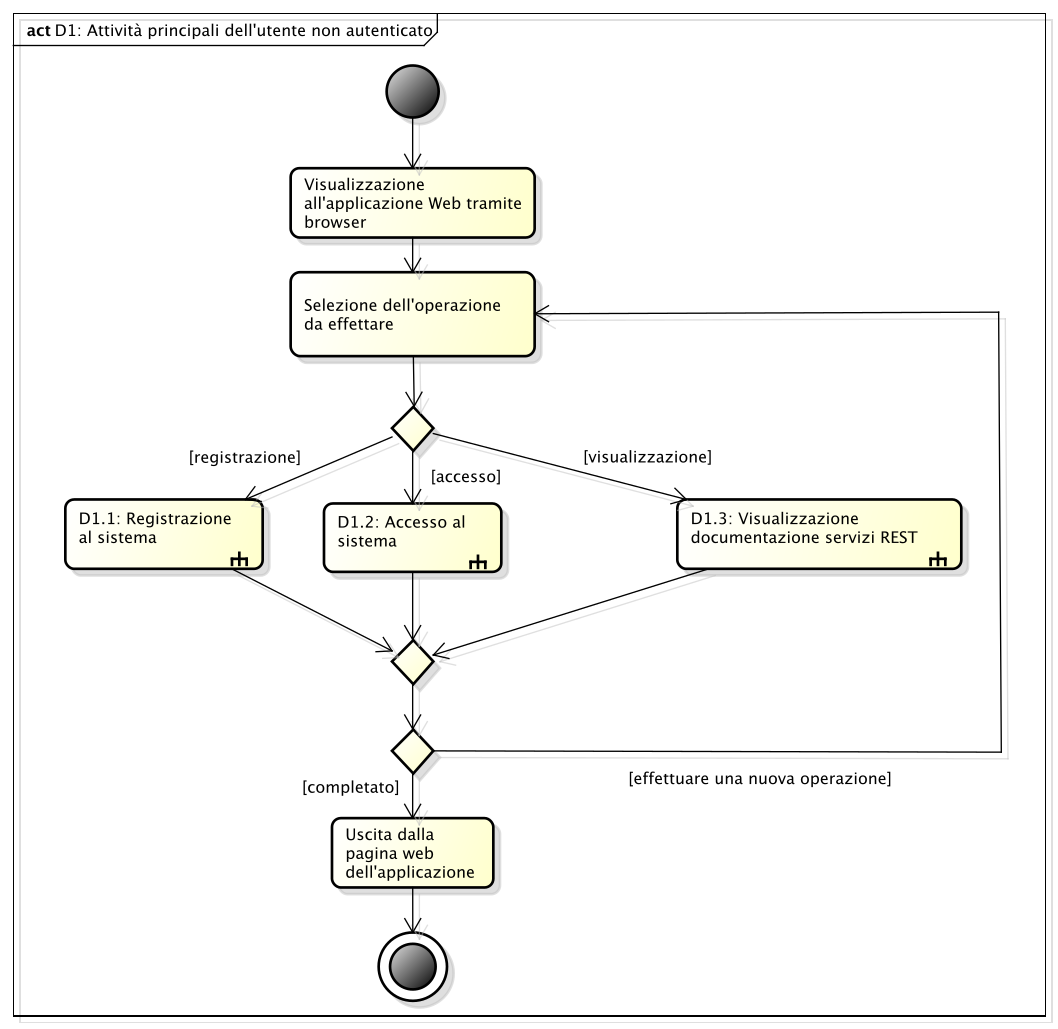
\includegraphics[scale=0.40]{./images/D1.pdf}}
			\caption{D1 - Diagramma delle attività principali dell'utente non autenticato}
		\end{figure}
		\noindent
		[TO DO] (descrizione generale e elenco delle attività principali)

		% subsubsection attività_principali_dell_utente_non_autenticato (end)

		\subsubsection{D1.1: Registrazione al sistema} % (fold)
		\label{ssub:registrazione_al_sistema}
		\begin{figure}[!htbp]
			\centering
			\centerline{\includegraphics[scale=0.45]{./images/D1_1.pdf}}
			\caption{D1.1 - Diagramma della registrazione al sistema}
		\end{figure}
		\noindent
		[TO DO] (descrizione generale)
		% subsubsection registrazione_al_sistema (end)

		\subsubsection{D1.2: Accesso al sistema} % (fold)
		\label{ssub:accesso_al_sistema}
		\begin{figure}[!htbp]
			\centering
			\centerline{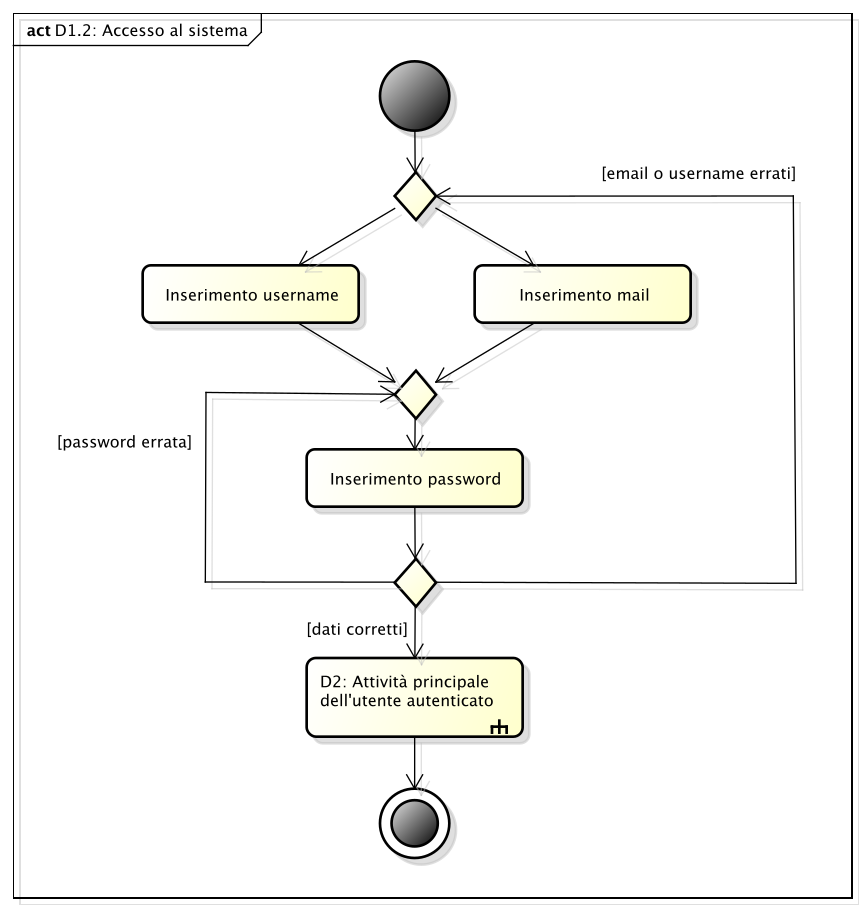
\includegraphics[scale=0.45]{./images/D1_2.pdf}}
			\caption{D1.2 - Diagramma dell'accesso al sistema}
		\end{figure}
		\noindent
		[TO DO] (descrizione generale) \newline

		% subsubsection accesso_al_sistema (end)

		\subsubsection{D1.3: Visualizzazione documentazione servizi REST} % (fold)
		\label{ssub:visualizzazione_documentazione_servizi_rest}
		\begin{figure}[!htbp]
			\centering
			\centerline{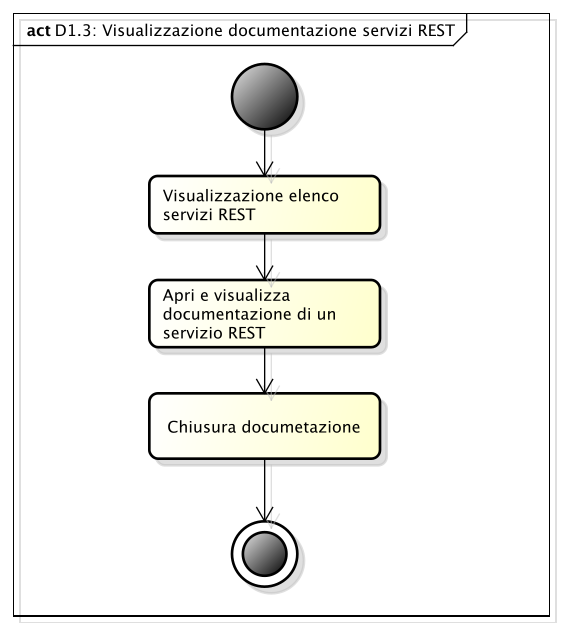
\includegraphics[scale=0.45]{./images/D1_3.pdf}}
			\caption{D1.3 - Diagramma della visualizzazione documentazione servizi REST}
		\end{figure}
		\noindent
		[TO DO] (descrizione generale)
		% subsubsection visualizzazione_documentazione_servizi_rest (end)

	% subsection utente_non_autenticato (end)

	\pagebreak
\clearpage \newpage

	\subsection{Utente autenticato} % (fold)
	\label{sub:utente_autenticato}
	In questa sezione vengono illustrate le attività che un utente autenticato al sistema può compiere.
		\subsubsection{D2: Attività principali dell'utente autenticato} % (fold)
		\label{ssub:attivita_principali_dell_utente_autenticato}
		\begin{figure}[!htbp]
			\centering
			\centerline{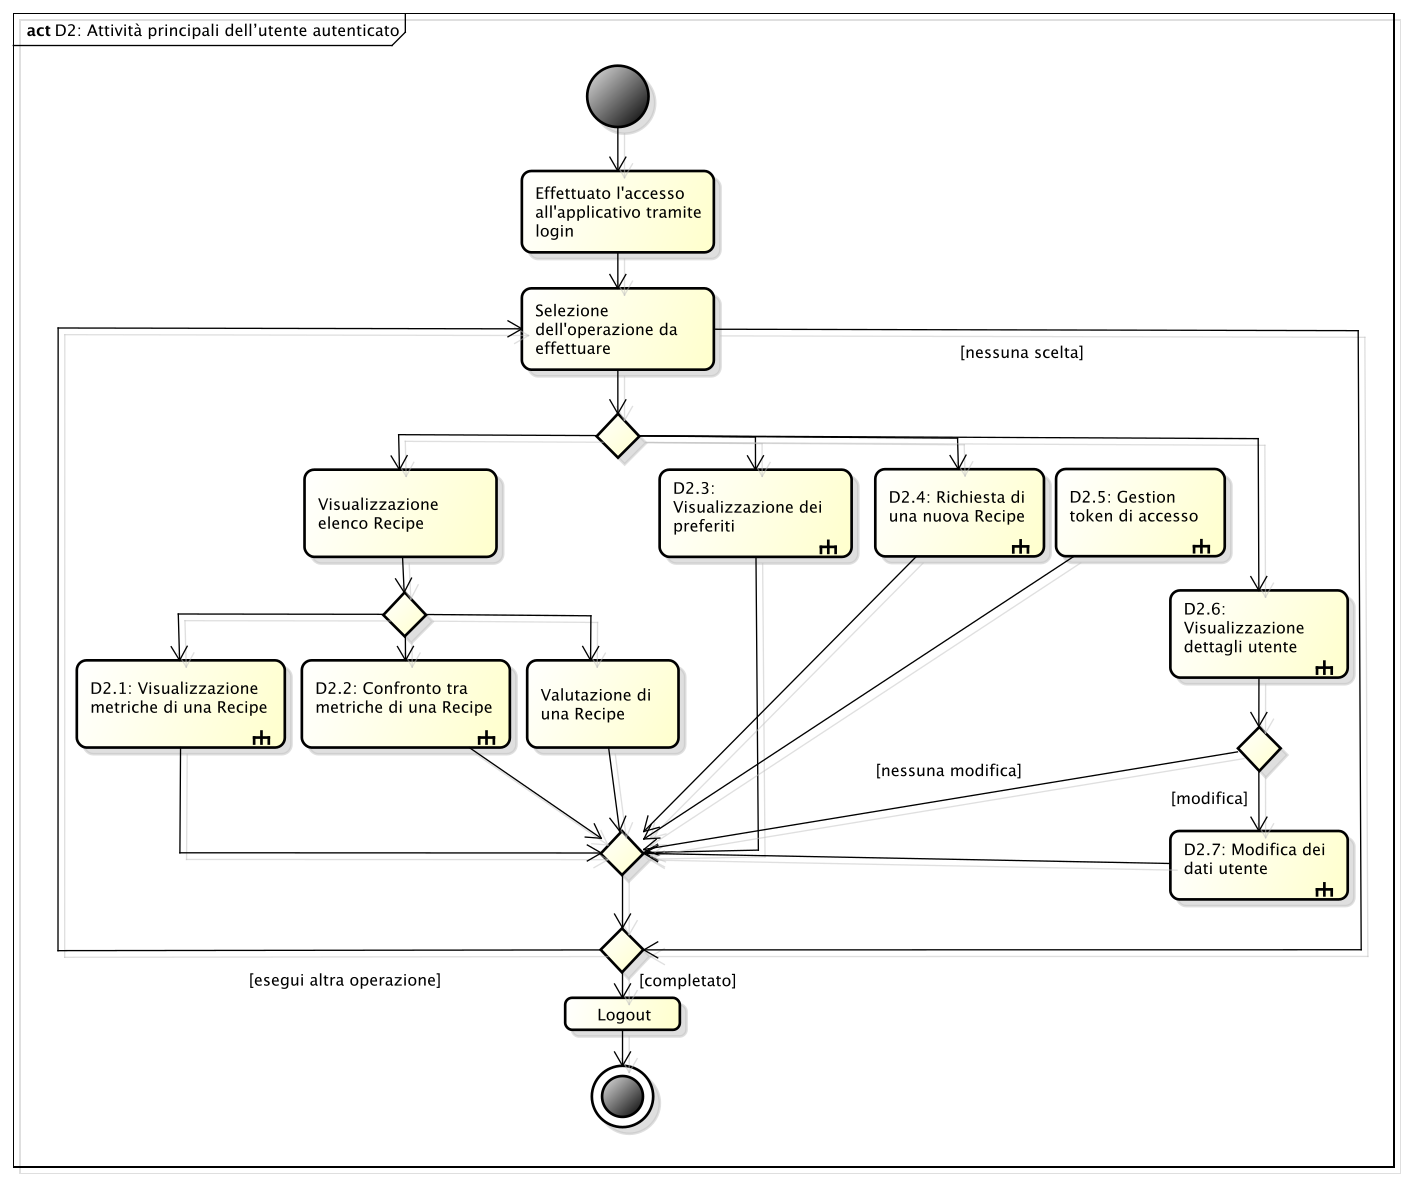
\includegraphics[scale=0.41]{./images/D2.pdf}}
			\caption{D2 - Diagramma delle attività principali dell'utente autenticato}
		\end{figure}
		\noindent
		[TO DO] (descrizione generale e elenco delle attività principali)
		% subsubsection attività_principali_dell_utente_autenticato (end)


		\subsubsection{D2.1: Visualizzazione metriche di una Recipe} % (fold)
		\label{ssub:visualizzazione_metriche_di_una_recipe}
		\label{ssub:registrazione_al_sistema}
		\begin{figure}[!htbp]
			\centering
			\centerline{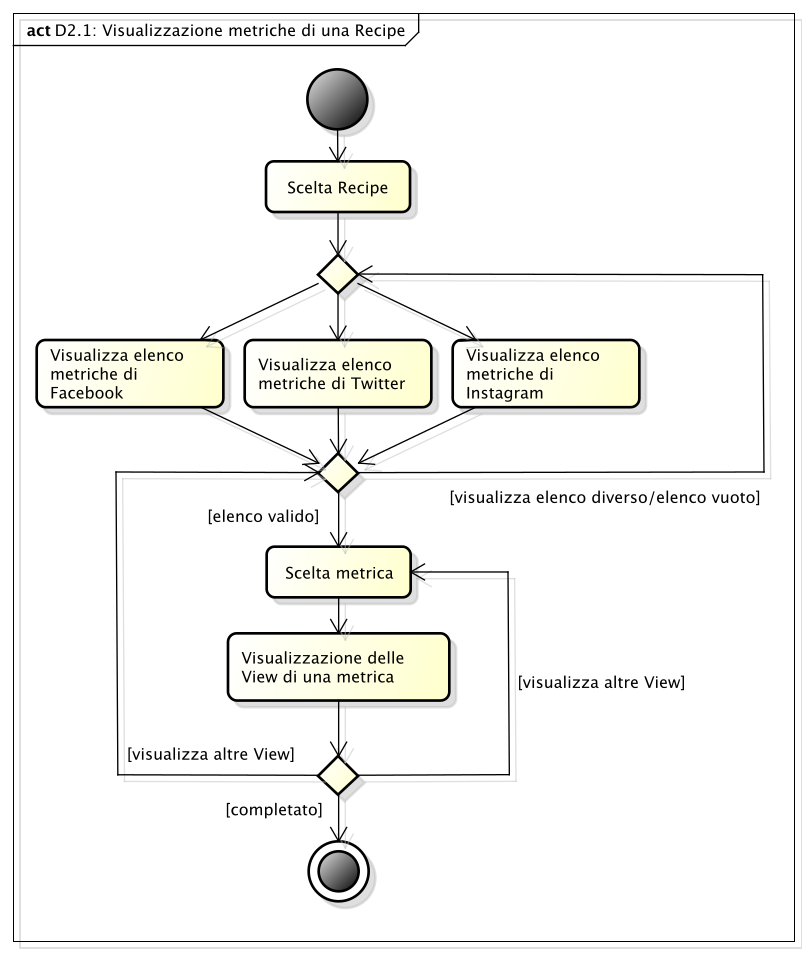
\includegraphics[scale=0.45]{./images/D2_1.pdf}}
			\caption{D2.1 - Diagramma della visualizzazione metriche di una Recipe}
		\end{figure}
		\noindent
		[TO DO] (descrizione generale)
		% subsubsection visualizzazione_metriche_di_una_recipe (end)


		\subsubsection{D2.2: Confronto tra metriche di una Recipe} % (fold)
		\label{ssub:confronto_tra_metriche_di_una_recipe}
		\begin{figure}[!htbp]
			\centering
			\centerline{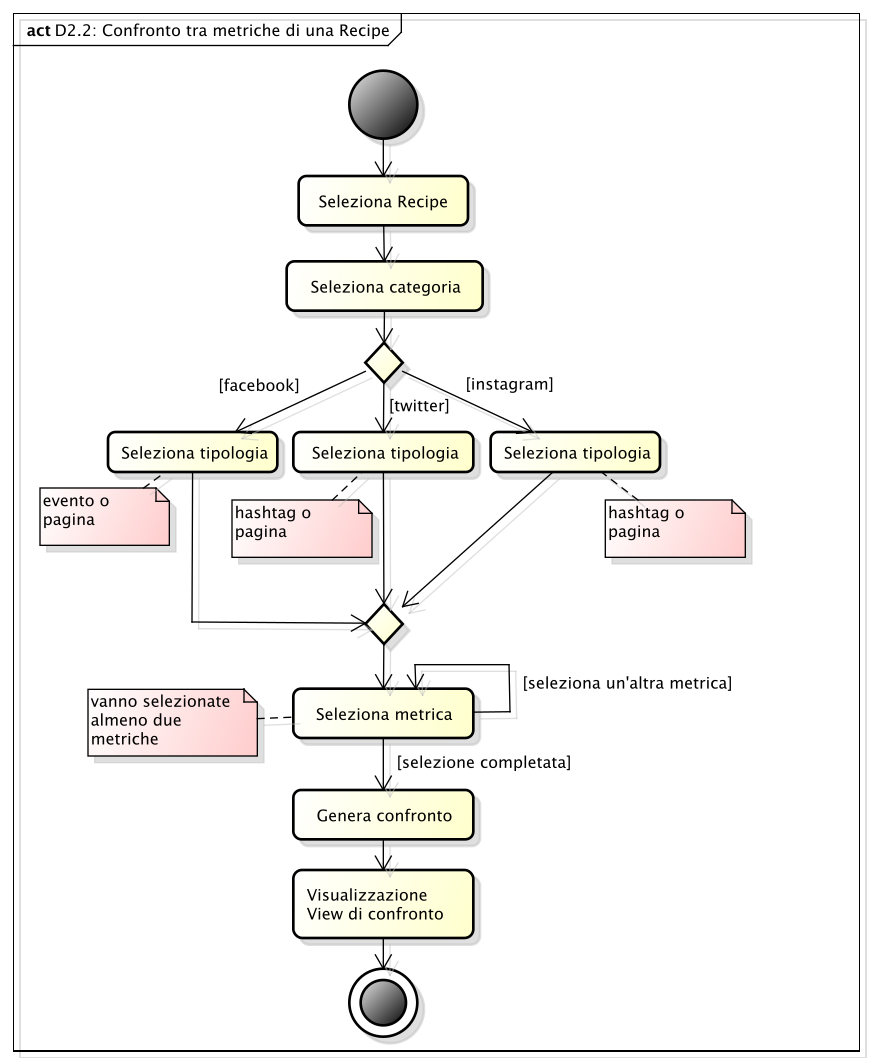
\includegraphics[scale=0.45]{./images/D2_2.pdf}}
			\caption{D2.2 - Diagramma del confronto tra metriche di una Recipe}
		\end{figure}
		\noindent
		[TO DO] (descrizione generale)
		% subsubsection confronto_tra_metriche_di_una_recipe (end)


		\subsubsection{D2.3: Richiesta di una nuova Recipe} % (fold)
		\label{ssub:richiesta_di_una_nuova_recipe}
		\begin{figure}[!htbp]
			\centering
			\centerline{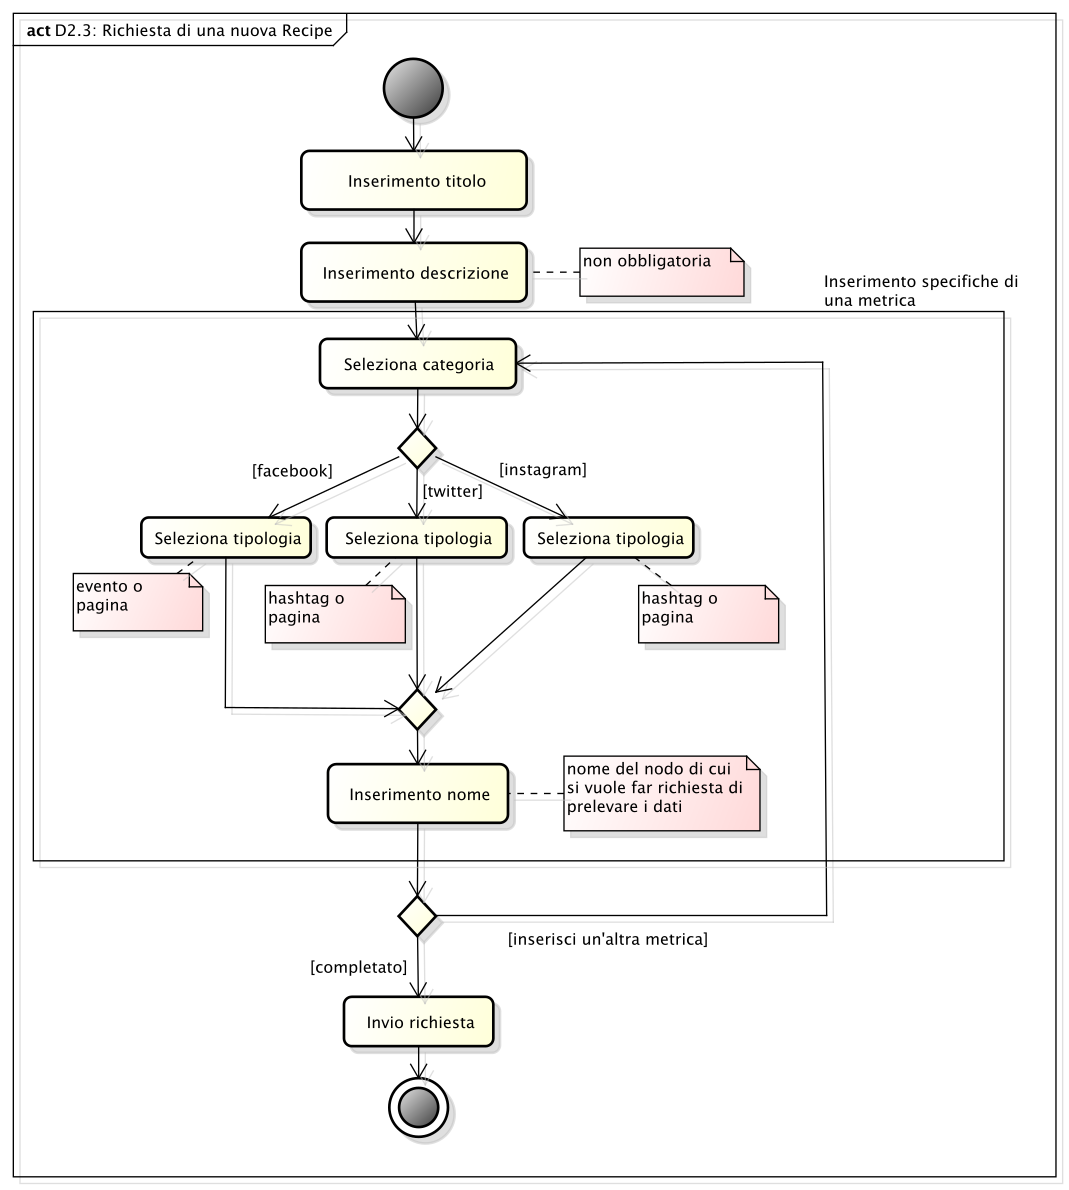
\includegraphics[scale=0.45]{./images/D2_3.pdf}}
			\caption{D2.3 - Diagramma della richiesta di una nuova Recipe}
		\end{figure}
		\noindent
		[TO DO] (descrizione generale)
		% subsubsection richiesta_di_una_nuova_recipe (end)

		\subsubsection{D2.4: Gestione token di accesso} % (fold)
		\label{ssub:gestione_token_di_accesso}
		\begin{figure}[!htbp]
			\centering
			\centerline{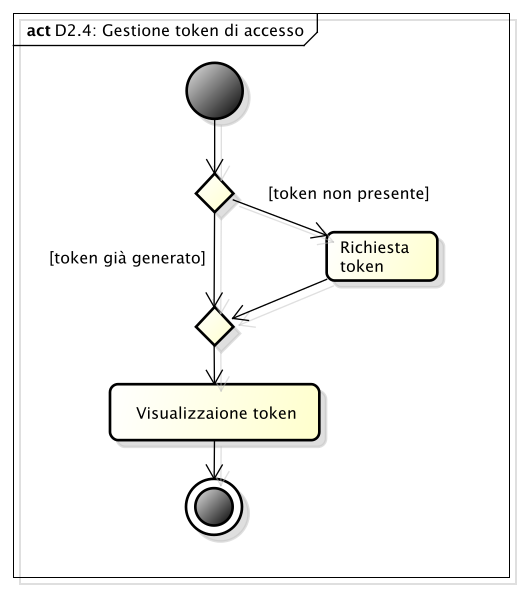
\includegraphics[scale=0.45]{./images/D2_4.pdf}}
			\caption{D2.4 - Diagramma della gestione del token di accesso}
		\end{figure}
		\noindent
		[TO DO] (descrizione generale)
		% subsubsection gestione_token_di_accesso (end)

		\subsubsection{D2.5: Visualizzazione dettagli utente} % (fold)
		\label{ssub:visualizzazione_dettagli_utente}
		\begin{figure}[!htbp]
			\centering
			\centerline{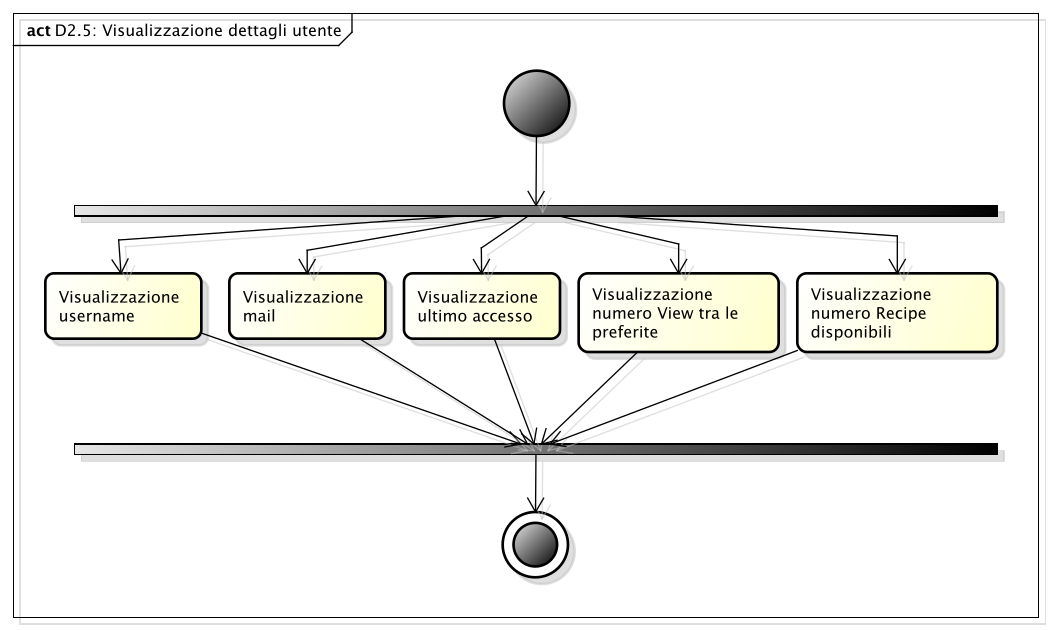
\includegraphics[scale=0.45]{./images/D2_5.pdf}}
			\caption{D2.5 - Diagramma della visualizzazione dettagli utente}
		\end{figure}
		\noindent
		[TO DO] (descrizione generale)
		% subsubsection visualizzazione_dettagli_utente (end)

		\subsubsection{D2.6: Modifica dei dati utente} % (fold)
		\label{ssub:modifica_dei_dati_utente}
		\begin{figure}[!htbp]
			\centering
			\centerline{\includegraphics[scale=0.45]{./images/UC1_1.pdf}}
			\caption{D2.6 - Diagramma della modifica dei dati utente}
		\end{figure}
		\noindent
		[TO DO] (descrizione generale)
		% subsubsection modifica_dei_dati_utente (end)

		\subsubsection{D2.6.1: Modifica della password} % (fold)
		\label{ssub:modifica_della_password}
		\begin{figure}[!htbp]
			\centering
			\centerline{\includegraphics[scale=0.45]{./images/UC1_1.pdf}}
			\caption{D2.6.1 - Diagramma della modifica della password}
		\end{figure}
		\noindent
		[TO DO] (descrizione generale)
		% subsubsection modifica_della_password (end)

	% subsection utente_autenticato (end)

	\pagebreak



	\subsection{Utente amministratore} % (fold)
	\label{sub:utente_amministratore}
	In questa sezione vengono illustrate le attività che un amministratore del sistema può compiere. L'utente amministratore oltre alle suddette potrà svolgere anche tutte le attività presenti nella sezione \ref{ssub:attivita_principali_dell_utente_autenticato}.
		\subsubsection{D3: Attività principali dell'utente amministratore} % (fold)
		\label{ssub:attivita_principali_dell_utente_amministratore}
		\begin{figure}[!htbp]
			\centering
			\centerline{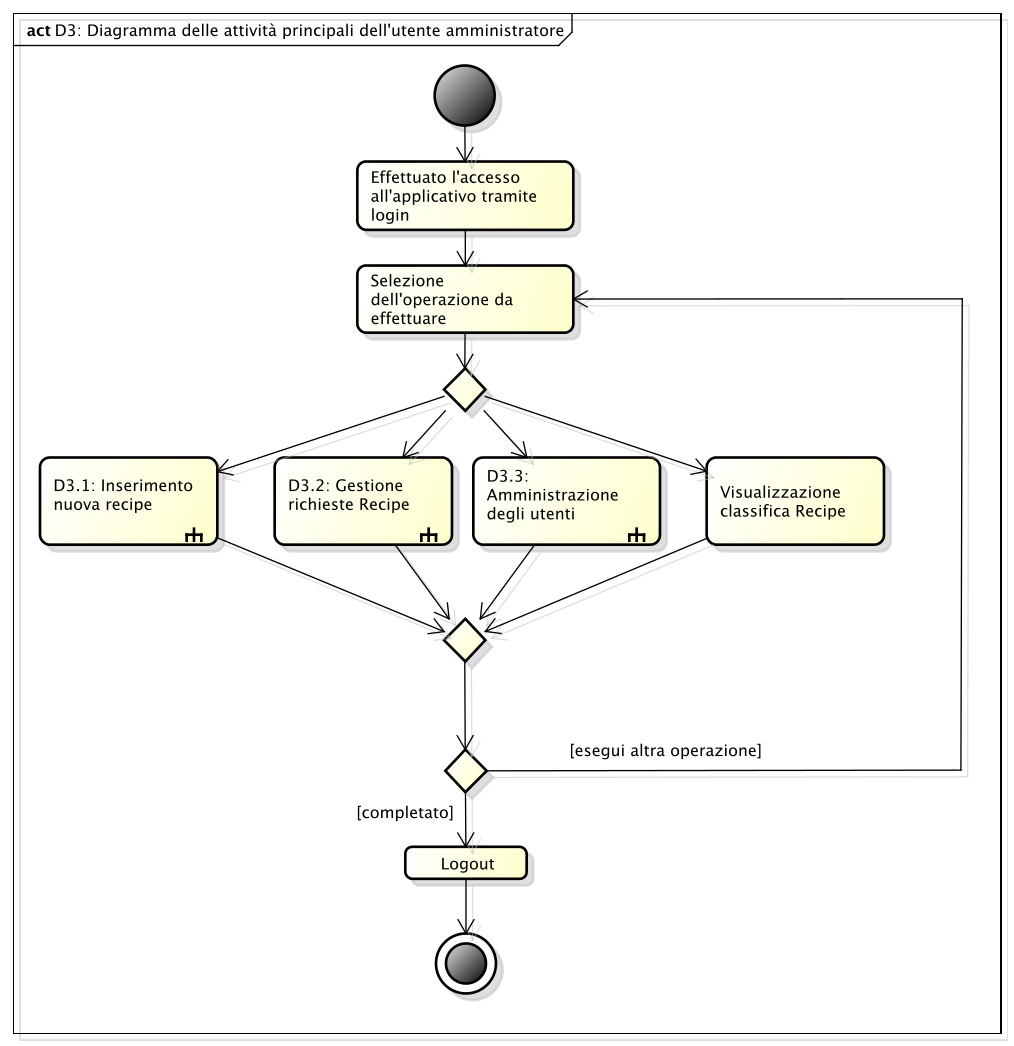
\includegraphics[scale=0.45]{./images/D3.pdf}}
			\caption{D3 - Diagramma delle attività principali dell'utente amministratore}
		\end{figure}
		\noindent
		[TO DO] (descrizione generale e elenco delle attività principali)

		% subsubsection attività_principali_dell_utente_amministratore (end)


		\subsubsection{D3.1: Inserimento nuova Recipe} % (fold)
		\label{ssub:inserimento_nuova_recipe}
		\begin{figure}[!htbp]
			\centering
			\centerline{\includegraphics[scale=0.45]{./images/UC1_1.pdf}}
			\caption{D3.1 - Diagramma dell'inserimento di una nuova Recipe}
		\end{figure}
		\noindent
		[TO DO] (descrizione generale)
		% subsubsection inserimento_nuova_recipe (end)


		\subsubsection{D3.2: Gestione richieste Recipe} % (fold)
		\label{ssub:gestione_richieste_recipe}
		\begin{figure}[!htbp]
			\centering
			\centerline{\includegraphics[scale=0.45]{./images/UC1_1.pdf}}
			\caption{D3.2 - Diagramma della gestione delle richieste Recipe}
		\end{figure}
		\noindent
		[TO DO] (descrizione generale)
		% subsubsection gestione_richieste_recipe (end)

		\subsubsection{D3.3: Amministrazione degli utenti} % (fold)
		\label{ssub:amministrazione_degli_utenti}
		\begin{figure}[!htbp]
			\centering
			\centerline{\includegraphics[scale=0.45]{./images/UC1_1.pdf}}
			\caption{D3.3 - Diagramma dell'amministrazione degli utenti}
		\end{figure}
		\noindent
		[TO DO] (descrizione generale)
		% subsubsection amministrazione_degli_utenti (end)




	% subsection utente_amministratore (end)




% section diagrammi_delle_attività (end) \clearpage \newpage
% =================================================================================================
% File:			design_pattern.tex
% Description:	Defiinisce la sezione relativa a ...
% Created:		2015-02-23
% Author:		Tesser Paolo
% Email:		tesser.paolo@mashup-unipd.it
% =================================================================================================
% Modification History:
% Version		Modifier Date		Change											Author
% 0.0.1 		2015-02-23 			sistemato header								Tesser Paolo
% =================================================================================================
% 0.0.2			2015-03-31			aggiunta introduzione ai DP						Tesser Paolo
% =================================================================================================
%


% CONTENUTO DEL CAPITOLO

\section{Design Pattern} % (fold)
\label{sec:design_pattern}
In questa sezione verranno presentati i diversi design pattern utilizzati per la progettazione architetturale. I design pattern sono soluzioni a problemi ricorrenti. Adottarli porta diversi benefici:
	\begin{itemize}
		\item favorisce il riutilizzo del codice;
		\item semplifica l’attività di progettazione;
		\item rende l’architettura più manutenibile.
	\end{itemize}
	\noindent
I design pattern possono essere suddivisi in:
	\begin{itemize}
		\item \textbf{Architetturali}: definiscono l’architettura dell’applicazione ad un livello elevato;
		\item \textbf{Creazionali}: permettono di nascondere i costruttori delle classi, consentendo la creazione di oggetti senza conoscerne la loro implementazione;
		\item \textbf{Strutturali}: consentono di riutilizzare classi preesistenti, fornendo un’interfaccia più adatta;
		\item \textbf{Comportamentali}: definiscono soluzioni per le interazioni tra oggetti.
	\end{itemize}
	\noindent
	\newline
Per una descrizione più approfondita dei design pattern utilizzati si faccia riferimento all’appendice \ref{sec:descdp}. I vari diagrammi che riprendono l’architettura non espongono tutte le sottoclassi e i metodi delle stesse. Lo scopo dei diagrammi è di mostrare le caratteristiche del design pattern adottato e come le varie classi interagiscono tra di loro. Nella realizzazione del progetto \projectName{} si è deciso di implementare i seguenti design pattern.

	\pagebreak

	% =================================================================================================
% File:			dp_architetturali.tex
% Description:	Defiinisce la sezione relativa a ...
% Created:		2015-03-26
% Author:		Tesser Paolo
% Email:		tesser.paolo@mashup-unipd.it
% =================================================================================================
% Modification History:
% Version		Modifier Date		Change											Author
% 0.0.1 		2015-03-26 			aggiunto sezioni								Tesser Paolo
% =================================================================================================
%
% =================================================================================================
%

% CONTENUTO DEL CAPITOLO

\subsection{Design pattern architetturali} % (fold)
\label{sub:design_pattern_architetturali}
[TO DO]
	\subsubsection{Three-Tier} % (fold)
	\label{ssub:three_tier}
	[TO DO]
	% subsubsection three_tier (end)

	\subsubsection{MVC} % (fold)
	\label{ssub:mvc}
	[TO DO]
	% subsubsection mvc (end)
% subsection design_pattern_architetturali (end) \clearpage \newpage
	% =================================================================================================
% File:			dp_creazionali.tex
% Description:	Defiinisce la sezione relativa a ...
% Created:		2015-03-26
% Author:		Tesser Paolo
% Email:		tesser.paolo@mashup-unipd.it
% =================================================================================================
% Modification History:
% Version		Modifier Date		Change											Author
% 0.0.1 		2015-03-26 			creato scheltro sezione							Tesser Paolo
% =================================================================================================
% 0.0.2			2015-04-08			inserito scheletro per DP: Prototype e Module	Tesser Paolo
% =================================================================================================
% 0.0.3			2015-04-14			descritto Prototype, Module e Constructor		Tesser Paolo
% =================================================================================================
%

% CONTENUTO DEL CAPITOLO

\subsection{Design pattern creazionali} % (fold)
\label{sub:design_pattern_creazionali}

	\subsubsection{Constructor Pattern} % (fold)
	\label{ssub:constructor_pattern}
		\begin{itemize}
			\item \textbf{Scope dell'utilizzo}: questo pattern è utilizzato per emulare il costruttore tipico della programmazione ad oggetti attraverso delle funzioni che lavorano con gli oggetti;
			\item \textbf{Contesto dell'utilizzo}:
				\begin{itemize}
					\item \textbf{Client}: viene utilizzato in tutte le classi del package \texttt{client::model}. \newline
					Non è possibile fornirne una rappresentazione grafica in quanto questo pattern viene realizzato durante la codifica effettiva delle componenti.
				\end{itemize}
		\end{itemize}
	% subsubsection constructor_pattern (end)

	\subsubsection{Prototype Pattern} % (fold)
	\label{ssub:prototype_pattern}
		\begin{itemize}
			\item \textbf{Scope dell'utilizzo}: questo pattern è utilizzato per generare il meccanismo di ereditarietà tra due classi. Viene anche scelto in modo che i metodi di una classe siano condivisi tra i diversi oggetti in quanto altrimenti, in JavaScript, siccome non è presente il concetto di classi si andrebbe a ripetere un metodo ogni volta che si istanzia un nuovo oggetto e questo non è ottimale;
			\item \textbf{Contesto dell'utilizzo}:
				\begin{itemize}
					\item \textbf{Client}: viene utilizzato nelle classi del package \texttt{client::model} ad esempio tra \texttt{UserModel} e \texttt{UserAdminModel}. \newline
					Non è possibile fornirne una rappresentazione grafica in quanto questo pattern viene realizzato durante la codifica effettiva delle componenti.
				\end{itemize}
		\end{itemize}
	% subsubsection prototype_pattern (end)

	\subsubsection{Module Pattern} % (fold)
	\label{ssub:module_pattern}
		\begin{itemize}
			\item \textbf{Scope dell'utilizzo}: questo pattern serve per garantire, in particolare in JavaScript, l'incapsulamento e la privacy. \'E quindi utilizzato principalmente quando si vuole emulare il concetto di classe, definendo dei membri e dei metodi sia privati che pubblici;
			\item \textbf{Contesto dell'utilizzo}:
				\begin{itemize}
					\item \textbf{Client}: viene utilizzato in tutte le classi del package \texttt{client::model::data} per incapsulare al meglio i membri e i metodi che i modelli dei dati usano. \newline
					Non è possibile fornirne una rappresentazione grafica in quanto questo pattern viene realizzato durante la codifica effettiva delle componenti.
				\end{itemize}
		\end{itemize}
	% subsubsection module_pattern (end)

	\subsubsection{Singleton} % (fold)
	\label{ssub:singleton}
		\begin{itemize}
			\item \textbf{Scope dell'utilizzo}: questo pattern è utilizzato per limitare l'instaziazione di un certo tipo classe ad un solo oggetto in modo tale che esso rimanga unico nel sistema in cui risiede;
			\item \textbf{Contesto dell'utilizzo}:
				\begin{itemize}
					\item \textbf{Client}: viene utilizzato direttamente da AngularJS quando si utilizzano i ``service'' o i ``factory'', utilizzati per creare la logica di business del front-end nel package \texttt{client::model}. Il framework gestisce internamente questo pattern attraverso una hash map che risiede nella cache. Essa rappresenta un singleton manager che detiene le dipendenze che vengono istanziate e le restituisce quando richieste senza crearne una nuova se questa esiste già. \newline
					Non ne viene fornita nessuna rappresentazione grafica in quanto non è una cosa che viene progettata dal team, ma usata direttamente attraverso il framework scelto;
					\item \textbf{Server}: viene utilizzato dalla classe \texttt{server::endpoints::RequestHandler} in quanto quest'ultima, essendo implementata secondo il pattern Front Controller, rappresenta il punto di accesso comune a tutto il sistema in cui confluiscono le richieste provenienti dalle classi appartenenti al package \texttt{server::endpoints} (\ref{ssub:bdsm_app_server_endpoints}). \newline
					[TO DO] (grafico del pattern applicato al caso di utilizzo nell'applicativo)
				\end{itemize}
		\end{itemize}
	% subsubsection singleton (end)
% subsection design_pattern_creazionali (end)
 \clearpage \newpage
	% =================================================================================================
% File:			dp_strutturali.tex
% Description:	Defiinisce la sezione relativa a ...
% Created:		2015-03-26
% Author:		Tesser Paolo
% Email:		tesser.paolo@mashup-unipd.it
% =================================================================================================
% Modification History:
% Version		Modifier Date		Change											Author
% 0.0.1 		2015-03-26 			sistemato header								Tesser Paolo
% =================================================================================================
% 0.0.2			2015-04-08			aggiunto scheletro per pattern Facade			Tesser Paolo
% =================================================================================================
% 0.0.3			2015-04-13			descritto pattern Facade						Tesser Paolo
% =================================================================================================
%

% CONTENUTO DEL CAPITOLO

\subsection{Design pattern strutturali} % (fold)
\label{sub:design_pattern_strutturali}
	\subsubsection{Fa\c{c}ade} % (fold)
	\label{ssub:facade}
		\begin{itemize}
			\item \textbf{Scope dell'utilizzo}: questo pattern è utilizzato per fornire un'interfaccia di alto livello unificata di tante interfacce di un sotto sistema più complesso. Questo rende più semplice al client interagire con quel sistema senza preoccuparsi di come le cose vengono implementate da esso;
			\item \textbf{Contesto dell'utilizzo}:
				\begin{itemize}
					\item \textbf{Client}: viene utilizzato direttamente da AngularJS in alcuni servizi come quello \$http o \$resource che permettono all'utilizzatore di non sapere come viene effettivamente implementata la chiamata alle API, effettuandola quindi in maniera più semplice di come è realmente. \newline
					Non ne viene fornita nessuna rappresentazione grafica in quanto non è una cosa che viene progettata dal team, ma usata direttamente attraverso il framework scelto.
				\end{itemize}
		\end{itemize}
	% subsubsection facade (end)


	\subsubsection{Front controller} % (fold)
	\label{ssub:front_controller}
		\begin{itemize}
			\item \textbf{Scope dell'utilizzo}: [TO DO];
			\item \textbf{Contesto dell'utilizzo}:
				\begin{itemize}
					\item \textbf{Server}: [TO DO]. \newline
					[TO DO] (grafico del pattern applicato al caso di utilizzo nell'applicativo)
				\end{itemize}
		\end{itemize}
		% subsubsection front_controller (end)



% subsection design_pattern_strutturali (end) \clearpage \newpage
	% =================================================================================================
% File:			dp_comportamentali.tex
% Description:	Defiinisce la sezione relativa a ...
% Created:		2015-03-26
% Author:		Tesser Paolo
% Email:		tesser.paolo@mashup-unipd.it
% =================================================================================================
% Modification History:
% Version		Modifier Date		Change											Author
% 0.0.1 		2015-03-26 			sistemato header								Tesser Paolo
% =================================================================================================
%
% =================================================================================================
%

% CONTENUTO DEL CAPITOLO

\subsection{Design pattern comportamentali} % (fold)
\label{sub:design_pattern_comportamentali}
[TO DO]
% subsection design_pattern_comportamentali (end) \clearpage \newpage
% section design_pattern (end)
 \clearpage \newpage
% =================================================================================================
% File:			stime_fattibilita.tex
% Description:	Defiinisce la sezione relativa a ...
% Created:		2015-02-23
% Author:		Tesser Paolo
% Email:		tesser.paolo@mashup-unipd.it
% =================================================================================================
% Modification History:
% Version		Modifier Date		Change											Author
% 0.0.1 		2015-02-23 			sistemato header								Tesser Paolo
% =================================================================================================
%
% =================================================================================================
%

% CONTENUTO DEL CAPITOLO

\section{Stime di fattibilità} % (fold)
\label{sec:stime_di_fattibilita}

% section stime_di_fattibilità (end) \clearpage \newpage
% =================================================================================================
% File:			tracciamento.tex
% Description:	Defiinisce la sezione relativa al capitolo di tracciamento dei requisiti con le classi
% Created:		2015-04-21
% Author:		Tesser Paolo
% Email:		tesser.paolo@mashup-unipd.it
% =================================================================================================
% Modification History:
% Version		Modifier Date		Change											Author
% 0.0.1 		2015-04-21 			creato scheletro doc							Tesser Paolo
% =================================================================================================
%

% CONTENUTO DEL CAPITOLO

\section{Tracciamento} % (fold)
\label{sec:tracciamento}
	\subsection{Classi-Requisiti} % (fold)
\label{sub:classi_requisiti}
\begin{center}
\def\arraystretch{1.5}
\bgroup
\begin{longtable}{| p{11cm} | p{2.5cm} |}
\hline
\textbf{Classi} & \textbf{Requisiti} \\
\hline
client::model::data::ViewTypeModel & ROF5.3 \\
\hline
client::model::data::ApiDocsModel & ROF11 \\
\hline
client::model::data::UserModel & TO DO: Requisito non tracciato con nessun componente! \\
\hline
client::model::data::RecipeModel & TO DO: Requisito non tracciato con nessun componente! \\
\hline
client::model::data::RecipeRequestModel & TO DO: Requisito non tracciato con nessun componente! \\
\hline
client::model::data::RecipeInsertModel & TO DO: Requisito non tracciato con nessun componente! \\
\hline
client::model::data::MetricModel & TO DO: Requisito non tracciato con nessun componente! \\
\hline
client::model::data::CompareModel & TO DO: Requisito non tracciato con nessun componente! \\
\hline
client::model::services::AuthServiceTarget & ROF4.1.1.1 \newline ROF4.1.2 \\
\hline
client::model::services::AuthServiceAdapter & TO DO: Requisito non tracciato con nessun componente! \\
\hline
client::model::services::RecipeService & ROF5.1 \newline ROF5.1.1 \newline ROF5.2 \newline RDF6 \newline RDF6.1 \newline RDF6.2 \newline RDF6.2.2 \newline RDF6.3 \newline RDF6.3.1 \newline RFF7.1.1.4 \newline RFF7.1.1.5 \newline RFF7.1.1.6 \newline RFF7.1.1.7 \newline RFF8.4 \\
\hline
client::model::services::RecipeAdminService & RFF10 \newline RFF10.2 \\
\hline
client::model::services::UserService & ROF3.3.1 \newline ROF3.3.7.2.1 \\
\hline
client::model::services::UserAdminService & RFF9.1.1 \newline RFF9.2.1 \newline ROF9.3.1 \newline ROF9.3.2 \\
\hline
client::model::services::ChartCreator & ROF5.3 \newline ROF5.4 \newline ROF5.5 \newline ROF5.6.4.2 \\
\hline
client::model::services::LineChartCreator & ROF5.3.1 \newline ROF5.3.1.1 \newline ROF5.4.1 \newline ROF5.4.1.2 \newline ROF5.4.1.4 \newline ROF5.5.1 \newline ROF5.5.1.2 \newline ROF5.5.1.3 \newline ROF5.5.1.4 \newline ROF5.5.1.5 \newline ROF5.5.1.7 \newline ROF5.5.1.8 \newline ROF5.6.4.1.2 \newline ROF5.6.4.1.3 \newline ROF5.6.4.1.4 \newline ROF5.6.4.1.5 \newline ROF5.6.4.1.6 \\
\hline
client::model::services::BarChartCreator & ROF5.3.1 \newline ROF5.3.1.6 \newline ROF5.4.1 \newline ROF5.4.1.1 \newline ROF5.5.1 \newline ROF5.5.1.1 \newline ROF5.6.4.1.2 \newline ROF5.6.4.1.3 \newline ROF5.6.4.1.4 \newline ROF5.6.4.1.5 \newline ROF5.6.4.1.6 \\
\hline
client::model::services::PieChartCreator & ROF5.3.1 \newline ROF5.3.1.2 \newline ROF5.3.1.3 \newline ROF5.3.1.4 \newline ROF5.4.1 \newline ROF5.4.1.5 \newline ROF5.4.1.7 \newline ROF5.5.1 \newline ROF5.5.1.10 \newline ROF5.6.4.1.1 \newline ROF5.6.4.1.2 \newline ROF5.6.4.1.3 \newline ROF5.6.4.1.4 \newline ROF5.6.4.1.5 \newline ROF5.6.4.1.6 \\
\hline
client::model::services::MapChartCreator & ROF5.3.1 \newline ROF5.3.1.5 \newline ROF5.4.1 \newline ROF5.4.1.3 \newline ROF5.5.1 \newline ROF5.5.1.9 \\
\hline
client::model::services::RadarChartCreator & ROF5.4.1 \newline ROF5.4.1.6 \newline ROF5.5.1 \newline ROF5.5.1.6 \\
\hline
client::model::services::DataManagerService & ROF5.1 \newline ROF5.2 \newline RDF6.1 \newline RDF6.2 \newline RFF9.1.1 \newline RFF9.2.1 \\
\hline
client::view::public::Login & ROF2 \newline ROF2.1 \newline ROF2.2 \newline ROF2.3 \newline ROF2.4 \newline ROF2.4.1 \newline ROF2.4.2 \newline ROF3.3.7.2.2 \\
\hline
client::view::public::About & TO DO: Requisito non tracciato con nessun componente! \\
\hline
client::view::public::Register & ROF1 \newline ROF1.1 \newline ROF1.2 \newline ROF1.3 \newline ROF1.4 \newline RDF1.5 \newline ROF1.6 \newline ROF1.7 \\
\hline
client::view::public::ApiDocs & ROF11 \newline ROF12.1 \newline ROF12.1.1 \newline ROF12.1.2 \newline ROF12.1.3 \newline ROF12.2 \\
\hline
client::view::user::Home & ROF2.5 \newline ROF4 \newline ROF4.1.1.1 \newline ROF4.1.2 \\
\hline
client::view::user::Recipe & ROF2.5 \newline ROF5 \newline ROF5.1 \newline ROF5.1.1 \newline ROF5.1.2 \newline RFF5.1.3 \newline RFF5.1.3.2 \newline ROF8.3 \newline ROF8.3.1 \\
\hline
client::view::user::Metrics & ROF5.2 \newline ROF5.2.1 \newline ROF5.2.1.2 \newline ROF5.2.1.3 \\
\hline
client::view::user::Charts & ROF5.2.2 \newline ROF5.3 \newline ROF5.3.1.1 \newline ROF5.3.1.2 \newline ROF5.3.1.3 \newline ROF5.3.1.4 \newline ROF5.3.1.5 \newline ROF5.3.1.6 \newline ROF5.4 \newline ROF5.4.1.1 \newline ROF5.4.1.2 \newline ROF5.4.1.3 \newline ROF5.4.1.4 \newline ROF5.4.1.5 \newline ROF5.4.1.6 \newline ROF5.4.1.7 \newline ROF5.5 \newline ROF5.5.1.1 \newline ROF5.5.1.2 \newline ROF5.5.1.3 \newline ROF5.5.1.4 \newline ROF5.5.1.5 \newline ROF5.5.1.6 \newline ROF5.5.1.7 \newline ROF5.5.1.8 \newline ROF5.5.1.9 \newline ROF5.5.1.10 \newline RDF6.2 \newline RDF6.2.1 \newline RDF6.2.2 \\
\hline
client::view::user::Compare & ROF5.6 \newline ROF5.6.1 \newline ROF5.6.2 \newline ROF5.6.2.1 \newline ROF5.6.2.2 \newline ROF5.6.2.3 \newline ROF5.6.3 \newline ROF5.6.3.1 \newline ROF5.6.4 \newline ROF5.6.4.1 \newline ROF5.6.4.1.1 \newline ROF5.6.4.1.2 \newline ROF5.6.4.1.3 \newline ROF5.6.4.1.4 \newline ROF5.6.4.1.5 \newline ROF5.6.4.1.6 \newline ROF5.6.4.2 \newline ROF5.6.4.3 \\
\hline
client::view::user::RecipeRequest & RFF7 \newline RFF7.1 \newline RFF7.1.1 \newline RFF7.1.1.1 \newline RFF7.1.1.2 \newline RFF7.1.1.3 \newline RFF7.1.1.4 \newline RFF7.1.1.5 \newline RFF7.1.1.6 \newline RFF7.1.1.7 \newline RFF7.1.1.8 \newline RFF7.1.1.9 \newline RFF7.1.1.10 \newline RFF7.1.1.11 \newline RFF7.1.1.12 \newline RFF7.1.2 \newline RFF7.1.3 \\
\hline
client::view::user::Favourites & RDF6.1 \newline RDF6.1.1 \newline RDF6.3 \newline RDF6.3.1 \\
\hline
client::view::user::TokenConfig & ROF11 \newline ROF11.1.1 \newline ROF11.1.2 \newline ROF11.2.2 \newline ROF11.2.3 \newline ROF11.3.1 \newline ROF11.3.2 \newline ROF12 \newline ROF12.1 \newline ROF12.1.1 \newline ROF12.1.2 \newline ROF12.1.3 \newline ROF12.2 \\
\hline
client::view::user::Settings & ROF3.1 \newline ROF3.1.1 \newline ROF3.1.2 \newline ROF3.1.3 \newline RFF3.1.4 \newline ROF3.3 \newline ROF3.3.1 \newline ROF3.3.2 \newline ROF3.3.2.1 \newline ROF3.3.2.2 \newline ROF3.3.3 \newline ROF3.3.3.1 \newline ROF3.3.3.2 \newline ROF3.3.3.3 \newline ROF3.3.4 \newline ROF3.3.4.1 \newline ROF3.3.4.2 \newline ROF3.3.4.2.1 \newline ROF3.3.4.3 \newline ROF3.3.4.3.1 \newline RDF3.3.5 \newline ROF3.3.6 \newline ROF3.3.6.2 \newline ROF3.3.6.3 \newline ROF3.3.7 \newline ROF3.3.7.1 \newline ROF3.3.7.2 \\
\hline
client::view::user::Menu & TO DO: Requisito non tracciato con nessun componente! \\
\hline
client::view::user::MenuMain & ROF3 \newline ROF4 \newline ROF4.1.1 \newline ROF12 \\
\hline
client::view::user::MenuSecond & ROF3 \\
\hline
client::view::admin::RecipeConfig & ROF8.1 \\
\hline
client::view::admin::RequestList & RFF10 \newline RFF10.1 \newline RFF10.1.1 \newline RFF10.1.2 \newline RFF10.2 \newline RFF10.3 \newline RFF10.3.1 \newline RFF10.3.2 \newline RFF10.3.2.1 \newline RFF10.4 \newline RFF10.5 \newline RFF10.5.1 \\
\hline
client::view::admin::Insert & ROF8.1 \newline ROF8.1.1 \newline ROF8.1.1.1 \newline ROF8.1.1.2 \newline ROF8.1.1.3 \newline ROF8.1.1.4 \newline ROF8.2 \newline ROF8.2.1 \\
\hline
client::view::admin::Ratings & RFF8.4 \newline RFF8.4.1 \newline RFF8.4.2 \\
\hline
client::view::admin::UsersConfig & TO DO: Requisito non tracciato con nessun componente! \\
\hline
client::view::admin::MenuSecondAdmin & ROF8 \newline ROF9 \\
\hline
client::controller::public::PublicRoute & ROF1 \newline ROF2 \newline ROF3.3.7.2.2 \\
\hline
client::controller::public::LoginCtrl & ROF2 \newline ROF2.1 \newline ROF2.2 \newline ROF2.3 \newline ROF2.4 \newline ROF2.4.1 \newline ROF2.4.2 \newline ROF3.3.7.2.2 \\
\hline
client::controller::public::RegisterCtrl & ROF1 \newline ROF1.1 \newline ROF1.2 \newline ROF1.3 \newline ROF1.4 \newline RDF1.5 \newline ROF1.6 \newline ROF1.7 \\
\hline
client::controller::public::ApiDocsCtrl & TO DO: Requisito non tracciato con nessun componente! \\
\hline
client::controller::user::MenuCtrl & TO DO: Requisito non tracciato con nessun componente! \\
\hline
client::controller::user::MenuMainCtrl & ROF4 \newline ROF4.1 \\
\hline
client::controller::user::MenuSecondCtrl & ROF8 \\
\hline
client::controller::user::HomeRoute & ROF2.5 \\
\hline
client::controller::user::HomeCtrl & ROF4 \newline ROF4.1 \\
\hline
client::controller::user::RecipeRoute & ROF2.5 \\
\hline
client::controller::user::RecipeCtrl & ROF5 \newline ROF5.1 \newline ROF5.1.1 \newline RFF5.1.3.1 \newline RFF5.1.3.2 \newline ROF8.3 \\
\hline
client::controller::user::MetricsCtrl & ROF5.2 \newline ROF5.2.1.2 \\
\hline
client::controller::user::ChartsCtrl & ROF5.2.2 \newline ROF5.3.1.1 \newline ROF5.3.1.2 \newline ROF5.3.1.3 \newline ROF5.3.1.4 \newline ROF5.3.1.5 \newline ROF5.3.1.6 \newline ROF5.4 \newline ROF5.4.1.1 \newline ROF5.4.1.2 \newline ROF5.4.1.3 \newline ROF5.4.1.4 \newline ROF5.4.1.5 \newline ROF5.4.1.6 \newline ROF5.4.1.7 \newline ROF5.5 \newline ROF5.5.1.1 \newline ROF5.5.1.2 \newline ROF5.5.1.3 \newline ROF5.5.1.4 \newline ROF5.5.1.5 \newline ROF5.5.1.6 \newline ROF5.5.1.7 \newline ROF5.5.1.8 \newline ROF5.5.1.9 \newline ROF5.5.1.10 \newline RDF6.2 \\
\hline
client::controller::user::CompareCtrl & ROF5.6 \newline ROF5.6.4 \newline ROF5.6.4.1 \newline ROF5.6.4.1.1 \newline ROF5.6.4.1.2 \newline ROF5.6.4.3 \\
\hline
client::controller::user::RecipeRequestRoute & RFF7 \\
\hline
client::controller::user::RecipeRequestCtrl & RFF7 \newline RFF7.1 \newline RFF7.1.1 \newline RFF7.1.1.1 \newline RFF7.1.1.2 \newline RFF7.1.1.3 \newline RFF7.1.1.4 \newline RFF7.1.1.5 \newline RFF7.1.1.6 \newline RFF7.1.1.7 \newline RFF7.1.1.8 \newline RFF7.1.1.9 \newline RFF7.1.1.10 \newline RFF7.1.2 \newline RFF7.1.3 \\
\hline
client::controller::user::FavouritesRoute & RDF6 \\
\hline
client::controller::user::FavouritesCtrl & RDF6.1 \newline RDF6.1.1 \newline RDF6.3 \newline RDF6.3.1 \\
\hline
client::controller::user::TokenConfigRoute & ROF12 \\
\hline
client::controller::user::TokenConfigCtrl & ROF11.1 \newline ROF11.1.1 \newline ROF11.1.2 \newline ROF11.2 \newline ROF11.3.1 \newline ROF11.3.2 \\
\hline
client::controller::user::SettingsRoute & ROF3.1 \newline ROF3.1.1 \newline ROF3.1.2 \newline ROF3.1.3 \newline RFF3.1.4 \\
\hline
client::controller::user::SettingsCtrl & ROF3.1 \newline ROF3.1.1 \newline ROF3.1.2 \newline ROF3.1.3 \newline RFF3.1.4 \newline ROF3.3 \newline ROF3.3.1 \newline ROF3.3.2 \newline ROF3.3.2.1 \newline ROF3.3.2.2 \newline ROF3.3.3 \newline ROF3.3.3.1 \newline ROF3.3.3.2 \newline ROF3.3.3.3 \newline ROF3.3.4 \newline ROF3.3.4.1 \newline ROF3.3.4.2 \newline ROF3.3.4.2.1 \newline ROF3.3.4.3 \newline ROF3.3.4.3.1 \newline RDF3.3.5 \newline ROF3.3.6 \newline ROF3.3.6.2 \newline ROF3.3.6.3 \newline ROF3.3.7 \newline ROF3.3.7.1 \newline ROF3.3.7.2 \\
\hline
client::controller::user::LogoutCtrl & TO DO: Requisito non tracciato con nessun componente! \\
\hline
client::controller::admin::MenuSecondAdminCtrl & ROF8 \\
\hline
client::controller::admin::RecipeConfigRoute & ROF8 \newline ROF8.1 \\
\hline
client::controller::admin::RecipeConfigCtrl & ROF8.1 \\
\hline
client::controller::admin::RequestListRoute & ROF8 \newline RFF10 \\
\hline
client::controller::admin::RequestListCtrl & RFF10 \newline RFF10.1 \newline RFF10.1.1 \newline RFF10.1.2 \newline RFF10.2 \newline RFF10.3 \newline RFF10.3.1 \newline RFF10.3.2 \newline RFF10.3.2.1 \newline RFF10.4 \newline RFF10.5 \newline RFF10.5.1 \\
\hline
client::controller::admin::InsertRecipeCtrl & ROF8.1 \newline ROF8.1.1 \newline ROF8.1.1.1 \newline ROF8.1.1.2 \newline ROF8.1.1.3 \newline ROF8.1.1.4 \newline ROF8.2 \newline ROF8.2.1 \\
\hline
client::controller::admin::RatingsRoute & ROF8 \newline RFF8.4 \\
\hline
client::controller::admin::RatingsCtrl & RFF8.4 \newline RFF8.4.2 \\
\hline
client::controller::admin::UserConfigRoute & ROF8 \\
\hline
client::controller::admin::UserConfigCtrl & ROF9.1 \newline RFF9.1.1 \newline ROF9.2 \newline RFF9.2.1 \newline ROF9.3 \newline ROF9.3.1 \newline ROF9.3.2 \\
\hline
server::db::raw\_data::AbsRawData & ROF5.2.1.1 \newline ROF5.2.1.2 \\
\hline
server::db::raw\_data::fb::AbsFbRawData & TO DO: Requisito non tracciato con nessun componente! \\
\hline
server::db::raw\_data::fb::RawFbPage & TO DO: Requisito non tracciato con nessun componente! \\
\hline
server::db::raw\_data::fb::RawFbPageTrend & TO DO: Requisito non tracciato con nessun componente! \\
\hline
server::db::raw\_data::fb::RawFbEvent & TO DO: Requisito non tracciato con nessun componente! \\
\hline
server::db::raw\_data::fb::RawFbEventTrend & TO DO: Requisito non tracciato con nessun componente! \\
\hline
server::db::raw\_data::fb::RawFbPostTrend & TO DO: Requisito non tracciato con nessun componente! \\
\hline
server::db::raw\_data::tw::AbsTwRawData & TO DO: Requisito non tracciato con nessun componente! \\
\hline
server::db::raw\_data::tw::RawTwUser & TO DO: Requisito non tracciato con nessun componente! \\
\hline
server::db::raw\_data::tw::RawTwUserTrend & TO DO: Requisito non tracciato con nessun componente! \\
\hline
server::db::raw\_data::tw::RawTwUserTweet & TO DO: Requisito non tracciato con nessun componente! \\
\hline
server::db::raw\_data::tw::RawTwHashtag & TO DO: Requisito non tracciato con nessun componente! \\
\hline
server::db::raw\_data::tw::RawTwHashtagTweet & TO DO: Requisito non tracciato con nessun componente! \\
\hline
server::db::raw\_data::ig::AbsIgRawData & TO DO: Requisito non tracciato con nessun componente! \\
\hline
server::db::raw\_data::ig::RawIgUser & TO DO: Requisito non tracciato con nessun componente! \\
\hline
server::db::raw\_data::ig::RawIgUserTrend & TO DO: Requisito non tracciato con nessun componente! \\
\hline
server::db::raw\_data::ig::RawIgHashtag & TO DO: Requisito non tracciato con nessun componente! \\
\hline
server::db::raw\_data::ig::RawIgHashtagTrend & TO DO: Requisito non tracciato con nessun componente! \\
\hline
server::db::raw\_data::ig::RawIgMedia & TO DO: Requisito non tracciato con nessun componente! \\
\hline
server::db::app\_data::user::UserModel & ROF2.3 \newline ROF3.1.1 \newline ROF3.1.2 \newline ROF3.1.3 \newline RFF3.1.4 \newline ROF3.3.6.1 \newline ROF3.3.7.2.1 \newline ROF4.1.1.1 \newline ROF11.2.1 \\
\hline
server::db::app\_data::user::AdminModel & TO DO: Requisito non tracciato con nessun componente! \\
\hline
server::db::app\_data::user::FavouritesModel & RDF6.4 \\
\hline
server::db::app\_data::recipe::AbsRecipeModel & TO DO: Requisito non tracciato con nessun componente! \\
\hline
server::db::app\_data::recipe::RecipeRequestModel & RFF7 \newline RFF10.3.1 \\
\hline
server::db::app\_data::recipe::RecipeModel & ROF5.1 \newline ROF5.1.1 \newline ROF8.2 \newline ROF8.2.1.1 \newline ROF8.2.1.2 \newline RFF10.4 \newline RFF10.5 \newline ROF11.3.1.1 \\
\hline
server::db::app\_data::recipe::RatingModel & RFF5.1.3.1 \newline RFF8.4.1.1 \newline RFF8.4.1.2 \\
\hline
server::db::app\_data::recipe::AbsMetricModel & TO DO: Requisito non tracciato con nessun componente! \\
\hline
server::db::app\_data::recipe::AbsSocialMetricModel & ROF11.3.1.2 \\
\hline
server::db::app\_data::recipe::FbMetricModel & TO DO: Requisito non tracciato con nessun componente! \\
\hline
server::db::app\_data::recipe::IgMetricModel & TO DO: Requisito non tracciato con nessun componente! \\
\hline
server::db::app\_data::recipe::TwMetricModel & TO DO: Requisito non tracciato con nessun componente! \\
\hline
server::endpoints::api::public::RecipeApi & ROF5.1 \newline ROF5.1.1 \newline ROF5.6.3 \newline ROF5.6.4.1 \newline ROF8.1.1.3 \newline ROF8.1.1.4 \newline ROF11.3.1.1 \newline ROF11.3.1.2 \newline ROF11.3.2 \\
\hline
server::endpoints::api::public::FbMetricsApi & ROF5.2.1.2 \newline ROF5.2.2 \newline ROF5.6.2 \newline ROF5.6.4 \newline ROF5.6.4.3 \newline ROF11.3 \newline ROF11.3.1 \\
\hline
server::endpoints::api::public::TwMetricsApi & ROF5.2.1.2 \newline ROF5.2.2 \newline ROF5.6.2 \newline ROF5.6.4 \newline ROF5.6.4.1.3 \newline ROF5.6.4.1.4 \newline ROF5.6.4.3 \newline ROF11.3 \newline ROF11.3.1 \\
\hline
server::endpoints::api::public::IgMetricsApi & ROF5.2.1.2 \newline ROF5.2.2 \newline ROF5.6.2 \newline ROF5.6.4 \newline ROF5.6.4.1.5 \newline ROF5.6.4.1.6 \newline ROF5.6.4.3 \newline ROF11.3 \newline ROF11.3.1 \\
\hline
server::endpoints::api::private::RecipePrivateApi & RFF5.1.3.1 \\
\hline
server::endpoints::api::private::UserApi & ROF3.1.1 \newline ROF3.1.2 \newline ROF3.1.3 \newline RFF3.1.4 \newline ROF3.3.6.1 \\
\hline
server::endpoints::api::private::RecipeRequestApi & RFF7 \newline RFF7.2 \newline RFF10 \\
\hline
server::endpoints::api::private::FavoritesApi & TO DO: Requisito non tracciato con nessun componente! \\
\hline
server::endpoints::api::private::OAuthApi & ROF1.6 \newline ROF2.3 \newline ROF3.3.7.2.1 \newline ROF4.1.1.1 \newline ROF11.1.1 \newline ROF11.1.2 \newline ROF11.2.1 \newline ROF11.2.2 \newline ROF11.2.3 \\
\hline
server::endpoints::resp::public::MetricResponse & TO DO: Requisito non tracciato con nessun componente! \\
\hline
server::endpoints::resp::public::RecipeResponse & TO DO: Requisito non tracciato con nessun componente! \\
\hline
server::endpoints::resp::public::RecipeListResponse & TO DO: Requisito non tracciato con nessun componente! \\
\hline
server::endpoints::resp::public::fb::PageResponse & TO DO: Requisito non tracciato con nessun componente! \\
\hline
server::endpoints::resp::public::fb::PageListResponse & TO DO: Requisito non tracciato con nessun componente! \\
\hline
server::endpoints::resp::public::fb::PageTrendResponse & TO DO: Requisito non tracciato con nessun componente! \\
\hline
server::endpoints::resp::public::fb::PageTrendListResponse & TO DO: Requisito non tracciato con nessun componente! \\
\hline
server::endpoints::resp::public::fb::EventResponse & TO DO: Requisito non tracciato con nessun componente! \\
\hline
server::endpoints::resp::public::fb::EventListResponse & TO DO: Requisito non tracciato con nessun componente! \\
\hline
server::endpoints::resp::public::fb::EventTrendResponse & TO DO: Requisito non tracciato con nessun componente! \\
\hline
server::endpoints::resp::public::fb::EventTrendListResponse & TO DO: Requisito non tracciato con nessun componente! \\
\hline
server::endpoints::resp::public::fb::PostResponse & TO DO: Requisito non tracciato con nessun componente! \\
\hline
server::endpoints::resp::public::fb::PostListResponse & TO DO: Requisito non tracciato con nessun componente! \\
\hline
server::endpoints::resp::public::tw::UserResponse & TO DO: Requisito non tracciato con nessun componente! \\
\hline
server::endpoints::resp::public::tw::UserListResponse & TO DO: Requisito non tracciato con nessun componente! \\
\hline
server::endpoints::resp::public::tw::UserTrendResponse & TO DO: Requisito non tracciato con nessun componente! \\
\hline
server::endpoints::resp::public::tw::UserTrendListResponse & TO DO: Requisito non tracciato con nessun componente! \\
\hline
server::endpoints::resp::public::tw::HashtagResponse & TO DO: Requisito non tracciato con nessun componente! \\
\hline
server::endpoints::resp::public::tw::HashtagListResponse & TO DO: Requisito non tracciato con nessun componente! \\
\hline
server::endpoints::resp::public::tw::TweetResponse & TO DO: Requisito non tracciato con nessun componente! \\
\hline
server::endpoints::resp::public::tw::TweetListResponse & TO DO: Requisito non tracciato con nessun componente! \\
\hline
server::endpoints::resp::public::ig::UserResponse & TO DO: Requisito non tracciato con nessun componente! \\
\hline
server::endpoints::resp::public::ig::UserListResponse & TO DO: Requisito non tracciato con nessun componente! \\
\hline
server::endpoints::resp::public::ig::UserTrendResponse & TO DO: Requisito non tracciato con nessun componente! \\
\hline
server::endpoints::resp::public::ig::UserTrendListResponse & TO DO: Requisito non tracciato con nessun componente! \\
\hline
server::endpoints::resp::public::ig::HashtagResponse & TO DO: Requisito non tracciato con nessun componente! \\
\hline
server::endpoints::resp::public::ig::HashtagListResponse & TO DO: Requisito non tracciato con nessun componente! \\
\hline
server::endpoints::resp::public::ig::HashtagTrendResponse & TO DO: Requisito non tracciato con nessun componente! \\
\hline
server::endpoints::resp::public::ig::HashtagTrendListResponse & TO DO: Requisito non tracciato con nessun componente! \\
\hline
server::endpoints::resp::public::ig::MediaResponse & TO DO: Requisito non tracciato con nessun componente! \\
\hline
server::endpoints::resp::public::ig::MediaListResponse & TO DO: Requisito non tracciato con nessun componente! \\
\hline
server::endpoints::resp::private::RecipeReqResponse & TO DO: Requisito non tracciato con nessun componente! \\
\hline
server::endpoints::resp::private::RecipeReqListResponse & TO DO: Requisito non tracciato con nessun componente! \\
\hline
server::endpoints::resp::private::UserResponse & TO DO: Requisito non tracciato con nessun componente! \\
\hline
server::endpoints::resp::private::UserListResponse & TO DO: Requisito non tracciato con nessun componente! \\
\hline
server::endpoints::resp::private::FavoriteResponse & TO DO: Requisito non tracciato con nessun componente! \\
\hline
server::endpoints::resp::private::FavoriteListResponse & TO DO: Requisito non tracciato con nessun componente! \\
\hline
server::miner::MinerScheduler & TO DO: Requisito non tracciato con nessun componente! \\
\hline
server::miner::AbsCounter & TO DO: Requisito non tracciato con nessun componente! \\
\hline
server::miner::AbsFetcher & TO DO: Requisito non tracciato con nessun componente! \\
\hline
server::miner::SocialAuth & TO DO: Requisito non tracciato con nessun componente! \\
\hline
server::miner::GeocodeHelper & TO DO: Requisito non tracciato con nessun componente! \\
\hline
server::miner::fb::AbsFbFetcher & TO DO: Requisito non tracciato con nessun componente! \\
\hline
server::miner::fb::FbPageFetcher & TO DO: Requisito non tracciato con nessun componente! \\
\hline
server::miner::fb::FbEventFetcher & TO DO: Requisito non tracciato con nessun componente! \\
\hline
server::miner::fb::AbsFbCounter & TO DO: Requisito non tracciato con nessun componente! \\
\hline
server::miner::fb::PostsCounter & TO DO: Requisito non tracciato con nessun componente! \\
\hline
server::miner::fb::CommentsCounter & TO DO: Requisito non tracciato con nessun componente! \\
\hline
server::miner::tw::AbsTwFetcher & TO DO: Requisito non tracciato con nessun componente! \\
\hline
server::miner::tw::TwHashtagFetcher & TO DO: Requisito non tracciato con nessun componente! \\
\hline
server::miner::tw::TwUserFetcher & TO DO: Requisito non tracciato con nessun componente! \\
\hline
server::miner::tw::AbsTwCounter & TO DO: Requisito non tracciato con nessun componente! \\
\hline
server::miner::tw::UserTweetCounter & TO DO: Requisito non tracciato con nessun componente! \\
\hline
server::miner::tw::HashtagTweetCounter & TO DO: Requisito non tracciato con nessun componente! \\
\hline
server::miner::ig::AbsIgFetcher & TO DO: Requisito non tracciato con nessun componente! \\
\hline
server::miner::ig::IgUserFetcher & TO DO: Requisito non tracciato con nessun componente! \\
\hline
server::miner::ig::IgHashtagFetcher & TO DO: Requisito non tracciato con nessun componente! \\
\hline
server::miner::ig::AbsIgCounter & TO DO: Requisito non tracciato con nessun componente! \\
\hline
server::miner::ig::MediaCounter & TO DO: Requisito non tracciato con nessun componente! \\
\hline
server::processor::RequestHandler & TO DO: Requisito non tracciato con nessun componente! \\
\hline
server::processor::CommandDispatcher & TO DO: Requisito non tracciato con nessun componente! \\
\hline
server::processor::commands::ICommand & TO DO: Requisito non tracciato con nessun componente! \\
\hline
server::processor::commands::user::AbsUserCommand & TO DO: Requisito non tracciato con nessun componente! \\
\hline
server::processor::commands::user::LoginCommand & ROF11.1.1 \newline ROF11.1.2 \\
\hline
server::processor::commands::user::LogoutCommand & ROF11.2.1 \newline ROF11.2.2 \newline ROF11.2.3 \\
\hline
server::processor::commands::user::AddUserCommand & RDF1.8 \\
\hline
server::processor::commands::user::GetUserCommand & TO DO: Requisito non tracciato con nessun componente! \\
\hline
server::processor::commands::user::DeleteUserCommand & ROF3.3.7.2.1 \newline ROF9.2.2 \\
\hline
server::processor::commands::user::EditUserCommand & ROF3.1.1 \newline ROF3.1.2 \newline ROF3.1.3 \newline RFF3.1.4 \newline ROF3.3.2.1 \newline ROF3.3.2.2 \newline ROF3.3.3 \newline ROF3.3.3.1 \newline ROF3.3.3.2 \newline ROF3.3.3.3 \newline ROF3.3.6.1 \\
\hline
server::processor::commands::user::EditPermissionCommand & ROF9.1.2 \\
\hline
server::processor::commands::user::GetFavouritesCommand & TO DO: Requisito non tracciato con nessun componente! \\
\hline
server::processor::commands::user::DeleteFavouriteCommand & TO DO: Requisito non tracciato con nessun componente! \\
\hline
server::processor::commands::user::AddFavouriteCommand & TO DO: Requisito non tracciato con nessun componente! \\
\hline
server::processor::commands::recipe::AbsRecipeCommand & TO DO: Requisito non tracciato con nessun componente! \\
\hline
server::processor::commands::recipe::GetRecipeCommand & ROF11.3 \newline ROF11.3.1 \newline ROF11.3.1.2 \newline ROF11.3.2 \\
\hline
server::processor::commands::recipe::GetRecipeListCommand & ROF5.1 \newline ROF5.1.1 \newline ROF8.2.2 \\
\hline
server::processor::commands::recipe::AddRecipeCommand & ROF8.2 \newline ROF8.2.2 \newline RFF10.3.1 \newline RFF10.3.2 \newline RFF10.3.2.1 \newline RFF10.4 \newline RFF10.5 \\
\hline
server::processor::commands::recipe::DeleteRecipeCommand & ROF8.3.2 \newline ROF8.3.3 \\
\hline
server::processor::commands::recipe::RateRecipeCommand & RFF5.1.3.1 \\
\hline
server::processor::commands::requests::AbsRequestCommand & TO DO: Requisito non tracciato con nessun componente! \\
\hline
server::processor::commands::requests::GetRequestCommand & TO DO: Requisito non tracciato con nessun componente! \\
\hline
server::processor::commands::requests::AddRequestCommand & RFF7 \\
\hline
server::processor::commands::requests::GetRequestListCommand & RFF10 \newline RFF10.1.1 \\
\hline
server::processor::commands::requests::DeleteRequestCommand & TO DO: Requisito non tracciato con nessun componente! \\
\hline
server::processor::commands::requests::GetMetricsListCommand & TO DO: Requisito non tracciato con nessun componente! \\
\hline
server::processor::commands::social::AbsSocialCommand & ROF5.2.1.2 \newline ROF5.2.2 \newline ROF11.3.1.2 \\
\hline
server::processor::commands::social::AbsFbCommand & ROF5.3 \newline ROF5.6.3 \\
\hline
server::processor::commands::social::FbPageCommand & TO DO: Requisito non tracciato con nessun componente! \\
\hline
server::processor::commands::social::FbPageTrendCommand & TO DO: Requisito non tracciato con nessun componente! \\
\hline
server::processor::commands::social::FbEventCommand & TO DO: Requisito non tracciato con nessun componente! \\
\hline
server::processor::commands::social::FbEventTrendCommand & TO DO: Requisito non tracciato con nessun componente! \\
\hline
server::processor::commands::social::FbEventPostCommand & TO DO: Requisito non tracciato con nessun componente! \\
\hline
server::processor::commands::social::AbsTwCommand & ROF5.4 \newline ROF5.6.3 \\
\hline
server::processor::commands::social::TwUserCommand & TO DO: Requisito non tracciato con nessun componente! \\
\hline
server::processor::commands::social::TwUserTrendCommand & TO DO: Requisito non tracciato con nessun componente! \\
\hline
server::processor::commands::social::TwUserTweetsCommand & TO DO: Requisito non tracciato con nessun componente! \\
\hline
server::processor::commands::social::TwHashtagTweetsCommand & TO DO: Requisito non tracciato con nessun componente! \\
\hline
server::processor::commands::social::AbsIgCommand & ROF5.5 \\
\hline
server::processor::commands::social::IgUserCommand & TO DO: Requisito non tracciato con nessun componente! \\
\hline
server::processor::commands::social::IgUserTrendCommand & TO DO: Requisito non tracciato con nessun componente! \\
\hline
server::processor::commands::social::IgUserMediaCommand & TO DO: Requisito non tracciato con nessun componente! \\
\hline
server::processor::commands::social::IgHashtagTrendCommand & TO DO: Requisito non tracciato con nessun componente! \\
\hline
server::processor::commands::social::IgHashtagMediaCommand & TO DO: Requisito non tracciato con nessun componente! \\
\hline
\end{longtable}
\egroup
\end{center}
% subsection classi_requisiti (end)
 \newpage \clearpage
	\subsection{Requisiti-Componenti} % (fold)
\label{sub:componenti_requisiti}
\begin{center}
\def\arraystretch{1.5}
\bgroup
\begin{longtable}{| p{2.5cm} | p{11cm} |}
\hline
\textbf{Requisito} & \textbf{Classi} \\
\hline
ROF1 &  client::controller::public::PublicRoute \newline client::controller::public::RegisterCtrl \newline client::view::public::Register \\
\hline
ROF1.1 & client::controller::public::RegisterCtrl \newline client::view::public::Register \\
\hline
ROF1.1.1 & server::processor::controller::AddUserCommand \\
\hline
ROF1.1.2 & server::processor::controller::AddUserCommand \\
\hline
ROF1.1.3 & server::processor::controller::AddUserCommand \\
\hline
ROF1.2 & client::view::public::Register \newline client::controller::public::RegisterCtrl \\
\hline
ROF1.3 & client::view::public::Register \newline client::controller::public::RegisterCtrl \\
\hline
ROF1.3.1 & server::processor::controller::AddUserCommand \\
\hline
ROF1.3.2 & server::processor::controller::AddUserCommand \\
\hline
ROF1.3.3 & server::processor::controller::AddUserCommand \\
\hline
ROF1.4 & client::view::public::Register \newline client::controller::public::RegisterCtrl \\
\hline
ROF1.4.1 & server::processor::controller::AddUserCommand \\
\hline
RDF1.5 & client::view::public::Register \newline client::controller::public::RegisterCtrl \\
\hline
ROF1.6 & client::view::public::Register \newline client::controller::public::RegisterCtrl \newline server::processor::controller::AddUserCommand \newline server::endpoints::api::private::OAuthApi \\
\hline
ROF1.7 & client::view::public::Register \newline client::controller::public::RegisterCtrl \\
\hline
RDF1.8 & server::processor::commands::user::AddUserCommand \\
\hline
ROF2 & client::controller::public::PublicRoute \newline client::controller::public::LoginCtrl \newline client::view::public::Login \\
\hline
ROF2.1 & client::controller::public::LoginCtrl \newline client::view::public::Login \\
\hline
ROF2.2 & client::controller::public::LoginCtrl \newline client::view::public::Login \\
\hline
ROF2.3 & client::controller::public::LoginCtrl \newline client::view::public::Login \newline server::db::app\_data::user::UserModel \newline server::endpoints::api::private::OAuthApi \newline server::processor::controller::LoginCommand \\
\hline
ROF2.4 & client::controller::public::LoginCtrl \newline client::view::public::Login \\
\hline
ROF2.4.1 & client::controller::public::LoginCtrl \newline client::view::public::Login \\
\hline
ROF2.4.2 & client::controller::public::LoginCtrl \newline client::view::public::Login \\
\hline
ROF2.5 & client::controller::user::HomeRoute \newline client::controller::user::RecipeRoute \newline client::view::user::Home \newline client::view::user::Recipe \\
\hline
ROF3 & client::view::user::MenuMain \newline client::view::user::MenuSecond \\
\hline
ROF3.1 & client::view::user::Settings \newline client::controller::user::SettingsCtrl \newline client::controller::user::SettingsRoute \\
\hline
ROF3.1.1 & client::view::user::Settings \newline client::controller::user::SettingsCtrl \newline client::controller::user::SettingsRoute \newline server::db::app\_data::user::UserModel \newline server::endpoints::api::private::UserApi \newline server::processor::commands::user::EditUserCommand \\
\hline
ROF3.1.2 & client::view::user::Settings \newline client::controller::user::SettingsCtrl \newline client::controller::user::SettingsRoute \newline server::db::app\_data::user::UserModel \newline server::endpoints::api::private::UserApi \newline server::processor::commands::user::EditUserCommand \\
\hline
ROF3.1.3 & client::view::user::Settings \newline client::controller::user::SettingsCtrl \newline client::controller::user::SettingsRoute \newline server::db::app\_data::user::UserModel \newline server::endpoints::api::private::UserApi \newline server::processor::commands::user::EditUserCommand \\
\hline
RFF3.1.4 & client::view::user::Settings \newline client::controller::user::SettingsCtrl \newline client::controller::user::SettingsRoute \newline server::db::app\_data::user::UserModel \newline server::endpoints::api::private::UserApi \newline server::processor::commands::user::EditUserCommand \\
\hline
ROF3.3 & client::view::user::Settings \newline client::controller::user::SettingsCtrl \\
\hline
ROF3.3.1 & client::view::user::Settings \newline client::controller::user::SettingsCtrl \newline client::model::services::UserService \\
\hline
ROF3.3.2 & client::view::user::Settings \newline client::controller::user::SettingsCtrl \\
\hline
ROF3.3.2.1 & client::view::user::Settings \newline client::controller::user::SettingsCtrl \newline server::processor::commands::user::EditUserCommand \\
\hline
ROF3.3.2.2 & client::view::user::Settings \newline client::controller::user::SettingsCtrl \newline server::processor::commands::user::EditUserCommand \\
\hline
ROF3.3.3 & client::view::user::Settings \newline client::controller::user::SettingsCtrl \newline server::processor::commands::user::EditUserCommand \\
\hline
ROF3.3.3.1 & client::view::user::Settings \newline client::controller::user::SettingsCtrl \newline server::processor::commands::user::EditUserCommand \\
\hline
ROF3.3.3.2 & client::view::user::Settings \newline client::controller::user::SettingsCtrl \newline server::processor::commands::user::EditUserCommand \\
\hline
ROF3.3.3.3 & client::view::user::Settings \newline client::controller::user::SettingsCtrl \newline server::processor::commands::user::EditUserCommand \\
\hline
ROF3.3.4 & client::view::user::Settings \newline client::controller::user::SettingsCtrl \\
\hline
ROF3.3.4.1 & client::view::user::Settings \newline client::controller::user::SettingsCtrl \\
\hline
ROF3.3.4.2 & client::view::user::Settings \newline client::controller::user::SettingsCtrl \\
\hline
ROF3.3.4.2.1 & client::view::user::Settings \newline client::controller::user::SettingsCtrl \\
\hline
ROF3.3.4.3 & client::view::user::Settings \newline client::controller::user::SettingsCtrl \\
\hline
ROF3.3.4.3.1 & client::view::user::Settings \newline client::controller::user::SettingsCtrl \\
\hline
RDF3.3.5 & client::view::user::Settings \newline client::controller::user::SettingsCtrl \\
\hline
ROF3.3.6 & client::view::user::Settings \newline client::controller::user::SettingsCtrl \newline client::model::services::UserServices \newline client::model::services::DataManagerServices \\
\hline
ROF3.3.6.1 & server::db::app\_data::user::UserModel \newline server::endpoints::api::private::UserApi \newline server::processor::commands::user::EditUserCommand \\
\hline
ROF3.3.6.2 & client::view::user::Settings \newline client::controller::user::SettingsCtrl \\
\hline
ROF3.3.6.3 & client::view::user::Settings \newline client::controller::user::SettingsCtrl \\
\hline
ROF3.3.7 & client::view::user::Settings \newline client::controller::user::SettingsCtrl \\
\hline
ROF3.3.7.1 & client::view::user::Settings \newline client::controller::user::SettingsCtrl \\
\hline
ROF3.3.7.2 & client::view::user::Settings \newline client::controller::user::SettingsCtrl \\
\hline
ROF3.3.7.2.1 & client::model::services::UserService \newline client::model::services::DataManagerServices \newline server::db::app\_data::user::UserModel \newline server::endpoints::api::private::OAuthApi \newline server::processor::commands::user::DeleteUserCommand \\
\hline
ROF3.3.7.2.2 & client::controller::public::PublicRoute \newline client::controller::public::LoginCtrl \newline client::view::public::Login \\
\hline
ROF4 & client::view::user::Home \newline client::view::user::MenuMain \newline client::controller::user::HomeCtrl \newline client::controller::user::MenuMainCtrl \\
\hline
ROF4.1 & client::controller::user::HomeCtrl \newline client::controller::user::MenuMainCtrl \\
\hline
ROF4.1.1 & client::view::user::MenuMain \newline client::model::services::AuthServiceTargetAdapter  \\
\hline
ROF4.1.1.1 & server::db::app\_data::user::UserModel \newline server::endpoints::api::private::OAuthApi \newline client::model::services::AuthServiceTarget \newline client::view::public:.Login \newline client::view::user::Home  \\
\hline
ROF4.1.2 & client::model::services::AuthServiceTarget \newline client::view::public:.Login \newline client::view::user::Home  \\
\hline
ROF5 & client::view::user::Recipe \newline client::controller::user::RecipeCtrl \\
\hline
ROF5.1 & server::db::app\_data::recipe::RecipeModel \newline server::endpoints::api::public::RecipeApi \newline server::processor::commands::recipe::GetRecipeListCommand \newline client::model::services::RecipeService \newline client::model::services::DataManagerService \newline client::view::user::Recipe \newline client::controller::user::RecipeCtrl \\
\hline
ROF5.1.1 & server::db::app\_data::recipe::RecipeModel \newline server::endpoints::api::public::RecipeApi \newline server::processor::commands::recipe::GetRecipeListCommand \newline client::model::services::RecipeService \newline client::view::user::Recipe \newline client::controller::user::RecipeCtrl \\
\hline
ROF5.1.2 & client::view::user::Recipe \\
\hline
RFF5.1.3 & client::view::user::Recipe \\
\hline
RFF5.1.3.1 & server::db::app\_data::recipe::RatingModel \newline server::endpoints::api::private::RecipePrivateApi \newline server::processor::commands::recipe::RateRecipeCommand \newline client::controller::user::RecipeCtrl \\
\hline
RFF5.1.3.2 & client::view::user::Recipe \newline client::controller::user::RecipeCtrl \\
\hline
ROF5.2 & client::model::services::RecipeService \newline client::model::services::DataManagerService \newline client::view::user::Metrics \newline client::controller::user::MetricsCtrl \\
\hline
ROF5.2.1 & client::view::user::Metrics \\
\hline
ROF5.2.1.1 & server::db::raw\_data::AbsRawData \\
\hline
ROF5.2.1.2 & server::db::raw\_data::AbsRawData \newline server::endpoints::api::public::TwMetricsApi \newline server::endpoints::api::public::FbMetricsApi \newline server::endpoints::api::public::IgMetricsApi \newline server::processor::commands::social::AbsSocialCommand \newline client::view::user::Metrics \newline client::controller::user::MetricsCtrl \\
\hline
ROF5.2.1.3 & client::view::user::Metrics \\
\hline
ROF5.2.2 & server::endpoints::api::public::TwMetricsApi \newline server::endpoints::api::public::FbMetricsApi \newline server::endpoints::api::public::IgMetricsApi \newline server::processor::commands::social::AbsSocialCommand \newline client::view::user::Charts \newline client::controller::user::ChartsCtrl \\
\hline
ROF5.3 & client::model::data::ViewTypeModel \newline server::processor::commands::social::AbsFbCommand \newline client::model::services::ChartCreator \newline client::view::user::Charts \newline client::controller::user::ChartsCtrl\\
\hline
ROF5.3.1 & client::model::services::LineChartCreator \newline client::model::services::BarChartCreator \newline client::model::services::MapChartCreator \newline client::model::services::PieChartCreator \\
\hline
ROF5.3.1.1 & client::model::services::LineChartCreator \newline client::view::user::Charts \newline client::controller::user::ChartsCtrl \\
\hline
ROF5.3.1.2 & client::model::services::PieChartCreator \newline client::view::user::Charts \newline client::controller::user::ChartsCtrl \\
\hline
ROF5.3.1.3 & client::model::services::PieChartCreator \newline client::view::user::Charts \newline client::controller::user::ChartsCtrl \\
\hline
ROF5.3.1.4 & client::model::services::PieChartCreator \newline client::view::user::Charts \newline client::controller::user::ChartsCtrl \\
\hline
ROF5.3.1.5 & client::model::services::MapChartCreator \newline client::view::user::Charts \newline client::controller::user::ChartsCtrl \\
\hline
ROF5.3.1.6 & client::model::services::BarChartCreator \newline client::view::user::Charts \newline client::controller::user::ChartsCtrl \\
\hline
ROF5.4 & server::processor::commands::social::AbsTwCommand \newline client::model::services::ChartCreator \newline client::view::user::Charts \newline client::controller::user::ChartsCtrl \\
\hline
ROF5.4.1 & client::model::services::LineChartCreator \newline client::model::services::BarChartCreator \newline client::model::services::MapChartCreator \newline client::model::services::PieChartCreator \newline client::model::services::RadarChartCreator \\
\hline
ROF5.4.1.1 & client::model::services::BarChartCreator \newline client::view::user::Charts \newline client::controller::user::ChartsCtrl \\
\hline
ROF5.4.1.2 & client::model::services::LineChartCreator \newline client::view::user::Charts \newline client::controller::user::ChartsCtrl \\
\hline
ROF5.4.1.3 & client::model::services::MapChartCreator \newline client::view::user::Charts \newline client::controller::user::ChartsCtrl \\
\hline
ROF5.4.1.4 & client::model::services::LineChartCreator \newline client::view::user::Charts \newline client::controller::user::ChartsCtrl \\
\hline
ROF5.4.1.5 & client::model::services::PieChartCreator \newline client::view::user::Charts \newline client::controller::user::ChartsCtrl \\
\hline
ROF5.4.1.6 & client::model::services::RadarChartCreator \newline client::view::user::Charts \newline client::controller::user::ChartsCtrl \\
\hline
ROF5.4.1.7 & client::model::services::PieChartCreator \newline client::view::user::Charts \newline client::controller::user::ChartsCtrl \\
\hline
ROF5.5 & server::processor::commands::social::AbsIgCommand \newline client::model::services::ChartCreator \newline client::view::user::Charts \newline client::controller::user::ChartsCtrl \\
\hline
ROF5.5.1 & client::model::services::LineChartCreator \newline client::model::services::BarChartCreator \newline client::model::services::MapChartCreator \newline client::model::services::PieChartCreator \newline client::model::services::RadarChartCreator \\
\hline
ROF5.5.1.1 & client::model::services::BarChartCreator \newline client::view::user::Charts \newline client::controller::user::ChartsCtrl \\
\hline
ROF5.5.1.2 & client::model::services::LineChartCreator \newline client::view::user::Charts \newline client::controller::user::ChartsCtrl \\
\hline
ROF5.5.1.3 & client::model::services::LineChartCreator \newline client::view::user::Charts \newline client::controller::user::ChartsCtrl \\
\hline
ROF5.5.1.4 & client::model::services::LineChartCreator \newline client::view::user::Charts \newline client::controller::user::ChartsCtrl \\
\hline
ROF5.5.1.5 & client::model::services::LineChartCreator \newline client::view::user::Charts \newline client::controller::user::ChartsCtrl \\
\hline
ROF5.5.1.6 & client::model::services::RadarChartCreator \newline client::view::user::Charts \newline client::controller::user::ChartsCtrl \\
\hline
ROF5.5.1.7 & client::model::services::LineChartCreator \newline client::view::user::Charts \newline client::controller::user::ChartsCtrl \\
\hline
ROF5.5.1.8 & client::model::services::LineChartCreator \newline client::view::user::Charts \newline client::controller::user::ChartsCtrl \\
\hline
ROF5.5.1.9 & client::model::services::MapChartCreator \newline client::view::user::Charts \newline client::controller::user::ChartsCtrl \\
\hline
ROF5.5.1.10 & client::model::services::PieChartCreator \newline client::view::user::Charts \newline client::controller::user::ChartsCtrl \\
\hline
ROF5.6 & client::view::user::Compare \newline client::controller::user::CompareCtrl \\
\hline
ROF5.6.1 & client::view::user::Compare \\
\hline
ROF5.6.2 & server::endpoints::api::public::TwMetricsApi \newline server::endpoints::api::public::FbMetricsApi \newline server::endpoints::api::public::IgMetricsApi \newline client::view::user::Compare \\
\hline
ROF5.6.2.1 & client::view::user::Compare \newline client::model::service::RecipeService \newline server::db::raw\_data::fb::raw\_FbPage \newline server::db::raw\_data::fb::raw\_FbEvent \\
\hline
ROF5.6.2.2 & client::view::user::Compare \newline client::model::service::RecipeService \newline server::db::raw\_data::tw::raw\_TwUser \newline server::db::raw\_data::tw::raw\_TwHashtag \\
\hline
ROF5.6.2.3 & client::view::user::Compare \newline client::model::service::RecipeService \newline server::db::raw\_data::ig::raw\_IgUser \newline server::db::raw\_data::ig::raw\_IgHashtag \\
\hline
ROF5.6.3 & client::view::user::Compare \newline client::model::service::RecipeService \newline client::model::service::DataManagerService \newline server::endpoints::api::public::RecipeApi \newline server::processor::commands::social::AbsFbCommand \newline server::processor::commands::social::AbsTwCommand \newline server::processor::commands::social::AbsIgCommand\\
\hline
ROF5.6.3.1 & client::view::user::Compare \\
\hline
ROF5.6.4 & client::controller::user::CompareCtrl \newline client::view::user::Compare \newline server::endpoints::api::public::FbMetricsApi \newline server::endpoints::api::public::TwMetricsApi \newline server::endpoints::api::public::IgMetricsApi \\
\hline
ROF5.6.4.1 & client::view::user::Compare \newline client::controller::user::CompareCtrl \newline client::model::service::ChartCreator \newline client::model::service::DataManagerService \newline server::endpoints::api::public::RecipeApi \\
\hline
ROF5.6.4.1.1 & client::model::services::PieChartCreator \newline client::view::user::Compare \newline client::controller::user::CompareCtrl \\
\hline
ROF5.6.4.1.2 & client::model::services::LineChartCreator \newline client::model::services::BarChartCreator \newline client::model::services::PieChartCreator \newline client::view::user::Compare \newline client::controller::user::CompareCtrl \\
\hline
ROF5.6.4.1.3 & client::model::services::LineChartCreator \newline client::model::services::BarChartCreator \newline client::model::services::PieChartCreator \newline client::view::user::Compare \newline server::endpoints::api::public::TwMetricsApi \\
\hline
ROF5.6.4.1.4 & client::model::services::LineChartCreator \newline client::model::services::BarChartCreator \newline client::model::services::PieChartCreator \newline client::view::user::Compare \newline server::endpoints::api::public::TwMetricsApi \\
\hline
ROF5.6.4.1.5 & client::model::services::LineChartCreator \newline client::model::services::BarChartCreator \newline client::model::services::PieChartCreator \newline client::view::user::Compare \newline server::endpoints::api::public::IgMetricsApi \\
\hline
ROF5.6.4.1.6 & client::model::services::LineChartCreator \newline client::model::services::BarChartCreator \newline client::model::services::PieChartCreator \newline client::view::user::Compare \newline server::endpoints::api::public::IgMetricsApi \\
\hline
ROF5.6.4.2 & client::model::services::ChartCreator \newline client::view::user::Compare \\
\hline
ROF5.6.4.3 & client::controller::user::CompareCtrl \newline client::view::user::Compare \newline server::endpoints::api::public::FbMetricsApi \newline server::endpoints::api::public::TwMetricsApi \newline server::endpoints::api::public::IgMetricsApi \\
\hline



RDF6 & client::controller::user::FavouritesRoute \newline client::model::services::RecipeService \newline server::endpoints::api::private::FavouritesApi \newline server::processor::commands::user::AddFavouritesCommand \newline server::processor::commands::user::DeleteFavouritesCommand \\
\hline
RDF6.1 & client::model::services::RecipeService \newline client::model::services::DataManagerService \newline client::view::user::Favourites \newline client::controller::user::FavouritesCtrl \\
\hline
RDF6.1.1 & client::controller::user::FavouritesCtrl \newline client::view::user::Favourites \\
\hline
RDF6.2 & client::model::services::RecipeService \newline client::model::services::DataManagerService \newline client::view::user::Charts \newline client::controller::user::ChartsCtrl \\
\hline
RDF6.2.1 & client::view::user::Charts \\
\hline
RDF6.2.2 & client::model::services::RecipeService \newline client::view::user::Charts \newline client::view::controller::ChartsCtrl \newline server::endpoints::api::private::FavouritesApi \\
\hline
RDF6.3 & client::model::services::RecipeService \newline client::view::user::Favourites \newline client::controller::user::FavouritesCtrl \newline server::processor::commands::user::DeleteFavoriteCommand \\
\hline
RDF6.3.1 & client::model::services::RecipeService \newline client::view::user::Favourites \newline client::controller::user::FavouritesCtrl \\
\hline
RDF6.4 & server::db::app\_data::user::FavouritesModel \\
\hline
RFF7 & client::model::service::RecipeService \newline client::view::user::RecipeRequest \newline client::controller::user::RecipeRequestRoute \newline client::controller::user::RecipeRequestCtrl \newline server::db::app\_data::recipe::RecipeRequestModel \newline server::endpoints::api::private::RecipeRequestApi \newline server::processor::commands::requests::AddRequestCommand \\
\hline
RFF7.1 &  client::view::user::RecipeRequest \newline client::controller::user::RecipeRequestCtrl \\
\hline
RFF7.1.1 & client::view::user::RecipeRequest \newline client::controller::user::RecipeRequestCtrl \\
\hline
RFF7.1.1.1 & client::view::user::RecipeRequest \newline client::controller::user::RecipeRequestCtrl \\
\hline
RFF7.1.1.2 & client::view::user::RecipeRequest \newline client::controller::user::RecipeRequestCtrl \\
\hline
RFF7.1.1.3 & client::view::user::RecipeRequest \newline client::controller::user::RecipeRequestCtrl \\
\hline
RFF7.1.1.4 & client::view::user::RecipeRequest \newline client::controller::user::RecipeRequestCtrl \newline client::model::services::RecipeService \\
\hline
RFF7.1.1.5 & client::view::user::RecipeRequest \newline client::controller::user::RecipeRequestCtrl \newline client::model::services::RecipeService \\
\hline
RFF7.1.1.6 & client::view::user::RecipeRequest \newline client::controller::user::RecipeRequestCtrl \newline client::model::services::RecipeService \\
\hline
RFF7.1.1.7 & client::view::user::RecipeRequest \newline client::controller::user::RecipeRequestCtrl \newline client::model::services::RecipeService \\
\hline
RFF7.1.1.8 & client::view::user::RecipeRequest \newline client::controller::user::RecipeRequestCtrl \\
\hline
RFF7.1.1.9 & client::view::user::RecipeRequest \newline client::controller::user::RecipeRequestCtrl \\
\hline
RFF7.1.1.10 & client::view::user::RecipeRequest \newline client::controller::user::RecipeRequestCtrl \\
\hline
RFF7.1.1.11 & client::view::user::RecipeRequest \\
\hline
RFF7.1.1.12 & client::view::user::RecipeRequest \\
\hline
RFF7.1.2 & client::view::user::RecipeRequest \newline client::controller::user::RecipeRequestCtrl \\
\hline
RFF7.1.3 & client::view::user::RecipeRequest \newline client::controller::user::RecipeRequestCtrl \\
\hline
RFF7.2 & server::endpoints::api::private::RecipeRequestApi \\
\hline
ROF8 & client::controller::user::MenuSecondCtrl \newline client::controller::admin::RatingsRoute \newline client::controller::admin::UserConfigRoute \newline client::controller::admin::RequestListRoute \newline client::controller::admin::RecipeConfigRoute \newline client::controller::admin::MenuSecondAdminCtrl \newline client::view::admin::MenuSecondAdmin \newline server::db::app\_data::user::AdminModel \newline
server::endpoints::api::private::UserApi \newline server::processor::commands::recipe::AddRecipeCommand \newline server::processor::commands::recipe::DeleteRecipeCommand \\
\hline
ROF8.1 & client::controller::admin::RecipeConfigRoute \newline client::view::admin::RecipeConfig \newline client::view::admin::Insert \newline client::controller::admin::InsertRecipeCtrl \newline client::controller::admin::RecipeConfigCtrl \\
\hline
ROF8.1.1 & client::controller::admin::InsertRecipeCtrl \newline client::view::admin::Insert \\
\hline
ROF8.1.1.1 & client::controller::admin::InsertRecipeCtrl \newline client::view::admin::Insert \\
\hline
ROF8.1.1.2 & client::controller::admin::InsertRecipeCtrl \newline client::view::admin::Insert \\
\hline
ROF8.1.1.3 & client::controller::admin::InsertRecipeCtrl \newline client::view::admin::Insert \newline server::endpoints::api::public::RecipeApi \\
\hline
ROF8.1.1.4 & client::controller::admin::InsertRecipeCtrl \newline client::view::admin::Insert \newline server::endpoints::api::public::RecipeApi \\
\hline
ROF8.2 & client::controller::admin::InsertRecipeCtrl \newline client::view::admin::Insert \newline server::db::app\_data::recipe::RecipeModel \newline server::endpoints::api::private::RecipeApi \newline server::processor::commands::recipe::AddRecipeCommand \\
\hline
ROF8.2.1 & client::controller::admin::InsertRecipeCtrl \newline client::view::admin::Insert \\
\hline
ROF8.2.1.1 & server::db::app\_data::recipe::RecipeModel \\
\hline
ROF8.2.1.2 & server::db::app\_data::recipe::RecipeModel \\
\hline
ROF8.2.2 & client::model::service::RecipeAdminService \newline client::model::service::DataManagerService \newline server::endpoints::resp::public::TO DO \newline server::processor::commands::recipe::AddRecipeCommand \newline server::processor::commands::recipe::GetRecipeListCommand \\
\hline
ROF8.3 & client::view::user::Recipe \newline client::controller::user::RecipeCtrl \\
\hline
ROF8.3.1 & client::view::user::Recipe \\
\hline
ROF8.3.2 & server::processor::commands::recipe::DeleteRecipeCommand \\
\hline
ROF8.3.3 & server::processor::commands::recipe::DeleteRecipeCommand \\
\hline



RFF8.4 & client::model::services::RecipeService \newline client::view::admin::Ratings \newline client::controller::admin::RatingsCtrl \newline client::controller::admin::RatingsRoute \\
\hline
RFF8.4.1 & client::view::admin::Ratings \\
\hline
RFF8.4.1.1 & server::db::app\_data::recipe::RatingModel \\
\hline
RFF8.4.1.2 & server::db::app\_data::recipe::RatingModel  \\
\hline
RFF8.4.2 & client::view::admin::Ratings \newline client::controller::admin::RatingsCtrl \\
\hline
ROF9 & client::view::admin::MenuSecondAdmin \\
\hline
ROF9.1 & client::view::admin::UserConfig \newline client::controller::admin::UserConfigCtrl \\
\hline
RFF9.1.1 & client::model::services::DataManagerService \newline client::controller::admin::UserConfigCtrl \newline client::model::services::UserAdminService \\
\hline
ROF9.1.2 & server::processor::commands::user::EditPermissionCommand \\
\hline
ROF9.2 & client::view::admin::UserConfig \newline client::controller::admin::UserConfigCtrl \\
\hline
RFF9.2.1 & client::model::services::DataManagerService \newline client::controller::admin::UserConfigCtrl \newline client::model::services::UserAdminService \\
\hline
ROF9.2.2 & server::processor::commands::user::DeleteUserCommand \\
\hline
ROF9.3 & client::view::admin::UserConfig \newline client::controller::admin::UserConfigCtrl \\
\hline
ROF9.3.1 & client::view::admin::UserConfig \newline client::controller::admin::UserConfigCtrl \newline client::model::services::UserAdminService \\
\hline
ROF9.3.2 & client::view::admin::UserConfig \newline client::controller::admin::UserConfigCtrl \newline client::model::services::UserAdminService \\
\hline
RFF10 & client::view::admin::RequestList \newline client::controller::admin::RequestListCtrl \newline client::controller::admin::RequestListRoute \newline client::model::services::RecipeAdminService \newline server::endpoints::api::private::RecipeRequestApi \newline server::processor::commands::requests::GetRequestListCommand \\
\hline
RFF10.1 & client::view::admin::RequestList \newline client::controller::admin::RequestListCtrl \\
\hline
RFF10.1.1 & client::view::admin::RequestList \newline client::controller::admin::RequestListCtrl \newline server::processor::commands::requests::GetRequestListCommand \\
\hline
RFF10.1.2 & client::view::admin::RequestList \newline client::controller::admin::RequestListCtrl \\
\hline
RFF10.2 & client::view::admin::RequestList \newline client::controller::admin::RequestListCtrl \newline client::model::services::RecipeAdminService \\
\hline
RFF10.3 & client::view::admin::RequestList \newline client::controller::admin::RequestListCtrl \\
\hline
RFF10.3.1 & client::view::admin::RequestList \newline client::controller::admin::RequestListCtrl \newline server::db::app\_data::recipe::RecipeRequestModel \newline server::processor::commands::recipe::AddRecipeCommand \\
\hline
RFF10.3.2 & client::view::admin::RequestList \newline client::controller::admin::RequestListCtrl \newline server::processor::commands::recipe::AddRecipeCommand \\
\hline
RFF10.3.2.1 & client::view::admin::RequestList \newline client::controller::admin::RequestListCtrl \newline server::processor::commands::recipe::AddRecipeCommand \\
\hline
RFF10.4 & client::view::admin::RequestList \newline client::controller::admin::RequestListCtrl \newline client::model::service::RecipeAdminService \newline client::model::service::DataManagerService \newline server::db::app\_data::recipe::RecipeModel \newline server::processor::commands::recipe::AddRecipeCommand \\
\hline
RFF10.5 & client::view::admin::RequestList \newline client::controller::admin::RequestListCtrl \newline client::model::service::RecipeAdminService \newline client::model::service::DataManagerService \newline server::db::app\_data::recipe::RecipeModel \newline server::processor::commands::recipe::AddRecipeCommand \\
\hline
RFF10.5.1 & client::view::admin::RequestList \newline client::controller::admin::RequestListCtrl \newline client::model::service::RecipeAdminService \newline client::model::service::DataManagerService \\
\hline
RFF10.5.1.1 & TODO \newline TODO \\
\hline
ROF11 & client::model::data::ApiDocsModel \newline client::view::public::ApiDocs \newline client::view::user::TokenConfig \newline server::endpoints::api::TODO \\
\hline
ROF11.1 & client::controller::user::TokenConfigCtrl \newline client::model::service::UserService \newline server::endpoints::api::private::TO DO \\
\hline
ROF11.1.1 & client::controller::user::TokenConfigCtrl \newline client::view::user::TokenConfig \newline server::endpoints::api::private::OAuthApi \newline server::processor::commands::user::LoginCommand \\
\hline
ROF11.1.2 & client::controller::user::TokenConfigCtrl \newline client::view::user::TokenConfig \newline server::endpoints::api::private::OAuthApi \newline server::processor::commands::user::LoginCommand \\
\hline


ROF11.2 & client::view::user:TokenConfig \newline client::controller::user::TokenConfigCtrl \\
\hline
ROF11.2.1 & server::db::app\_data::user::UserModel \newline server::endpoints::api::private::OAuthApi \newline server::processor::commands::user::LogoutCommand \\
\hline
ROF11.2.2 & client::view::user::TokenConfig \newline server::endpoints::api::private::OAuthApi \newline server::processor::commands::user::LogoutCommand \\
\hline
ROF11.2.3 & client::view::user::TokenConfig \newline server::endpoints::api::private::OAuthApi \newline server::processor::commands::user::LogoutCommand \\
\hline
ROF11.3 & server::endpoints::api::public::FbMetricsApi \newline server::endpoints::api::public::TwMetricsApi \newline server::endpoints::api::public::IgMetricsApi \newline server::processor::commands::recipe::GetRecipeCommand \\
\hline
ROF11.3.1 & client::view::user::TokenConfig \newline client::controller::user::TokenConfigCtrl \newline client::model::service::UserService \newline client::model::service::DataManagerService \newline server::endpoints::api::public::FbMetricsApi \newline server::endpoints::api::public::TwMetricsApi \newline server::endpoints::api::public::IgMetricsApi \newline server::processor::commands::recipe::GetRecipeCommand \\
\hline
ROF11.3.1.1 & server::db::app\_data::recipe::RecipeModel \newline server::endpoints::api::public::RecipeApi \newline server::processor::commands::recipe::GetRecipeListCommand\\
\hline
ROF11.3.1.2 & server::db::app\_data::recipe::AbsSocialMetricModel \newline server::endpoints::api::public::RecipeApi \newline server::processor::commands::social::AbsSocialCommand \newline server::processor::commands::recipe::GetRecipeCommand \\
\hline
ROF11.3.1.3 & server::db::raw\_data::AbsFbRawData \newline server::db::raw\_data::AbsTwRawData \newline server::db::raw\_data::AbsIgRawData\newline server::endpoints::api::public:::RespApi \newline server::processor::commands::social::AbsSocialCommand\\
\hline
ROF11.3.2 & client::view::user::TokenConfig \newline client::controller::user::TokenConfigCtrl \newline server::endpoints::api::public::RecipeApi \newline server::processor::commands::recipe::GetRecipeCommand \\
\hline
ROF12 & client::controller::user::TokenConfigRoute \newline client::view::user::TokenConfig \newline client::view::user::MenuMain \\
\hline
ROF12.1 & client::view::user::TokenConfig \newline client::view::public::ApiDocs \\
\hline
ROF12.1.1 & client::view::user::TokenConfig \newline client::view::public::ApiDocs \\
\hline
ROF12.1.2 & client::view::user::TokenConfig \newline client::view::public::ApiDocs \\
\hline
ROF12.1.3 & client::view::user::TokenConfig \newline client::view::public::ApiDocs \\
\hline
ROF12.2 & client::view::user::TokenConfig \newline client::view::public::ApiDocs \\
\hline
\end{longtable}
\egroup
\end{center}
% subsection componenti_requisiti (end)

% section tracciamento (end) \clearpage \newpage
% da mettere come appendice e non rientrante nella numerazione standard dell'indice
% =================================================================================================
% File:			mockup.tex
% Description:	Defiinisce la sezione relativa al bmockup dell'applicazione web
% Created:		2015-03-27
% Author:		Tesser Paolo
% Email:		tesser.paolo@mashup-unipd.it
% =================================================================================================
% Modification History:
% Version		Modifier Date		Change											Author
% 0.0.1 		2015-03-27 			creato scheletro								Tesser Paolo
% =================================================================================================
%
% =================================================================================================
%

% CONTENUTO DEL CAPITOLO
\appendix


\section{Mockup} % (fold)
\label{sec:mockup}
	\subsection{Login} % (fold)
	\label{sub:login}
		\subsubsection{Descrizione generale} % (fold)
		[TO DO]
		% subsubsection descrizione_generale (end)

		\subsubsection{Vista desktop} % (fold)
		[TO DO] (inserire immagine)
		% subsubsection vista_desktop (end)

		\subsubsection{Vista mobile} % (fold)
		[TO DO] (inserire immagine)
		% subsubsection vista_mobile (end)
	% subsection login (end)

	\subsection{Register} % (fold)
	\label{sub:register}
		\subsubsection{Descrizione generale} % (fold)
		[TO DO]
		% subsubsection descrizione_generale (end)

		\subsubsection{Vista desktop} % (fold)
		[TO DO] (inserire immagine)
		% subsubsection vista_desktop (end)

		\subsubsection{Vista mobile} % (fold)
		[TO DO] (inserire immagine)
		% subsubsection vista_mobile (end)
	% subsection register (end)

	\subsection{Recipe} % (fold)
	\label{sub:recipe}
		\subsubsection{Descrizione generale} % (fold)
		[TO DO]
		% subsubsection descrizione_generale (end)

		\subsubsection{Vista desktop} % (fold)
		[TO DO] (inserire immagine)
		% subsubsection vista_desktop (end)

		\subsubsection{Vista mobile} % (fold)
		[TO DO] (inserire immagine)
		% subsubsection vista_mobile (end)
	% subsection recipe (end)

	\subsection{Metrics} % (fold)
	\label{sub:metrics}
		\subsubsection{Descrizione generale} % (fold)
		[TO DO]
		% subsubsection descrizione_generale (end)

		\subsubsection{Vista desktop} % (fold)
		[TO DO] (inserire immagine)
		% subsubsection vista_desktop (end)

		\subsubsection{Vista mobile} % (fold)
		[TO DO] (inserire immagine)
		% subsubsection vista_mobile (end)
	% subsubsection metrics (end)

	\subsection{Settings} % (fold)
	\label{sub:settings}
		\subsubsection{Descrizione generale} % (fold)
		[TO DO]
		% subsubsection descrizione_generale (end)

		\subsubsection{Vista desktop} % (fold)
		[TO DO] (inserire immagine)
		% subsubsection vista_desktop (end)

		\subsubsection{Vista mobile} % (fold)
		[TO DO] (inserire immagine)
		% subsubsection vista_mobile (end)
	% subsection settings (end)

	\subsection{Insert} % (fold)
	\label{sub:insert}
		\subsubsection{Descrizione generale} % (fold)
		[TO DO]
		% subsubsection descrizione_generale (end)

		\subsubsection{Vista desktop} % (fold)
		[TO DO] (inserire immagine)
		% subsubsection vista_desktop (end)

		\subsubsection{Vista mobile} % (fold)
		[TO DO] (inserire immagine)
		% subsubsection vista_mobile (end)
	% subsubsection insert (end)






	\subsection{Pagina} % (fold)
	\label{sub:pagina}
		\subsubsection{Descrizione generale} % (fold)
		[TO DO]
		% subsubsection descrizione_generale (end)

		\subsubsection{Vista desktop} % (fold)
		[TO DO] (inserire immagine)
		% subsubsection vista_desktop (end)

		\subsubsection{Vista mobile} % (fold)
		[TO DO] (inserire immagine)
		% subsubsection vista_mobile (end)
	% subsection pagina (end)
% section mockup (end) \clearpage \newpage